% mnras_template.tex 
%
% LaTeX template for creating an MNRAS paper
%
% v3.0 released 14 May 2015
% (version numbers match those of mnras.cls)
%
% Copyright (C) Royal Astronomical Society 2015
% Authors:
% Keith T. Smith (Royal Astronomical Society)

% Change log
%
% v3.0 May 2015
%    Renamed to match the new package name
%    Version number matches mnras.cls
%    A few minor tweaks to wording
% v1.0 September 2013
%    Beta testing only - never publicly released
%    First version: a simple (ish) template for creating an MNRAS paper

%%%%%%%%%%%%%%%%%%%%%%%%%%%%%%%%%%%%%%%%%%%%%%%%%%
% Basic setup. Most papers should leave these options alone.
\documentclass[fleqn,usenatbib]{mnras}

% MNRAS is set in Times font. If you don't have this installed (most LaTeX
% installations will be fine) or prefer the old Computer Modern fonts, comment
% out the following line
\usepackage{newtxtext,newtxmath}
% Depending on your LaTeX fonts installation, you might get better results with one of these:
%\usepackage{mathptmx}
%\usepackage{txfonts}

% Use vector fonts, so it zooms properly in on-screen viewing software
% Don't change these lines unless you know what you are doing
\usepackage[T1]{fontenc}

% Allow strikethrough text option to be used with \sout{}
\usepackage{ulem}

% Allow "Thomas van Noord" and "Simon de Laguarde" and alike to be sorted by "N" and "L" etc. in the bibliography.
% Write the name in the bibliography as "\VAN{Noord}{Van}{van} Noord, Thomas"
\DeclareRobustCommand{\VAN}[3]{#2}
\let\VANthebibliography\thebibliography
\def\thebibliography{\DeclareRobustCommand{\VAN}[3]{##3}\VANthebibliography}


%%%%% AUTHORS - PLACE YOUR OWN PACKAGES HERE %%%%%

% Only include extra packages if you really need them. Common packages are:
\usepackage{graphicx}	% Including figure files
\usepackage{amsmath}	% Advanced maths commands
% \usepackage{amssymb}	% Extra maths symbols

\usepackage[dvipsnames]{xcolor}

%%%%%%%%%%%%%%%%%%%%%%%%%%%%%%%%%%%%%%%%%%%%%%%%%%

%%%%% AUTHORS - PLACE YOUR OWN COMMANDS HERE %%%%%

% Please keep new commands to a minimum, and use \newcommand not \def to avoid
% overwriting existing commands. Example:
%\newcommand{\pcm}{\,cm$^{-2}$}	% per cm-squared

\newcommand{\thoughts}[1]{\textcolor{BurntOrange}{\textbf{Contributions welcome: #1}}}
\newcommand{\todo}[1]{\textcolor{Maroon}{\textbf{Address: #1}}}
\newcommand{\note}[1]{\textbf{@Coauthors: #1}}
\newcommand{\atsameer}[1]{\textcolor{CornflowerBlue}{\textbf{@Sameer or Jane: #1}}}
\newcommand{\atcameron}[1]{\textcolor{Thistle}{\textbf{@Cameron: #1}}}
\newcommand{\atnastasha}[1]{\textcolor{Plum}{\textbf{@Nastasha: #1}}}
\newcommand{\atnir}[1]{\textcolor{ForestGreen}{\textbf{@Nir: #1}}}
\newcommand{\nmr}[1]{\textcolor{red}{NM: #1}}

\makeatletter
\newcommand\thefontsize[1]{{#1 The current font size is: \f@size pt\par}}
\makeatother

\newcommand{\NHI}{N_{\ion{H}{I}}}

%%%%%%%%%%%%%%%%%%%%%%%%%%%%%%%%%%%%%%%%%%%%%%%%%%

%%%%%%%%%%%%%%%%%%% TITLE PAGE %%%%%%%%%%%%%%%%%%%

% Title of the paper, and the short title which is used in the headers.
% Keep the title short and informative.
\title[``Observing'' Synthetic Circumgalactic Absorption Spectra]{The Halo21 Absorption Modeling Challenge:\\Lessons from ``Observing'' Synthetic Circumgalactic Absorption Spectra}

% The list of authors, and the short list which is used in the headers.
% If you need two or more lines of authors, add an extra line using \newauthor
\author[]{
Zach Hafen,
Sameer,
Cameron Hummels,
Jane Charlton,
Nir Mandelker,
Nastasha Wijers,
James Bullock,
\ldots
\\
% List of institutions
% $^{1}$TBD \\
}

% These dates will be filled out by the publisher
\date{Accepted XXX. Received YYY; in original form ZZZ}

% Enter the current year, for the copyright statements etc.
\pubyear{2023}

% Don't change these lines
\begin{document}
\label{firstpage}
\pagerange{\pageref{firstpage}--\pageref{lastpage}}
\maketitle

% Abstract of the paper
\begin{abstract}
In the Halo21 circumgalactic medium (CGM) modeling challenge we presented experts in interpreting absorption spectra with three blinded sets of synthetic observations and asked them to estimate the properties of the associated gas.
The three data samples were generated and analyzed iteratively, with increasing complexity.
\texttt{sample0} was ion column densities of uniform clouds, and revealed that requiring clouds to have heating balanced by cooling results in $\sim 1$ dex errors in estimated metallicity,
although the most extreme errors were for absorption systems atypical of the CGM.
Poor recovery of source parameters can be difficult to detect---matching the provided column densities to $\lesssim 0.2$ dex can produce disagreement in $Z$, $T$, and $n_{\rm H}$ by $\sim$ 0.8, 0.4, and 2 dex respectively.
Allowing temperature and density to freely vary during fitting produced good agreement between the parameter estimates and the source properties.
\texttt{sample1} was mock absorption spectra of multi-cloud systems,
and demonstrated that parameter estimation of individual clouds could straightforwardly be expanded to absorption systems produced by one to three clouds.
\texttt{sample2} was spectra of a high-resolution simulation of a gas filament and associated turbulent mixing zones,
and showed that the average properties of the absorbing gas can typically be extracted but the detailed $Z$, $T$, and $n_{\rm H}$ structure of the source is lost.
Following each sample the parameter-estimation team revised their approach,
and across all three samples the revised best estimates agree with the source average to $\lesssim 0.5, 0.3,$ and $1$ dex in $Z$, $T$, and $n_{\rm H}$ respectively.
When there is disagreement between the source data and the modeling the 16th-84th percentiles of the parameter-estimation posterior typically include the actual value.
\end{abstract}

% Select between one and six entries from the list of approved keywords.
% Don't make up new ones.
\begin{keywords}
keyword1 -- keyword2 -- keyword3
\end{keywords}

%%%%%%%%%%%%%%%%%%%%%%%%%%%%%%%%%%%%%%%%%%%%%%%%%%

%%%%%%%%%%%%%%%%% BODY OF PAPER %%%%%%%%%%%%%%%%%%

\subsection{Notes for Authors}

% How do we refer to ourselves?
Regarding nouns and pronouns, currently using ``we'' for the collaboration as a whole or if it's unclear if we are talking about theorists or observers, and otherwise ``data generators'' and ``observers''. 

\textbf{Notes for authors in the text.}
\thoughts{If you are reading this then you, yes you, are welcome and encouraged to add in any relevant thoughts whenever you see this color.}
\todo{This is something that needs to be done by someone. Probably Zach, but anyone is welcome to jump in.}
For scientists who so far have contributed data or analysis, look out for the following colors\ldots
\atsameer{this color.}
\atcameron{this color.}
\atnastasha{this color.}
\atnir{this color.}

% \textbf{Discussion points for next meeting.}
% \begin{enumerate}
% \end{enumerate}

\textbf{Priorities:}
\begin{enumerate}
    \item \atsameer{Respond to questions in discussion section.}
    \item Clean up discussion section (e.g. decrease duplication, snip single-paragraph-long subsubsections).
    \item Clean up plots (including consistent sizes and notation, legends/labels).
    \item Review for consistent language (e.g. ``parameter-estimation team'', ``data-generation team''.
    \item Detailed demonstration of the point of Figure~\ref{f: error vs error} for one sightline. (Slash emphasize the results less).
\end{enumerate}

\textbf{Secondary priorities:}
\begin{enumerate}
    \item Re-evaluate colors. Maybe not red and blue for blinded and revised.
    \item Focus on other components for \texttt{sample2}, i.e. \ion{C}{IV}- and \ion{O}{VI}-weighting.
    \item \atsameer{Share total column/absorber length data for all samples missing it (e.g. \texttt{sample0}, revised.}
    \item Quantitatively estimate the expected shift in temperature from changing UVBs for \texttt{sample2}, and compare that shift to the shift in MLE values.
    \item Why is the density agreement for sightlines 03, 07, and 11 in \texttt{sample2} worse after revision?
    \item Work on the list of recommendations for modelers and the list for generators.
\end{enumerate}

\textbf{List of relevant publications yet-to-incorporate:}
\begin{itemize}
    \item Vijayan+Li2022: X-ray emission mock spectra.
\end{itemize}

\section{Introduction}

% Baryon cycle and absorption spectra
With the understanding that galaxies and their surrounding are part of an interconnected galactic ecosystem one of the primary goals of galaxy-scale astrophysics for the next decade is to identify the processes that drive galaxy growth~\citep{Decadal2020}.
Central to this effort are absorption system observations~\citep[e.g.][]{Bahcall1993, Lanzetta1995, Lauroesch1996, Churchill1996}, one of the only constraints on gas outside galaxies, in the circumgalactic media (CGM) of galaxies and the intergalactic medium (IGM) between galaxies.
Absorption system observations typically consist of $\sim 1$ absorption spectrum per halo, each from a beam of background light (typically a quasar) that is partially absorbed by intermittent gas en route to the observer.
Unfortunately, these observations are notoriously difficult to interpret.

% Interpreting given correct properties
The challenge in interpreting absorption spectra is in two parts.
First, the maximum amount of information obtainable from an absorption spectrum is temperature, density, and metallicity as a function of line-of-sight velocity along a skewer through a CGM.
If the CGM is described by a few discrete components (as proposed by earlier models for absorption system distributions, e.g.~\citealt{Srianand1994, Das2001, Maller2003}) a few sightlines per halo might be sufficient to constrain models.
Instead, observations suggest metallicities, densities, and temperatures spanning orders of magnitude, suggestive of a complex multiphase system.
This is consistent with analytic theory and high-resolution simulations that predict fragmentation and mixing of circumgalactic clouds~\citep[e.g.][\todo{There's ton's of work on this, let's expand these references.}]{Maller2004}.
A complex multiphase CGM is also seen in cosmological simulations, which predict wind from the central galaxy, wind and stripping from satellite galaxies, and pristine accretion all give rise to absorbing gas, and in fact multiple origins likely overlap along a given sightline~\citep[e.g.][]{Hafen2019, Hafen2020}.
As such, even given perfect information from each observed absorption line spectrum it may be challenging to use that information to gain a clear picture of cosmic ecosystems.

% Deriving accurate properties
The second challenge is that it is highly non-trivial to extract the properties of the gas responsible for a given absorption spectrum.
Observational modelers aiming to derive the properties of the gas work with spectra of individual ions (e.g. \ion{H}{I}, \ion{Mg}{II}, and \ion{O}{VI}), and must contend with line saturation, large and uncertain ionization corrections~\citep[e.g.][]{Schaye2006, Acharya2021}, and more.
One of the largest uncertainties is the structure of the absorbing gas---the simplest assumption is that absorbing gas is a cloud with uniform temperature, density, and metallicity, but many absorption spectra are best fit by assuming multiple clouds with spanning a range of properties~\citep[e.g.][]{Boksenberg1979, Muzahid2015, Liang2017, Liang2018, Haislmaier2021, sameer2021.cloudbycloud.bayesian.absorption.system.modeling, zahedy2021.CUBS.III.zle1.LLSs, marra2021.cosmo.sims.test.observational.modeling, narayanan2021.a.multiphase.pLLS, nielsen2022.a.multiphase.DLA}, some of which can have overlapping LOS velocities~\citep[e.g.][]{Marra2022}.
High-resolution simulations predict a distribution of many small clouds instead of a few larger clouds~\citep[e.g.][]{Fielding2020, Vijayan2021},
consistent with nearby ($\lesssim 100$~pc to the sun) interstellar absorption systems best fit by multiple components~\citep[e.g.][]{Welsh2010}.

% Hope for the future
Despite the above concerns, there is reason to be optimistic.
While interpreting individual absorption systems is challenging, the bulk properties of absorption surveys can place constraints on galactic ecosystem models~\citep[e.g.][]{Sorini2018, Lan2018}.
Simultaneously, astrophysicists have been increasing the sophistication of their interpretations of absorption spectra~\citep[e.g.][]{Churchill2015, Sameer2021}, often with insight from synthetic spectra~\citep[e.g.][]{Hummels2013, Liang2018}.
This paper marks the next step in improving interpretations of absorption spectra---the Halo21 Absorption Modeling Challenge, a mock-data challenge~\citep[e.g.][]{Regimbau2012, Meacher2015, Hazboun2019} that combines the expertise of observers and theorists to test the limits of the current methodology for interpreting absorption spectra.

% Challenge summary
Attendees of the Halo21 KITP virtual conference\footnote{Halo21 was a ten-week open-attendance online conference held in early 2021 with the support of the Kavli Institute for Theoretical Physics at Santa Barbara. \atcameron{As an organizer, anything else we should add? I also added acknowledgements at the end.}} showed significant support in addressing the above issues, and subsequently we organized the Halo21 Absorption Modeling Challenge.
We invited the conference's 279 attending scientists to participate in one of two groups: ``data generators'' or ``observational modelers''.
The premise of the Halo21 Absorption Modeling Challenge was for the observational modelers to attempt to deduce the properties of the gas associated with the blinded spectra provided to them by the data generators, and in so doing allow us to better understand the uncertainties and systematics involved in absorption system modeling.
The modeling challenge consisted of the following procedure:
data generators decide on and generate the data for the modelers to analyze, modelers make their best effort at estimating the properties of the underlying data, and finally we reveal the underlying data, compare the results, and revise the  parameter estimation to improve agreement.
In \S\ref{s: data generation} we describe the data samples, in order of increasing complexity, and the process for generating them.
In \S\ref{s:  parameter estimation} we describe the absorption system modeling process.
In \S\ref{s: results} we compare the modeled properties to the actual properties, and discuss the results in \S\ref{s: discussion}.
We conclude in \S\ref{s: conclusions}.
Throughout the text we associate the color black with the source data,
red with blinded parameter estimation,
and blue with revised parameter estimation.

\section{Synthetic Data Generation}
\label{s: data generation}

% Summary
Data generators consisted largely of CGM theorists with a variety of backgrounds, including cosmological and idealized simulations and analytic models, as well as some observers.
Drawing on this expertise, data generators produced three mock data samples of increasing sophistication for observers to model:
a sample of ion column densities for uniform clouds,
a sample of multi-phase spectra intersecting one to three clouds per absorption system,
and a sample of spectra drawn from a high-resolution simulation of a $T \sim 10^4$ K filament embedded in a $T \sim 10^6$ K halo.

% Spectra generation
The synthetic spectrum generator \textsc{trident}~\citep{Hummels2017} was used during the production of all three samples.
\atcameron{
Would you mind adding a summary paragraph of Trident here?
}

\subsection[Column densities of uniform clouds --- \texttt{sample0}]{Column densities of uniform clouds --- \texttt{sample0}\footnote{
\texttt{sample0} was generated by Cameron Hummels and Zachary Hafen.}}
\label{s: data generation -- sample0}

% Sample summary and motivation
The first data sample, \texttt{sample0}, was a highly idealized sample consisting of 10 clouds of uniform metallicity, density, and temperature.
The data products made available to modelers were total ion column densities, as opposed to full spectra.
The motivation for \texttt{sample0} was to set a baseline for interpreting the subsequent data samples, absent complications from multiphase structure or interpreting spectra.

% Sample details
The physical properties of the 10 clouds were sampled from $Z$ = [ 0.01, 1.5 ] $Z_\odot$ (where $Z_\odot = 0.014$; \citealt{Asplund2009}), $n_{\rm H}$ = [ $10^{-6}$, 0.1 ] cm$^{-3}$, $T$ = [ $10^4$, $10^6$ ] K, and $N_{\ion{H}{I}}$ = [ $10^{15}$, $10^{17}$ ].
The values of density, temperature, metallicity, and \ion{H}{I} column density were chosen to be uncorrelated, which plays a role in the analysis (\S\ref{s: results -- sample0}).
We set the redshift for our mock sample to $z=0.25$ (typical for many CGM samples observed with the Cosmic Origins Spectrograph; COS, \citealt{Green2012}), and we included all ions present in the instrument window of COS G130M at $z=0.25$, including \ion{C}{II}, \ion{C}{III}, \ion{N}{II}, \ion{N}{III}, \ion{N}{V}, \ion{O}{I}, \ion{O}{VI},  \ion{Si}{II}, \ion{Si}{III}, and \ion{Si}{IV}.
For each ion we looked up the ion densities according to photo-ionization equilibrium, as tabulated by \textsc{trident} for single zone simulations produced with \textsc{cloudy}~\citep{Ferland2013} using the \cite{Haardt2012} UV background.
Note that photo-ionization equilibrium does not assume thermal equilibrium (i.e. gas is neither heating or cooling),
an assumption often employed in parameter estimation.
To determine the total amount of absorbing gas given its properties we calculated the length of the absorber from the \ion{H}{I} column density and its ionization state, $\ell = N_{\ion{H}{I}} / n_{\ion{H}{I}}$).
Note that the tabulated ion densities used to calculate ionization state do not assume a size for the cloud, which is acceptable assuming the effects of self-shielding are small.
Using an ionization table that includes self-shielding reveals that self-shielding has a small (at most $\sim 1$ dex, but usually much less) effect on ion column densities for the clouds considered here.
To avoid unphysically large absorbers we discarded absorbers with length $> 1$ Mpc.

\atcameron{Please review the usage of Trident to make sure I'm not missing anything typically important to include.}

% Noising of data
Prior to making the ion column densities available we modified them to reflect uncertainty typical of similar real observations.
The mock errors for each ion, $e_{\log N_{\rm ion}}$, were estimated by sampling a gamma function fit to the distribution of errors estimated as part of the COS-Halos survey~\citep{Werk2013}.
Errors a factor of $1.5\times$ beyond the COS-Halos range of errors were re-sampled.
The ion column density made available to observers was then modified to be $\log N_{\rm ion,\,provided} = \log N_{\rm ion} + U(-e_{\log N_{\rm ion}}, e_{\log N_{\rm ion}} )$, where $U$ is a value drawn from a uniform distribution spanning $\pm e_{\log N_{\rm ion}}$.

% Directions to modelers
We requested the observational modelers to derive their best estimate for the metallicity.
Beyond providing the columns and errors on the columns, we informed the observers they may assume each sightline pierced the CGM of a MW-mass galaxy at $z=0.25$, and we suggested using the \cite{Haardt2012} UVB.

\subsection[Spectra of multi-cloud systems --- \texttt{sample1}]{Spectra of multi-cloud systems --- \texttt{sample1}\footnote{
\texttt{sample1} was generated by Nastasha Wijers, Zachary Hafen, and Cameron Hummels.
}}
\label{s: data generation -- sample1}

% Relative to sample0
This sample was designed to test how well multiple clouds could be modeled.
From \texttt{sample0} to \texttt{sample1} we transitioned from providing only total ion column densities to providing full spectra, generated with \textsc{trident}, and added more-realistic noise in the form of Gaussian noise with an SNR of 30.
We also moved from one discrete, uniform cloud per sightline to up to three discrete, uniform clouds per sightline.
The properties of the clouds were drawn from the distribution of properties typical for the CGM in the cosmological \textsc{EAGLE} simulations.

% Phase space sampling procedure
To sample the cloud properties we selected 200 random galaxies with halo masses $M_{200c} = 10^{12} - 10^{12.5} M_\odot$ from the EAGLE Ref-L100N1504 volume at $z=0.27$, where $M_{200c}$ is the halo mass s.t. the average enclosed density is 200$\times$ the critical density of the universe at that redshift.
In the gas around these galaxies, the \ion{H}{I} fraction was calculated using fitting functions that approximate the effects of self-shielding~\citep{Rahmati2013} assuming the UVB from \cite{Haardt2001}.
We extracted 200 sub-volumes around the 200 galaxies, and in each sub-volume we performed an \ion{H}{I}-mass-weighted projection of all gas with impact parameter $< R_{200c}$ and LOS distance $< 2 R_{200c}$ relative to the galaxy. The projection was done along the z-axis of the simulation, which is random with respect to the galaxy orientation.
For each halo, we obtained  `maps' of \ion{H}{I} column density and \ion{H}{I}-weighted temperature, density, and metallicity, with a pixel size of (3.125 comoving kpc)$^2$.
This corresponds to $\sim 10,000$ sightlines for a MW-mass galaxy.
%We then used the sightlines across all galaxies weighted to create a cosmological distribution of sightline temperature, density, metallicity, and $N_{\ion{H}{I}}$, from which we sampled our cloud properties.
We then created a histogram of these sightline properties (simply weighted by sightline count) to try to capture a physically reasonable joint distribution of temperature, density, metallicity, and \ion{H}{I} column density in UV absorbers.
We randomly chose to place one, two, or three clouds along each sightline, and sampled our cloud properties from this histogram.
Note that EAGLE does not include molecular cooling, so temperatures below $10^4$ K are rare, and the temperature of dense gas ($\mathrm{n}_{\mathrm{H}} > 10^{-1} \, \mathrm{cm}^{-3}$) is set by an equation of state and is therefore not physically realistic \citep{Schaye2015}.
Therefore, when calculating the hydrogen neutral fraction we imposed a temperature of $10^4$~K on the gas on the equation of state \citep[following e.g.,][]{rahmati2016Cosmic}.

% EAGLE
These sightlines were drawn from the EAGLE Ref-L100N1504 volume. EAGLE \citep[`Evolution and Assembly of GaLaxies and their Environments';][]{Schaye2015,Crain2015,McAlpine2016} is a cosmological, hydrodynamical simulation. It uses the Gadget3 Tree-PM scheme for gravity \citep[][]{Springel2005} and the Anarchy implementation of SPH for hydrodynamics (\citeauthor{Schaye2015} \citeyear{Schaye2015}, appendix~A; \citeauthor{Schaller2015} \citeyear{Schaller2015}). The Ref-L100N1504 simulation was run in a $(100\,\mathrm{cMpc})^3$ periodic volume, with a mass resolution of $9.70 \times 10^6 \,\mathrm{M}_{\odot}$ for dark matter, an initial SPH particle mass of $1.81 \times 10^6 \,\mathrm{M}_{\odot}$, and a Plummer-equivalent gravitational softening length of $0.70$~pkpc (at low redshift). It assumed a $\Lambda$CDM cosmogony with the \citet{PlanckCollaboration2013} parameters: $(\Omega_m,\Omega_\Lambda,\Omega_b, h, \sigma_8, n_s, Y) = (0.307, 0.693, 0.04825, 0.6777, 0.8288, 0.9611, 0.248)$.

In addition to gravity and hydrodynamics, the EAGLE simulations include radiative cooling and heating, star formation and stellar feedback, and black hole seeding, growth, and AGN feedback. The radiative cooling and heating rates depend on eleven individual element abundances and were calculated assuming optically thin gas in ionization equilibrium in a \citet{Haardt2001} UV/X-ray background radiation field \citep{Wiersma2009a}. 

Stars form in dense gas, with a minimum density $\mathrm{n}_{\mathrm{H}} \sim 10^{-1} \mathrm{cm}^{-3}$ which decreases with metallicity \citep{Schaye2004}. The star formation rate depends on gas pressure such that the Kennicutt–Schmidt relation is reproduced by construction \citep{Schaye2008}. Star particles (stellar mass resolution elements) model a single-age stellar population with a \citet{Chabrier2003} initial mass function. They inject mass and metals into neighbouring SPH particles as they age following \citet{Wiersma2009}. Supernovae are modelled by stochasically heating neighbouring SPH particles by $10^{7.5}$~K, with a probability that reproduces the (calibrated) supernova energy injection rate \citep{DallaVecchia2012}. 

Black holes are seeded when a halo reaches a given mass and does not already contain one. They grow through mergers and gas accretion following \citet{Rosas-Guevara2015}. AGN feedback is modelled according to \citet{Booth2009}, by stochasically heating neighbouring SPH particles by $10^{8.5}$~K. The probability of these injections is determined by the energy required for the heating, and an energy budget set by the accreted gas mass and efficiency factors.

The stellar and AGN feedback were calibrated to reproduce the $z=0.1$ galaxy stellar mass function and stellar mass-black hole mass relation, and to produce reasonable galaxy sizes \citep{Crain2015}. 

% Spectra creation
We generated 100 sightlines of one to three clouds.
We set $v_{\rm LOS}$ for each cloud to within $\pm150$ km/s of $z=0.25$, and randomly sampled temperature, density, metallicity, and $N_{\ion{H}{I}}$ from the cosmological distribution.
To focus on interpreting sightlines with multiple cool clouds we only allowed a single cloud per sightline to have $T>10^5$ K.
We determined the ion densities and column densities as described for \texttt{sample0}, using an ionization table and constraining total column via $N_{\ion{H}{I}}$.
We used \textsc{trident} to produced spectra for both COS G130M and COS G160M, and we also provided spectra for the \ion{Mg}{II} doublet at $\lambda = 2796, 2803 \AA$ to mimic complementary observations from the ground.
Alpha element abundances relative to other elements were set to solar, e.g. \ion{C}{}/$\alpha$ is solar.
We applied a line spread function typical of COS to each spectrum, and included Gaussian noise with an SNR of 30.
\atcameron{What exactly is AVG\_COS.txt?}
The wavelength resolution for each spectra was set to $0.01 \AA$.
\atcameron{What is the motivation for choosing this to be the default value for trident?}
% Comments from Jane on COS attributes:
% 0.1A resoluttion is an approximate value for wavelength resolution. It is a little bit higher than that and is wavelength dependent, increasing from 1150A to 1450A for G130M.  The situation is similar for G160M.   Just to demonstrate - R=12,100 at 1150A so lamba/deltalambda = 1150/delta lambda so deltalambda is 0.1 and not 0.01A.
% Also it is appropriate to specify the number of pixels per resolution element. For G130M it is between 7 and 13 pixels.   It is oversampled so sometimes people bin when displaying the data.
The spectra flux does not have any inherent error, but the log-likelihood is calculated utilizing the per-pixel difference between the spectra and the model, normalized by the per-pixel error.
Therefore in a typical scenario the per-pixel error would determine how important discrepancies between model and data are in certain regions of the spectrum relative to others.
\textsc{trident} provides a zeroth-order approximation of the flux error as arising from a stochastic process normalized by the SNR, $\sqrt{{\rm flux}/{\rm SNR}}$.
\atcameron{The explanation of why Trident sets the flux error to $\sqrt{{\rm flux}/{\rm SNR}}$ is based on the docstring of \textsc{AbsorptionSpectrum.error\_func}.
Is this consistent with your reasoning?}
While we generated 100 sightlines, it is challenging to model that many.
Accordingly observers sampled 10 random sightlines to focus on, excluding any damped Ly $\alpha$ absorbers to mitigate the effect of self-shielding.
The only additional information provided to observers was that they could assume the absorbers were found in a galaxy-targeted survey with the host galaxies located at $z=0.25$.

\atcameron{Please review the spectra generation to make sure I'm not missing anything typically important to include.}

\subsection[Spectra of high-resolution turbulent mixing --- \texttt{sample2}]{Spectra of high-resolution turbulent mixing --- \texttt{sample2}\footnote{
\texttt{sample2} was generated by Nir Mandelker, Zachary Hafen, and Cameron Hummels.}}
\label{s: data generation -- sample2}

% Sample goal
We designed the final sample to test modeling absorption systems with a realistic multiphase \textit{distribution} of properties, as opposed to being described by a few discrete clouds.
This choice reflects growing knowledge that instabilities may drive clouds to fragment and mix with surrounding gas, \todo{Add multiphase CGM citations}, and is consistent with mock spectra of cosmological simulations~\citep[e.g.][]{Marra2022}.
For \texttt{sample2} we used data from a high-resolution simulation of a cool filament embedded in a hot halo~\citep{Mandelker2020a}.
A turbulent mixing layer forms at the boundary of the filament and the hot gas, which produces gas with a complex continuous distribution of temperature, density, and metallicity.

% Simulation
The simulation used here is the M1.0\_d100 simulation from Table 1 of \cite{Mandelker2020a}.
This simulation uses the AMR code \texttt{RAMSES} \citep{Teyssier2002} to simulate a cold, dense cylindrical stream flowing supersonically through a hot, diffuse background, initially in pressure equilibrium.
This represents a cold stream that traces cosmic-web filaments as it flows towards the central galaxy through its hot CGM, predicted to be the main mode of gas accretion in massive high-$z$ galaxies~\citep{Keres2009a, Dekel2009}.
The initial density in the stream is $n_{\rm H,s}=10^{-2}$ cm$^{-3}$ and the density in the background is smaller by a factor of $\delta=100$, $n_{\rm H,b}=10^{-4}$ cm$^{-3}$.
The temperature in the cold stream is set by thermal equilibrium with a $z=2$ \cite{Haardt1996} UV background with no self-shielding for dense gas, resulting in $T_{\rm s}\sim 1.5 \times 10^4$ K.
The hot and cold gas are initially in pressure equilibrium, which sets the temperature in the hot phase, $T_{\rm b}\sim 1.5 \times 10^6$ K.
Note that at this temperature there is insufficient rest-frame UV absorption to accurately model the hot phase.
The stream is initialized with a metallicity of $0.03 Z_\odot$ (with $Z_\odot = 0.02$), while the background is initialized with a metallicity of $0.1 Z_\odot$.
The stream initially flows parallel to its axis with a velocity equal to the sound speed in the hot background.

The stream radius is set to $R_{\rm s}=3$ kpc, and the simulation domain is a cube of side $L=32R_{\rm s}$, extending from $-16R_{\rm s}$ to $16R_{\rm s}$ in all directions, with the stream axis corresponding to the $z$ axis.
We use periodic boundary conditions at $z=\pm 16R_{\rm s}$, and outflow boundary conditions, at $x=\pm 16R_{\rm s}$ and $y=\pm 16R_{\rm s}$, such that gas crossing the boundary is lost from the simulation domain.
At these boundaries, the gradients of density, pressure, and velocity are set to 0.
The stream fluid initially occupies the region $r<R_{\rm s}$ while the background fluid occupies the rest of the domain.
We use a statically refined grid with resolution decreasing away from the stream axis.
The resolution is highest in the region ${\rm max}(|x|,|y|)<1.5R_{\rm s}$.
Cells that lie within this region have a cell size $\Delta=R_{\rm s}/64\approx 47$ pc.
The cell size increases by a factor of 2 every $1.5R_{\rm s}$ in the $x$ and $y$-directions, up to a maximal cell size of $\Delta=R_{\rm s}/4=0.75$ kpc.
The resolution is uniform along the $z$ direction, parallel to the stream axis.
As shown in \cite{Mandelker2020a}, this resolution in sufficient to reach convergence in the evolution of the stream-background interaction.

As the simulation progresses, Kelvin-Helmholtz Instability (KHI) develops at the interface between the stream and the background, forming a radiative turbulent mixing layer around the stream where the two phases mix.
For the chosen parameters, the cooling time in the mixing layer is shorter than the Kelvin-Helmholtz mixing timescale \citep{Mandelker2020a}.
As a result, initially hot CGM gas cools and condenses onto the stream through the mixing layer, and is entrained in the flow, causing the cold gas mass to increase with time.
The snapshot used for spectra in this work is 10 stream sound crossing times into the evolution of the stream.
At this time the stream is largely fragmented into small clouds, with significant mixing between phases.
The individual abundances are set to solar composition.

% Sightline selection and deposition
To generate spectra we first used cloud-in-cell interpolation to deposit onto twenty 1D sightlines the volume-weighted density and mass-weighted temperature, metallicity, and LOS velocity.
The binning along each sightline was set to twice the highest resolution in the simulation, $2\Delta \approx 100{\rm pc}$.
The sightlines were selected to maximize the variation in density, temperature, and LOS velocity along each sightline.
All twenty sightlines intersected the turbulent mixing zone at the boundary of the filament and the hot CGM, with five of them intersecting both the turbulent mixing zone and the filament core.
All 20 sightlines extend half the box length and are parallel to the $x$ direction.
These are divided into four groups of five sightlines each, which intersect the $x=0$ plane at four different $z$ coordinates along the filament length.
The five sightlines in each such group intersect the $x=0$ plane at five different $y$ values, extending from $\pm 3.2R_{\rm s}$, thus probing the turbulent mixing zone at different distances from the filament axis, with one sightline in each group passing through the filament core at $y=0$.
We generated spectra for all twenty sightlines, all of which show clear multi-component structure in the spectra for multiple ions.
Of the twenty sightlines we provided ten to modelers.
\todo{Comment on which ones we gave to the modelers.}

% C IV and changed redshift
For the blinded data sample we changed the redshift to $z=0.13$ to bring \ion{C}{IV} into the observable range for the COS gratings.
Note that the simulations were run including a $z=2$ UVB.
However, the ionization fractions were calculated in post-processing via Trident using a $z=0.13$ \cite{Haardt2012} UVB.
The motivation for producing $z=0.13$ spectra from a simulation run at $z=2$ was two-fold:
to avoid providing an clues regarding the origin of the blinded data,
and to test the extent to which parameter estimation is successful at extracting gas properties independent of the mechanisms responsible for producing gas with a given $Z$, $T$, and $n_{\rm H}$.
The revised synthetic data used a $z=2$ UVB for calculating the ionization fractions, and was ``observed'' at $z=2$.

% Updated line lists
\textsc{trident} uses absorption-line properties archived by the National Institute for Standards and Technology as a default, and we kept this default for the first two samples.
For the third sample we aimed for greater consistency with the parameter estimation methodology by retrieving absorption line information from the commonly-used spectra analysis package \textsc{linetools}~\citep{Prochaska2016}.
Between these two datasets the oscillator strengths could disagree by up to $\sim 2$ dex for the lines \ion{O}{I} 922, 925, 930, and 989, \ion{N}{I} 1200, \ion{Si}{II} 1304, and \ion{S}{IV} 1073.
\atcameron{Anything you'd like to add about the switch in linelists?}

% Modified flux errors
% \todo{Note that we forced the flux error (typically 0.1) to 0.01 for this sample of spectra, and describe why.}

\subsection[Parameter estimation]{Parameter estimation\footnote{
 Parameter estimation was performed by Sameer and Jane Charlton.}}
\label{s:  parameter estimation}

 Parameter estimation employed the cloud-by-cloud, multiphase, Bayesian ionization modeling (CMBM) methods introduced in \cite{Sameer2021}, and further refined in \cite{Sameer2022}.
 It was demonstrated by \cite{Zahedy2019} that the metallicity can vary substantially in velocity space across an observed absorption line system, and thus that cloud-by-cloud modeling is important.
 As with the synthetic data generation, the  parameter estimation used \textsc{cloudy}~\citep{Ferland2013} with the \cite{Haardt2012} UV background.

For \texttt{sample0}, the initial modeling procedure involved adjustment of the three free parameters:
HI column density, $N_{\ion{H}{I}}$, metallicity, $Z$, and hydrogen number density, $n_H$.
For each point in parameter space we used \textsc{cloudy} to calculate the temperature based on balance of heating and cooling,
and determined the column densities of all ions provided by the simulators assuming photoionization equilibrium.
A log-likelihood function was computed by summing the chi-squared between the provided and the model column densities for all ions, accounting for the provided errors for each column density.
This function was minimized to determine the distribution of the three parameters.
The parameter estimation was performed using PyMultiNest~\todo{(cite Buchner et al. 2014)}. 

For the revised parameter estimation of \texttt{sample0} we also added in the temperature, $T$, as a free parameter, no longer assuming a balance of heating and cooling.
In some of this parameter space, at higher temperature, the gas is predominantly collisionally ionized.
The distribution of the four parameters, $N_{\ion{H}{I}}$, $Z$, $n_H$, and $T$, was then evaluated as constrained by the model column densities.

For the other two samples, \texttt{sample1} and \texttt{sample2}, model spectra were provided.
The shapes of the model line profiles provide an important constraint using the methods of \cite{Sameer2021} and \cite{Sameer2022}.
Though the  parameter estimation methods employed by \cite{Zahedy2019} and \cite{Haislmaier2021} use a cloud-by-cloud approach, they do not use profile fitting, but instead use measured column densities.
The shapes of the profiles, as employed here, give more leverage to separate phases that are coincident in velocity.
The important transitions that were covered by the provided  data included \ion{Mg}{II}, \ion{C}{II}, \ion{C}{III}, \ion{Si}{II}, \ion{Si}{III}, \ion{Si}{IV}, \ion{N}{V}, and \ion{O}{VI} for \texttt{sample1}, and additionally \ion{C}{IV}, \ion{Ne}{VIII}, and \ion{Mg}{X} for \texttt{sample2}.
The given spectra are inspected for absorption in various ionization transitions, and an initial Voigt profile (VP) fit was obtained for representative unsaturated transitions for a range of ionization states.
The VP fit to the low ionization transitions is used to set a starting number of component locations for the modeling, and their initial positions in velocity space.

CLOUDY models are generated over the four-parameter space defined by $N_{\ion{H}{I}}$ = [10$^{10}$,10$^{21}$], $Z$ = [10$^{-3}$,10$^{2}$], $T$ = [10$^{2}$, 10$^{6.5}$], and $n_H$ = [10$^{-6}$,10$^{2}$].
For the set of initial model clouds, a spectrum is synthesized using the superposition of all clouds.
The VP for each cloud comes from the CLOUDY output at a given grid point and a Doppler parameter which is the sum of contributions of the thermal component, and a non-thermal Doppler parameter which is a fifth free parameter of the model.
The velocities of each of the clouds are also allowed to vary, making the redshift a sixth parameter for each cloud.
The grid of CLOUDY models is then explored for the combination of the multiple clouds to determine the parameters for which the log-likelihood function is minimized.
In this case, the log-likelihood function is computed by comparing the model spectra to the provided spectra, and summing the differences pixel by pixel.
If the starting number of component clouds from the low ionization VP fits do not completely account for the absorption in the higher ionization transitions, then additional components are included and the procedure is repeated.
It is found, for example, that \ion{O}{VI} seldom arises in the same phase as \ion{Mg}{II}.
The posterior distribution of parameters for each of the clouds is then determined, again using PyMultiNest~\todo{(cite Buchner et al. 2014)}.

\cite{Liang2018} used simulated spectra to show that Bayesian ionization modeling techniques could estimate properties in close agreement with the \ion{H}{I} mass-weighted averages along the LOS.
This method follows earlier work (Crighton et al. 2015; Fumagalli et al. 2016), and additionally performs a careful treatment of non-detections.
This method, however, assumes that the column density constraints for different ions are independent of each other.
This presumption compels each component's observed column density to originate from a single gas cloud parcel.

However, multiphase gas may have contributions from one or more gas clouds in a single component.
The CMBM approach enables more-precise constraints by using the shapes of the absorption profiles rather than only the measured component column densities.
By accounting for their position in velocity relative to the Lyman series absorption, metallicities of different clouds are constrained.
The constraint comes from the closest edge of the \ion{H}{I} profile if a metal-line component is not centered on the \ion{H}{I} profile.
Given that the $b$ parameters of the metal lines and the \ion{H}{I} must be self consistent, taking into account the derived non-thermal $b$ from the optimization the CMBM method is able to extract detailed information from the absorption profiles.

\section{Results}
\label{s: results}

\begin{figure}
    \centering
    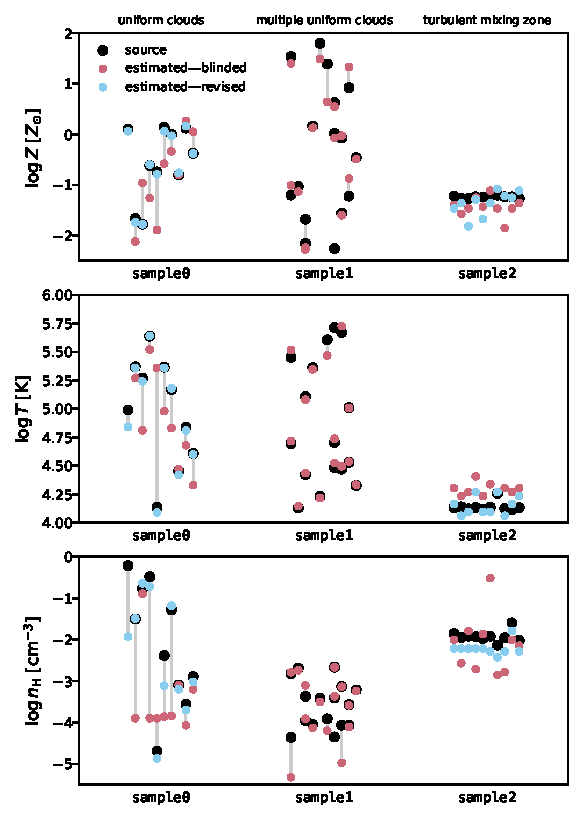
\includegraphics[width=\columnwidth]{figures/averages.pdf}
    \caption{
    The source properties (black) used to produce the synthetic absorption systems
    compared to the best estimates from parameter estimation across all three of our samples.
    Red are the parameter estimates from fully-blind modeling,
    and blue are the parameter estimates following any revision.
    The samples range from uniform clouds to a turbulent mixing zone.
    For the turbulent mixing zone the \ion{H}{I}-weighted average of the source data is shown.
    The parameter-estimation best estimates and the source data typically agree to $\lesssim$ ( 0.5 dex in $Z$, 0.3 dex in $T$, 1 dex in $n_{\rm H}$),
    excluding the blinded \texttt{sample0} estimates (\S\ref{s: results -- sample0}).
    }
    \label{f: summary--average}
\end{figure}

\begin{figure}
    \centering
    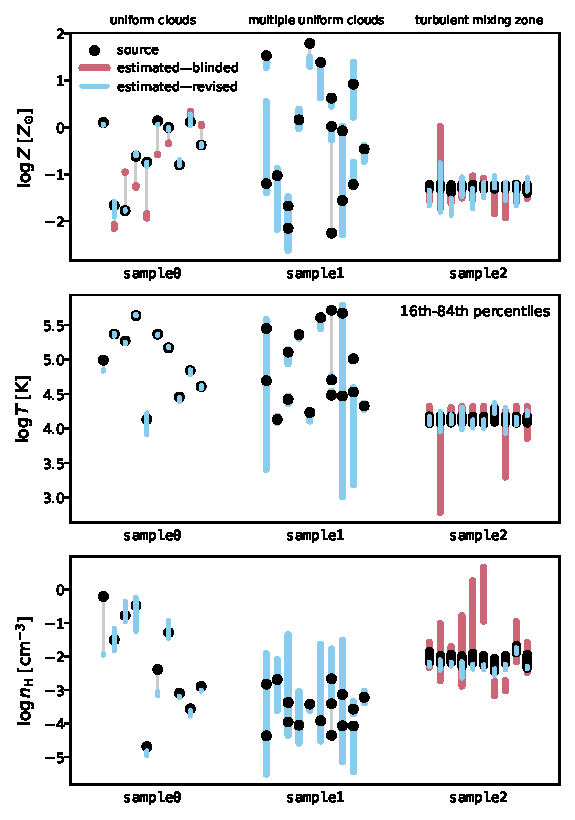
\includegraphics[width=\columnwidth]{figures/percentiles.pdf}
    \caption{
    Same as Figure~\ref{f: summary--average},
    but with lines spanning the 16th to 84th percentiles of the parameter-estimation posteriors or source data when available.
    Posteriors that overlap the source data suggest that the parameter estimation is sufficiently conservative to capture the range of possible properties for the absorbing gas.
    For \texttt{sample1} and \texttt{sample2} the posteriors typically overlap with the source data,
    with the exception of the \texttt{sample2}-revised $n_{\rm H}$ posteriors.
    For \texttt{sample0} the parameter estimation methodology had to be adapted to work with a set of provided column densities instead of full spectra,
    limiting the extent and interpretation of the provided errors.
    }
    \label{f: summary--widths}
\end{figure}

% Summary of averages
We discuss the per-sample results in the following subsections,
while Figures~\ref{f: summary--average} and~\ref{f: summary--widths} summarize some of the key results.
The agreement between the parameter-estimation best estimates and the average source properties is summarized for all three samples in Figure~\ref{f: summary--average}.
For \texttt{sample0} and \texttt{sample1} we show one value per cloud for both the source and parameter estimations.
For \texttt{sample2} the source data is a distribution of clouds, and therefore we show the \ion{H}{I}-weighted average of the source distributions compared to the \ion{H}{I}-weighted maximum likelihood estimates from parameter estimation.
The strongest disagreements are for the blinded estimates in \texttt{sample0} and \texttt{sample2}, discussed in \S\ref{s: results -- sample0} and \S\ref{s: results -- sample2} respectively.

% Summary of widths
Figure~\ref{f: summary--widths} summarizes the extent to which the source data lies within the expected range of values from parameter estimation.
In \texttt{sample0} and \texttt{sample1} the source data are discrete values per cloud,
and correspondingly we show one posterior per cloud.
In \texttt{sample2} the black lines span the 16th to 84th percentiles of the \ion{H}{I}-weighted source distributions,
and the colored lines span the 16th to 84th percentiles of the combined \ion{H}{I}-weighted posteriors (the parameter estimation in \texttt{sample2} estimates a number of clouds, and the posteriors from each individual cloud are joined into a combined posterior).

\subsection{Column densities of uniform clouds --- \texttt{sample0}}
\label{s: results -- sample0}

\begin{figure}
    \centering
    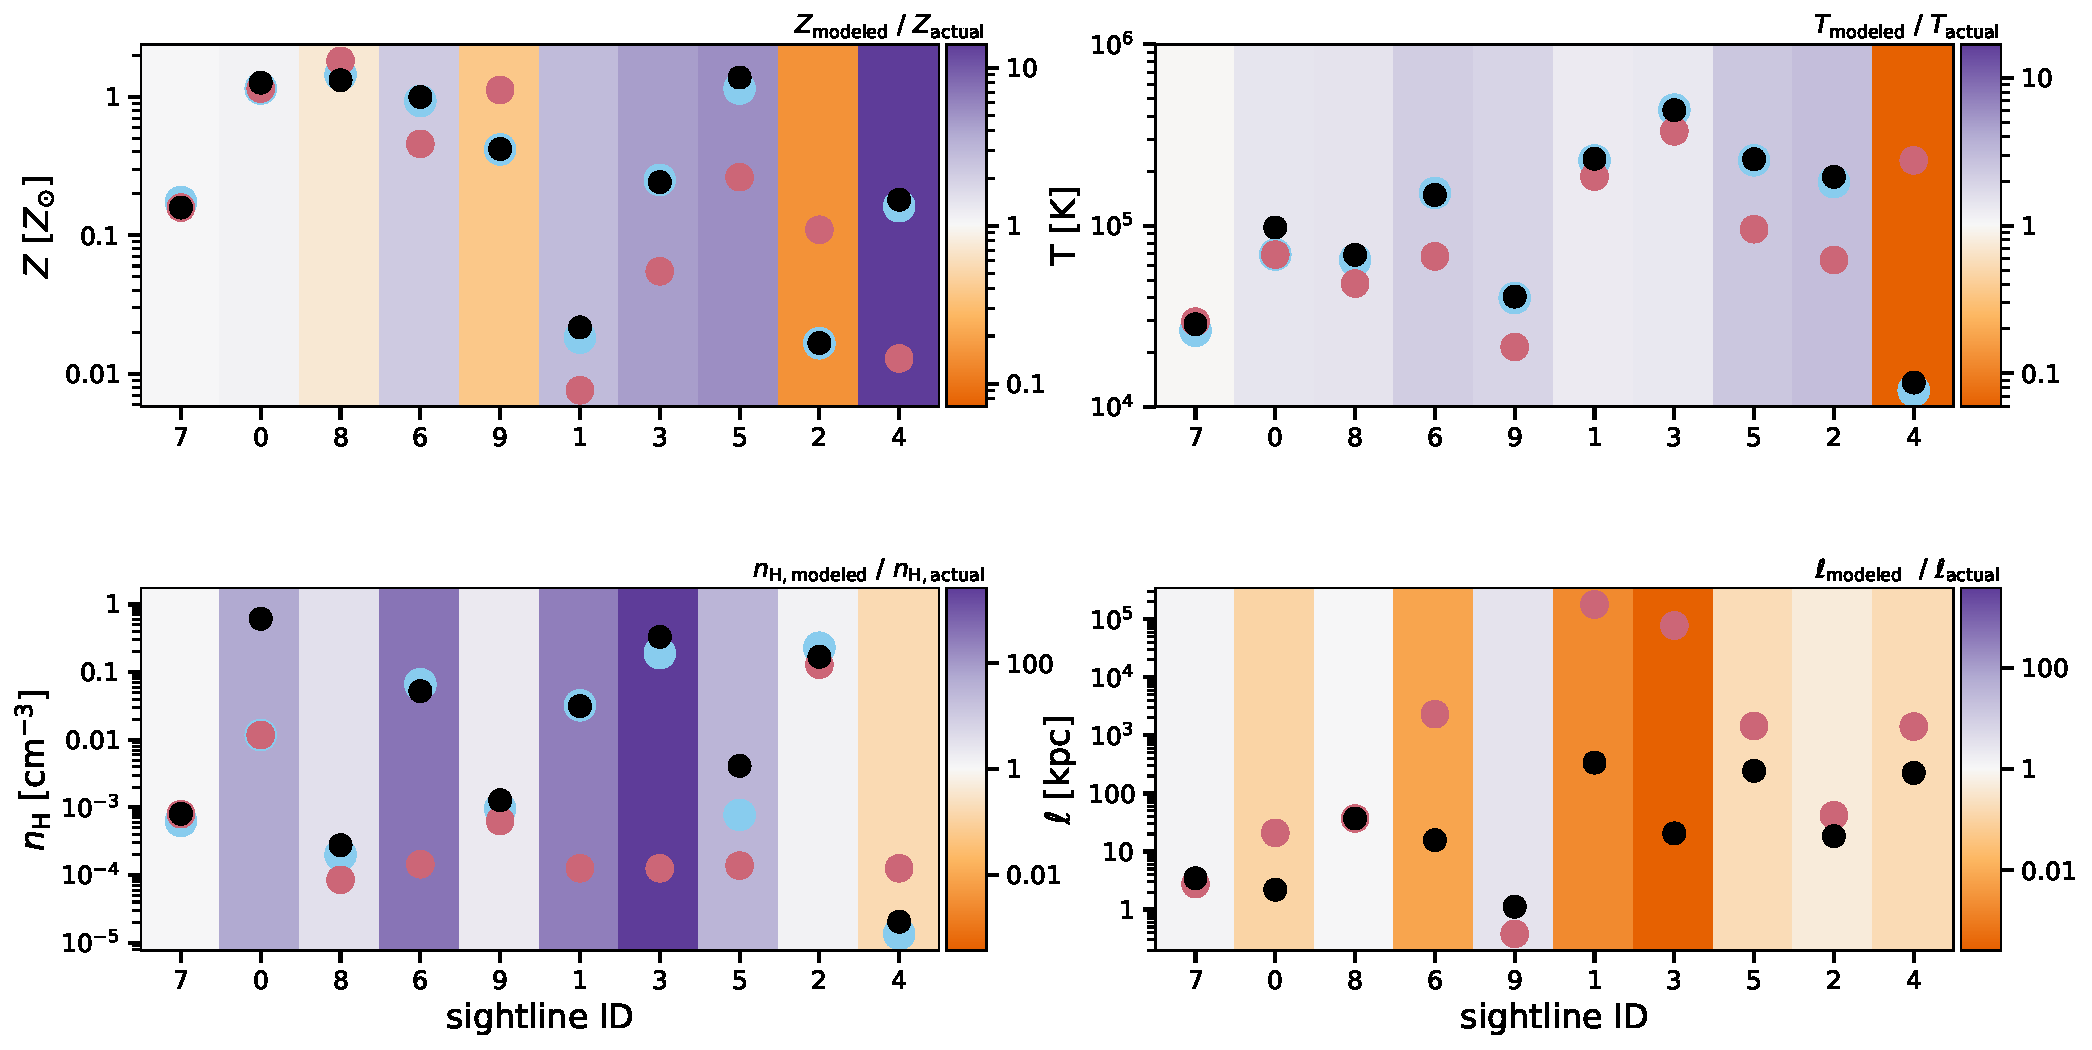
\includegraphics[width=\columnwidth]{figures/sample0/comparison.pdf}
    \caption{
    Comparison between estimated and actual properties of highly-idealized absorption systems (\texttt{sample0}).
    Sightlines are ordered from left to right according to agreement between the original modeled metallicity and the actual metallicity, and the background color indicates the level of agreement for each property.
    Black, red, and blue points show the actual, original modeled, and revised modeled values respectively for each property.
    Metallicities have agree on a better than $<0.5$ dex level for approximately half the sightlines, all of which have $Z > 0.1 Z_\odot$.
    Temperature agreement is typically $<0.5$ dex for most sightlines.
    Density and absorber length are less well-constrained, with errors up to 4 dex.
    The blind parameter estimates consistently underestimate the actual temperature and density due to the assumption of thermal equilibrium.
    }
    \label{f: idealized}
\end{figure}

\begin{figure}
    \centering
    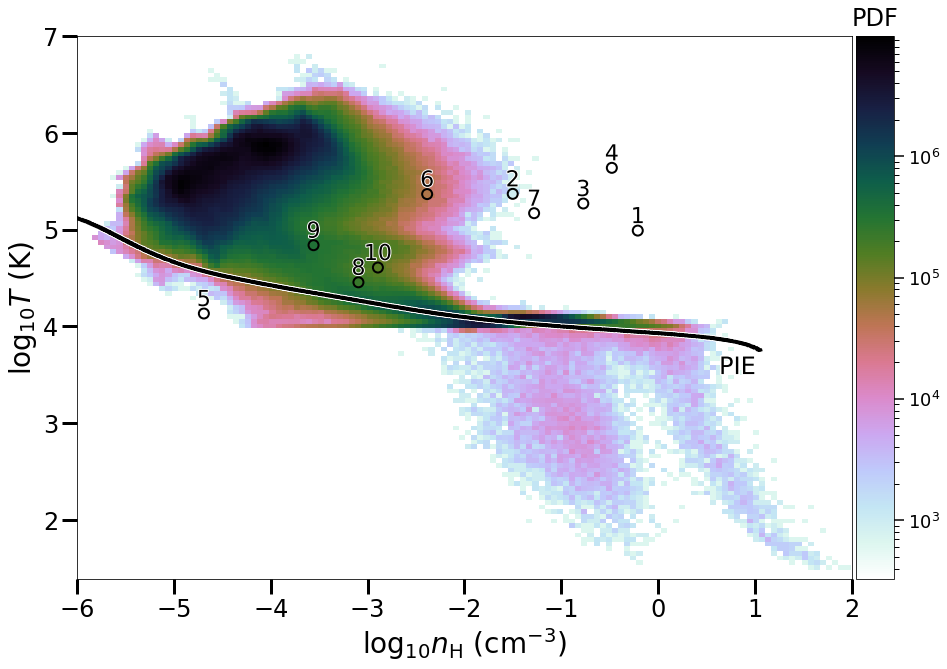
\includegraphics[width=\columnwidth]{figures/sample0/phase_space.png}
    \caption{
    Comparison between estimated and actual properties of \texttt{sample0} in the context of the phase-space distribution of CGM gas in a FIRE-2 cosmological simulation (background distribution; includes satellite ISM).
    The solid black line shows the range of temperatures and densities where gas is in thermal equilibrium via photoheating.
    \atsameer{Can you confirm this? This is the file PIEdata.csv you provided.}
    If thermal equilibrium is assumed during parameter estimation then when the assumption is inaccurate the estimated metallicity tends to be inaccurate.
    However, there is a large population of CGM gas that is in approximate thermal equilibrium.
    \todo{If this is going to be a single-column plot the font needs to be larger.}
    }
    \label{f: idealized explanation}
\end{figure}

\begin{figure*}
    \centering
    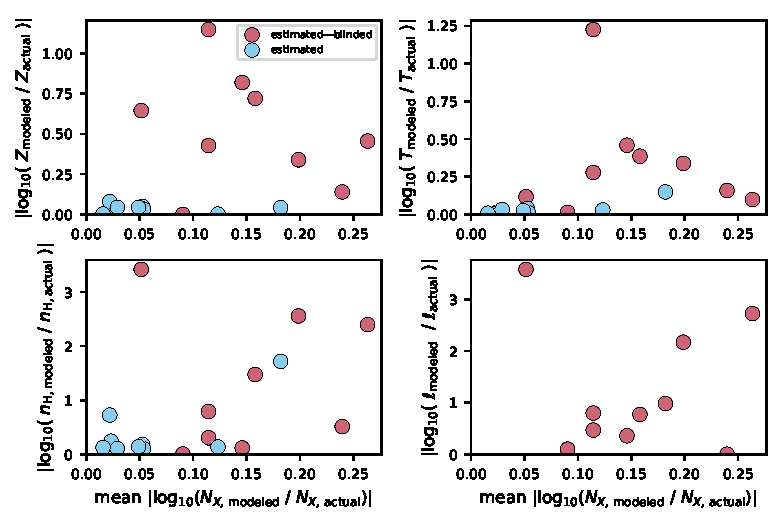
\includegraphics[width=\textwidth]{figures/sample0/error_vs_error.pdf}
    \caption{
    Error in properties of the absorbing gas vs error in column densities for \texttt{sample0}.
    The x-axis shows average log-space difference between column densities across all ions, weighted by the provided uncertainty.
    The original models fit the data decently (mean $\vert \log_{10}( N_{X,\,{\rm modeled}}$ / $N_{X,\,{\rm actual}}) \vert < 0.3$), but do not accurately recover the properties of the absorbing gas (e.g. $\vert \log_{10}( Z_{\rm modeled} / Z_{\rm actual}) \vert \gtrsim 0.4$).
    The revised models (which do not assume thermal equilibrium) recover the properties of the gas much better (e.g. $\vert \log_{10}( Z_{\rm modeled} / Z_{\rm actual}) \vert \lesssim 0.1$), and typically fit the data to mean $\vert \log_{10}( N_{X,\,{\rm modeled}}$ / $N_{X,\,{\rm actual}}) \vert \lesssim 0.05$.
    }
    \label{f: error vs error}
\end{figure*}

% A tale of priors
The discrepancies between the modeled properties and the actual properties can be understood in the context of priors.
Data generators created \texttt{sample0} by randomly sampling properties from a uniform prior for each property, independent of other properties.
However, in combination the properties were often inconsistent with common expectations of CGM gas.
This is seen in Figure~\ref{f: idealized explanation}, which compares the temperatures and densities of the source clouds to temperatures and densities typical for the CGM in a cosmological simulation.
On the other hand, the parameter-estimation team modeled \texttt{sample0} with priors constrained to regions of parameter space consistent with current knowledge of the CGM.
For example, the observers tested if the column densities were consistent with thermal equilibrium driven by photo-ionization equilibrium, in which case estimated temperature is a calculated from the estimated metallicity and density parameters, and found reasonable fits for sightlines \texttt{06} through \texttt{10}.
Observers found reasonable fits for three of the other sightlines after fixing the density to $n_{\rm H} = 10^{-3.9}$ cm$^{-3}$ and assuming collisional ionization at the model temeprature.
In this case, the temperature can be determined, but the metallicity also depends on the density,
which was not actually close to the assumed value.
In the revised modeling observers used uniform priors, e.g. no temperature-equilibrium assumptions, and found much better agreement with actual properties.
Even still, in four of the ten sightlines (\textsc{01}, \textsc{02}, \textsc{06}, \textsc{07}) the best fit parameters had total \ion{H} column densities unhandled by \textsc{cloudy}, which required observers to identify and scale solutions with the same ion densities but less total mass.

% Degenerate column densities
The above suggests reasonable agreement between modeled and actual ion column densities is possible, even when the modeled temperature, density, and metallicity are inconsistent with the actual values.
We demonstrate this in Figure~\ref{f: error vs error},
which compares the per-sightline disagreement in estimated properties to the disagreement between the estimated and provided column densities, averaged across all fit ions. 
The revised estimates are in much better agreement with the actual properties, but the revised ion column densities are adjusted by $\lesssim 0.2$ dex relative to the column densities modeled blind.
% A complicating element is that the errors data generators applied to the column densities were independent, e.g. $N_{\ion{H}{I},\,{\rm provided}} > N_{\ion{H}{I},{\rm ,actual}}$ does not mean $N_{\ion{Mg}{II},\,{\rm provided}} > N_{\ion{Mg}{II},\,{\rm actual}}$.

To summarize,
although the \texttt{sample0} models were not realistic based on the parts of parameter space occupied by simulated data, the observational modelers were initially too rigid in their assumptions.
The lesson learned is that there will be places in the real universe where heating and cooling do not balance, and the solution that observational modelers obtain may not be unique.
This is particularly true for higher ionization gas (at higher temperatures and/or lower densities).

\atcameron{Given you generated the data, do you have additional thoughts?}

\subsection{Spectra of multi-cloud systems --- \texttt{sample1}}
\label{s: results -- sample1}

\begin{figure}
    \centering
    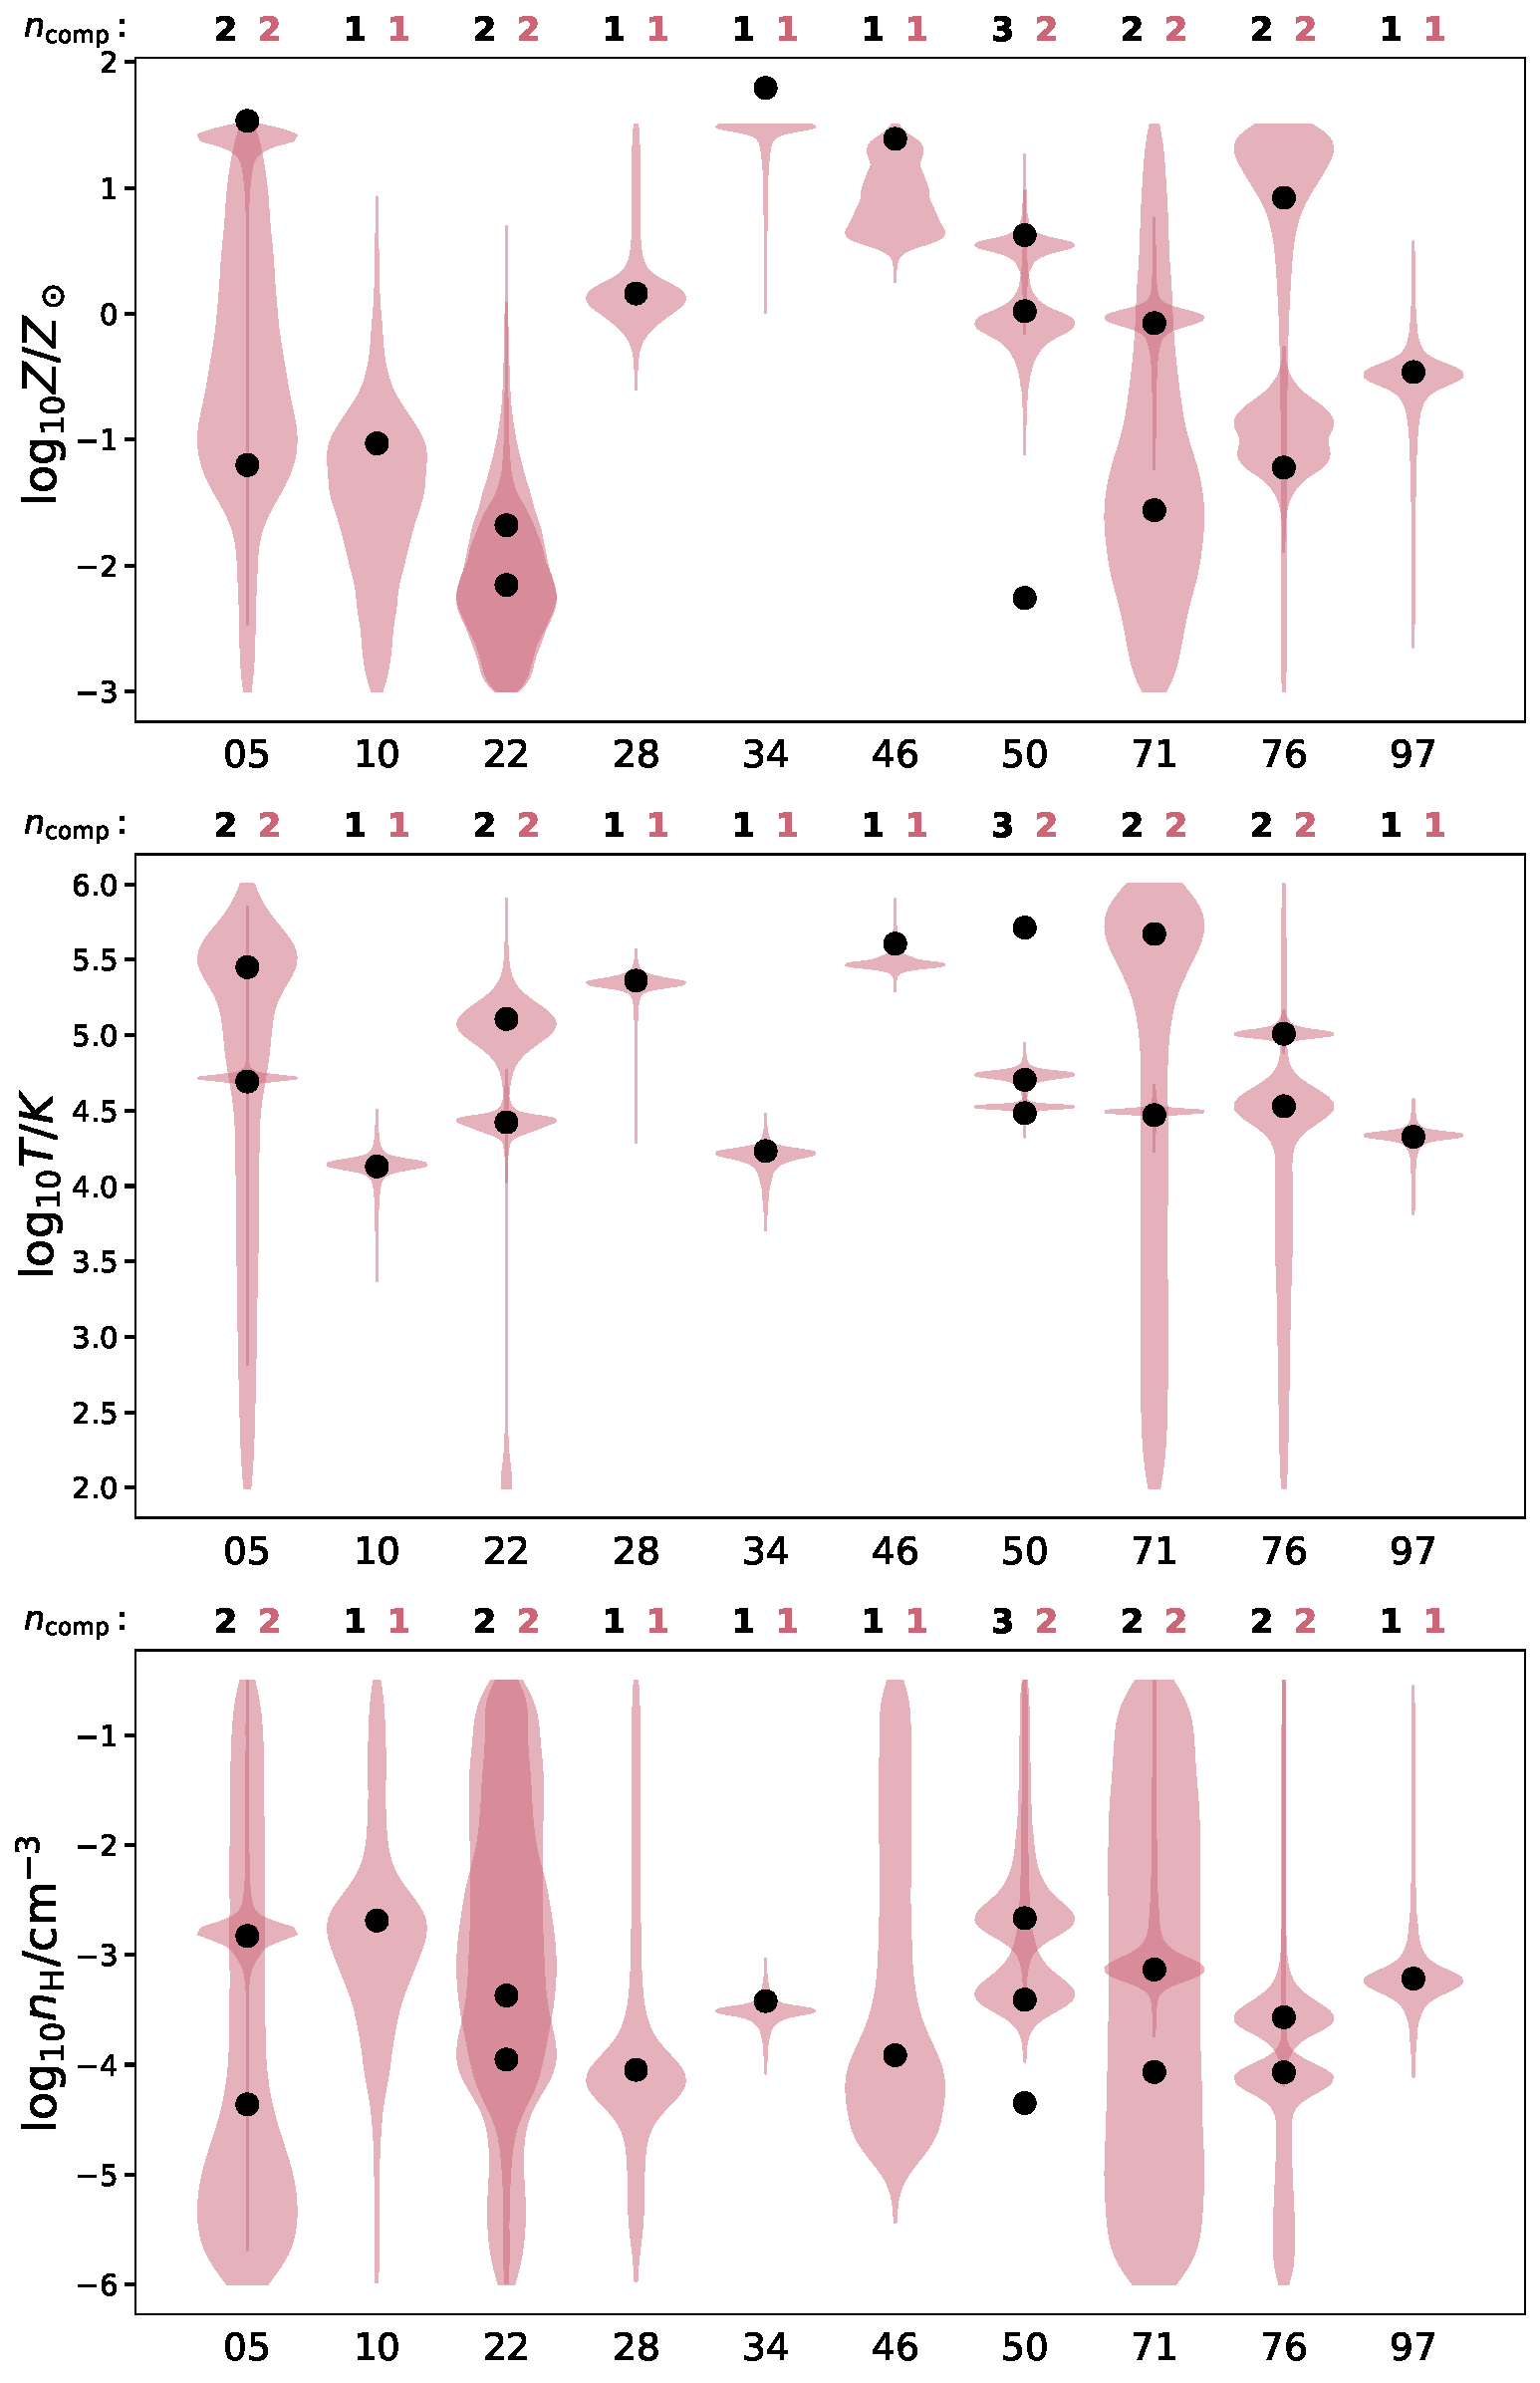
\includegraphics[width=\columnwidth]{figures/sample1/comparison.pdf}
    \caption{
    Synthetic data properties for multiple uniform clouds (\texttt{sample1}, black) compared to posteriors from parameter estimation (red).
    The numbers above each sightline indicate the number of source clouds and the estimated number of clouds.
    The maximum likelihood estimates (the peak values of the posteriors) typically align with the source parameters.
    % \todo{Do observations simultaneously get multiple properties right, or are some properties wrong while others are right?}
    \todo{Suggestion from Sameer: Instead of displaying the whole distribution as one shade, it might be better to shade region within ~1sigma as a darker shade, and the rest as a lighter shade.}
    }
    \label{f: sample1 violin}
\end{figure}

% Comparison to data
Figure~\ref{f: sample1 violin} compares the posteriors from parameter estimation to the properties of the source clouds.
In most cases the source properties reside inside the modeled distributions of possible values, i.e. the posteriors.
In other words the posteriors from modeling is, in most cases, sufficiently conservative.
As with the blind modeling for \texttt{sample0} some actual values lie outside the priors used for modeling: some actual values have $Z > 10^{1.5} Z_\odot$, while the data was modeled with a uniform prior for $Z$ spanning $log_{10} Z/Z_\odot = [-3, 1.5]$ (where $\log_{10} Z/Z_\odot = 1.5$ is the default metallicity range for Cloudy).
However, the actual values are within $< 0.5$ dex of the upper edge of the posterior, significantly less discrepant than blind modeling for \texttt{sample0}.

% Wide posteriors.
The widest posteriors in sample1 are often associated with a hotter phase tracing the OVI for a few reasons.
First, the cooling of such a gas phase resembles that of collisional time-dependent gas cooling with no external radiation, and hence is independent of density.
In two cases we also see large uncertainties in temperature, which may be due to the overlapping posteriors of two different clouds.
Second, particularly applicable for these two cases, following the lessons learnt from \texttt{sample0}, the parameter-estimation team relaxed the priors such that the lowest temperature could be $10^3$ K, while the source data has a lower bound of $10^4$.
A potential second mode is being reflected in the parameter estimates, which may not be realistic. 
Additional potential contributing factors to the wide posteriors include the absence of \ion{C}{IV} lines from in the provided spectra, 
and the stated error in the provided spectra.

% Number of components
The modeling identifies the correct number of components in 9 of 10 sightlines.
The exception is sightline 050, which has a hot, low-density, low-metallicity absorber that produces little absorption in the ions provided to the parameter-estimation team.

\subsection{Spectra of high-resolution turbulent mixing --- \texttt{sample2}}
\label{s: results -- sample2}

\begin{figure*}
    \centering
    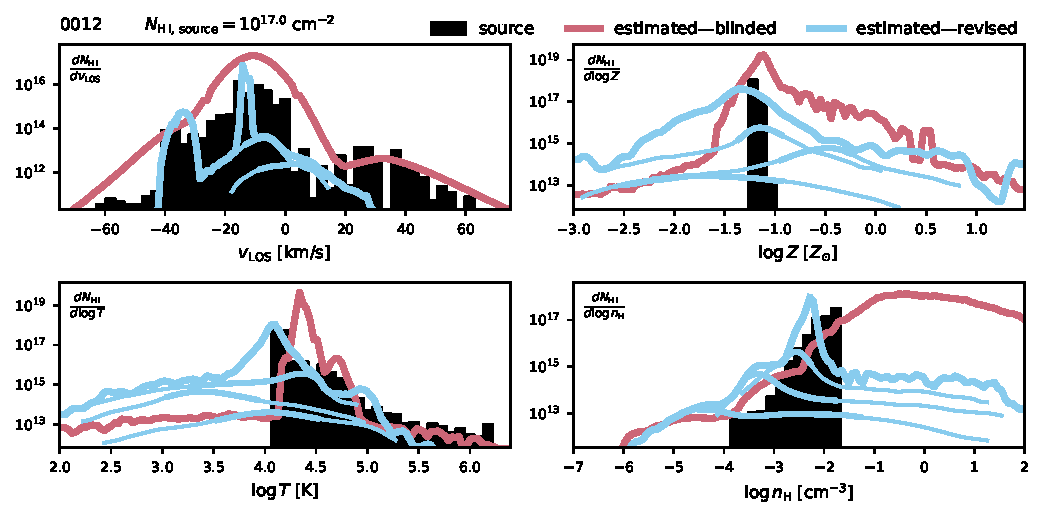
\includegraphics[width=\textwidth]{figures/sample2/high-z/sightline_0012.pdf}
    \caption{
    Estimated and source properties of gas along a sightline through a turbulent mixing zone.
    Black shows the source properties used to produce the mock spectra.
    Red and blue show the posteriors from the blinded and revised parameter estimations respectively. 
    The combined posteriors are indicated by thick lines.
    For the revised parameter estimation we also show the posteriors for the individual clouds as blue lines outlined in thick (thin) black, for the regions enclosing 68\% (99.7\%) of the posterior for a given cloud.
    }
    \label{f: sample2 12}
\end{figure*}

\begin{figure*}
    \centering
    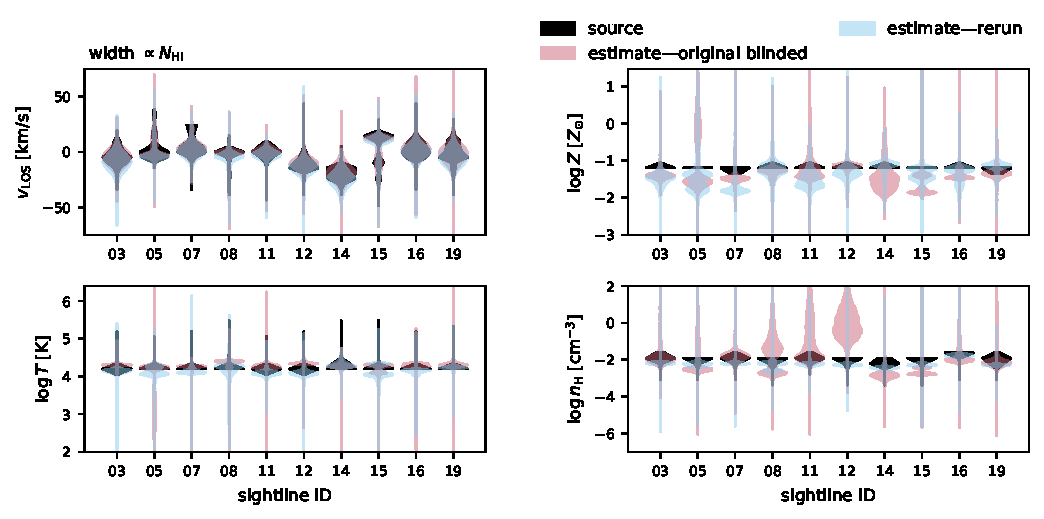
\includegraphics[width=\textwidth]{figures/sample2/violin.pdf}
    \caption{
    The distributions of $v_{\rm LOS}$, $Z$, $T$ and $n_{\rm H}$ for the synthetic source data (black) compared to the full posteriors from parameter estimation (blinded is red, blue is revised).
    The width of the violin plots scales with $N_{\ion{H}{I}}$.
    The posteriors for both the blinded and revised parameter estimations overlap with the source distributions in most cases, suggesting the parameter estimation is typically sufficiently conservative.
    Exceptions are
    both the blinded and revised posteriors of $Z$ for \texttt{07},
    the blinded posteriors of $Z$ for \texttt{14} and \texttt{15},
    most of the blinded posteriors of $T$,
    and both the blinded and revised posteriors of $n_{\rm H}$ for \texttt{12}, \texttt{14}, and \texttt{15}.
    \todo{Condense the last sentence?}
    \todo{Add legend/labels.}
    }
    \label{f: sample2 violin}
\end{figure*}


\begin{figure*}
    \centering
    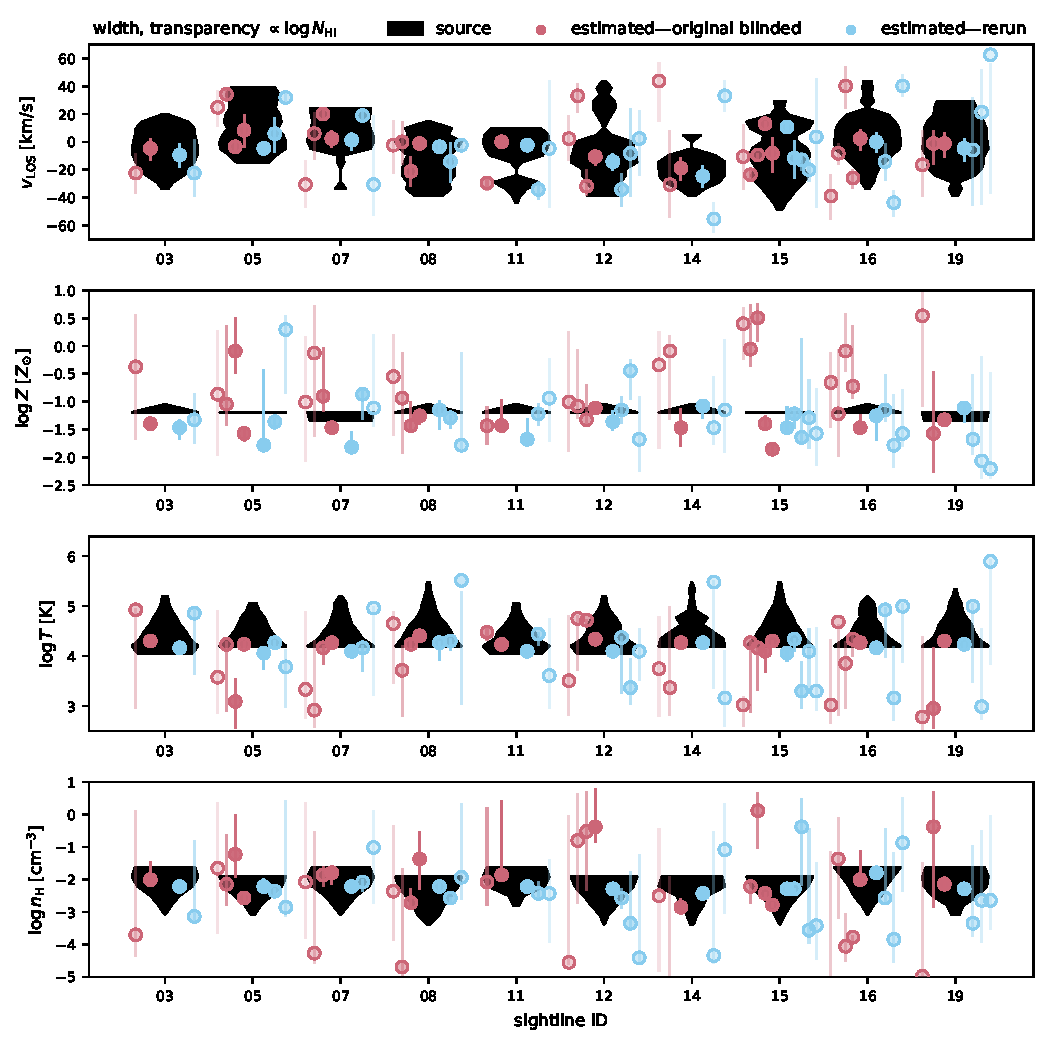
\includegraphics[width=\textwidth]{figures/sample2/violin_vs_components.pdf}
    \caption{
    The distributions of $v_{\rm LOS}$, $Z$, $T$ and $n_{\rm H}$ for the synthetic source data (black) compared to the best estimates for individual components comprising the parameter estimation.
    Each point is the maximum-likelihood estimate (MLE) of an individual component,
    and the associated bars enclose the the 16th to 84th percentiles of the posterior.
    The width of the violin plots and the opacity of the points are scaled \textit{logarithmically} with $N_{\ion{H}{I}}$,
    such that if the parameter estimation perfectly agreed with the data all visible MLE points would lie within the source data violins.
    The MLE of the strongest component typically aligns with the peak of the source distribution, but can be off by $\lesssim 1$ dex for $Z$ and $n_{\rm H}$, especially for the blinded estimates.
    The best fit for parameter estimation consistently includes lower-column-density components with properties not found in the source data.
    \todo{Make visual signifier of logscale.}
    \todo{Ensure the vlos distribution has sufficiently small bins.}
    }
    \label{f: sample2 violin vs components}
\end{figure*}

% \begin{figure*}
%     \centering
%     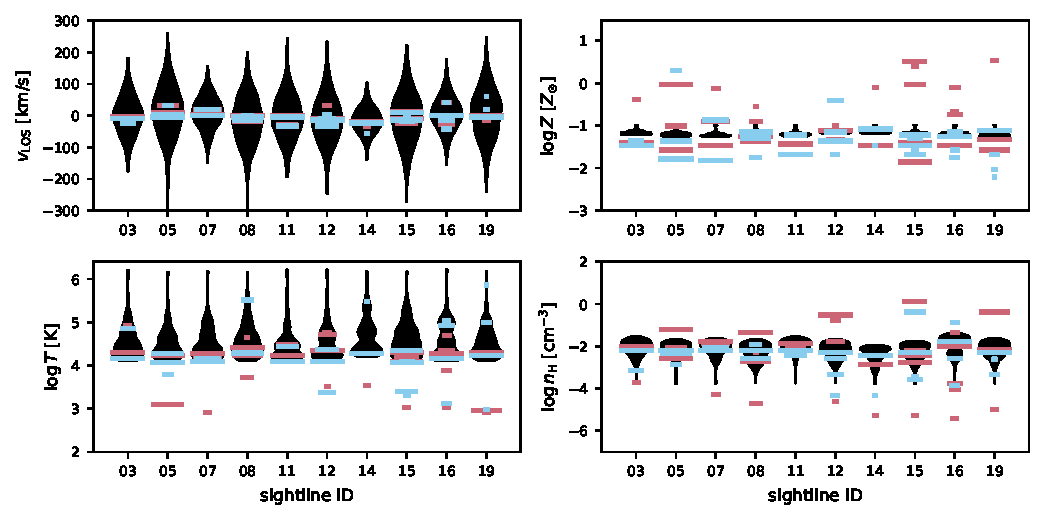
\includegraphics[width=\textwidth]{figures/sample2/violin_vs_components_alternate.pdf}
%     \caption{
%     Alternative version of the preceding figure.
%     The distributions of $v_{\rm LOS}$, $Z$, $T$ and $n_{\rm H}$ for the synthetic source data (black) compared to the best estimates for individual components comprising the parameter estimation.
%     Each horizontal line is the maximum-likelihood estimate (MLE) of an individual component.
%     The width of the violin plots and horizontal lines scales \textit{logarithmically} with $N_{\ion{H}{I}}$.
%     The MLE of the strongest component typically aligns with the peak of the source distribution, but can be off by $\lesssim 1$ dex for $Z$ and $n_{\rm H}$, especially for the blinded estimates.
%     The best fit for parameter estimation consistently includes lower-column-density components with properties not found in the source data.
%     \todo{Make visual signifier of logscale.}
%     }
%     \label{f: sample2 violin vs components alt}
% \end{figure*}

% \begin{figure*}
%     \centering
%     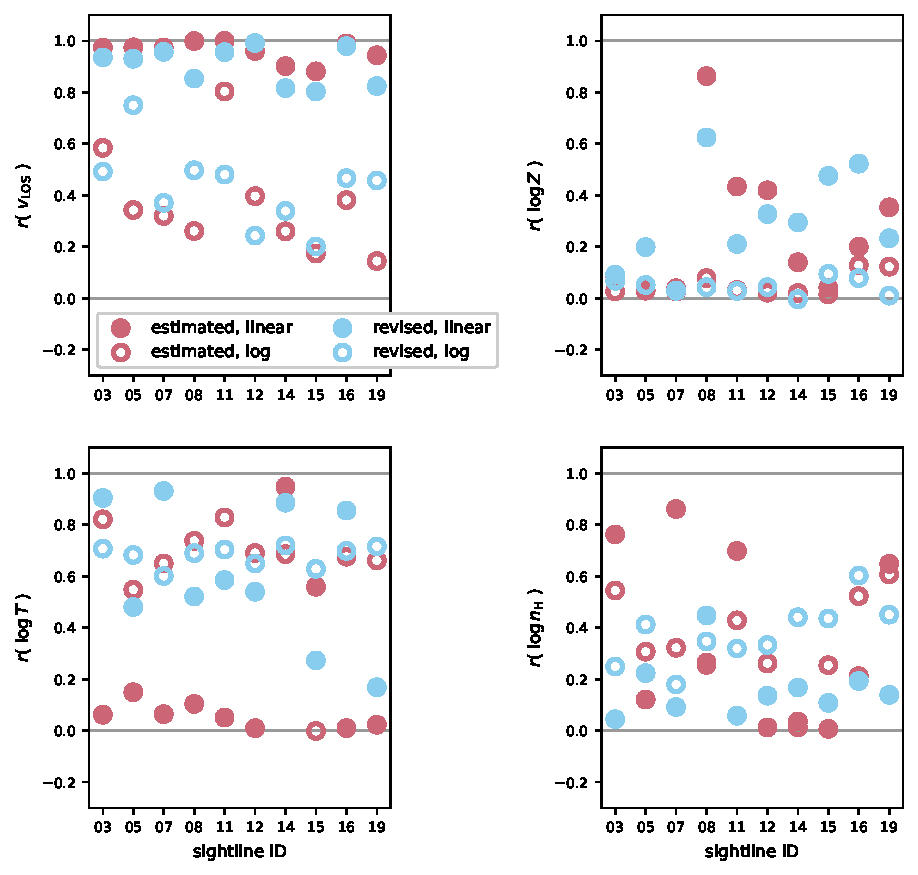
\includegraphics[width=\textwidth]{figures/sample2/correlations.pdf}
%     \label{f: sample2 correlations}
%     \caption{
%     Correlation coefficients between the likelihood distributions estimated by  parameter estimation and the actual distributions of gas properties.
%     The gas probed is found along sightlines through a high-resolution simulation of turbulent mixing zones (\texttt{sample2}).
%     The results of fully-blind modeling is shown in red.
%     The revised results are shown in red.
%     The largest change is that the revised modeling provides a much better estimate of the temperature.
%     \todo{Some of the poor disagreements are because the predicted distribution is poorly constrained, not because it outright disagrees.
%     We should find a way to show this, maybe via comparing the MLE to the peak of the distribution?
%     This might also be a quantity that's easier to interpret.
%     Basically we want two quantities: one that compares disagreement in peak values, and one that compares overall match in distributions.}
%     \todo{Clarify that linear/log refers to the y-axis.}
%     }
% \end{figure*}

% Individual example
Figure~\ref{f: sample2 12} shows parameter estimation for a single sightline, sightline 12, which is best fit by four clouds.
Both the source data and the posteriors are normalized by associated \ion{H}{I} column density.
Integrating over the source data for any property yields the total \ion{H}{I} column density.
Integrating over any property posterior for a component yields the median estimated \ion{H}{I} column for that component.
The combined posterior is the result of co-adding the normalized single-component distributions.
The maximum likelihood estimate of the combined distribution is usually dominated by the strongest component,
agrees relatively well with the peak values of the source data.
The lower-column-density components are not perfect tracers of the source distribution, but still capture some features.
For example, the four peaks (MLEs) of the individual cloud posteriors approximately span the high-$T$ and low-$n_{\rm H}$ source data.

% Strongest component
Figure~\ref{f: sample2 violin} compares the parameter-estimation posteriors to the source data property distributions.
Each violin shape is a 1D distribution like those shown in Figure~\ref{f: sample2 03}, rotated 90 degrees and scaled linearly.
The linear scale emphasizes the dominant $v_{\rm LOS}$, $Z$, $T$ and $n_{\rm H}$ for both the source and parameter estimation.
The shape of the $v_{\rm LOS}$ posteriors closely traces the actual distribution of $v_{\rm LOS}$ for both parameter estimations.
The metallicity is accurate to within $\lesssim 1$ dex,
and the temperature and density are accurate to within $\lesssim 0.5$ dex.
Due to changes in the redshift at which the synthetic data is ``viewed'', the revised estimates are in better agreement with the source data,
as discussed below.

% Component structure
Figure~\ref{f: sample2 violin vs components} reveals the extent to which parameter estimation can capture the structure of the source distributions.
Each violin is proportional to the \textit{logscale} 1D source-data distribution,
where only regions of the distribution that provide $N_{\ion{H}{I}} > 10^{13}$ cm$^{-2}$ are shown.
This value was selected because there are no parameter-estimation components with lower column densities.
To be precise at the risk of increased complexity,
for e.g. $\log Z$ we set the thickness of the violin to zero for $\frac{dN_{\ion{H}{I}}}{d\log Z} < 10^{13} {\rm cm}^{-2} / (\log Z_{\rm max} - \log Z_{\rm min} ) \approx 10^{13} {\rm cm}^{-2} / ( 1.5 - (-3) )$.
The points show the MLEs for each component the parameter-estimation fit is composed of,
with the opacity scaled logarithmically by $N_{\ion{H}{I}}$ of the component.
The components become completely invisible as $N_{\ion{H}{I}} \rightarrow 10^{13}$ cm$^{-2}$.
The presence of component MLEs with properties not found in the source data demonstrates the current limits of parameter estimation---extracting the detailed structure of the absorbing gas is not achieved.
However, as shown by the agreement in the strongest MLEs and the peaks of the source data,
parameter estimation does well in estimating the average properties of the absorbing gas.

% Blinded sample
The primary difference between the blinded and revised estimates lies in the source data,
rather than the estimation methodology.
The temperature, density, metallicity, LOS velocity, and total column for \texttt{sample2} were extracted from $z=2$ sightlines passing through a high-resolution simulation of a turbulent mixing zone.
To avoid providing any hints about the origin of the data the synthetic generators aimed to provide $z \sim 0 - 0.25$ spectra,
as was done for the preceding samples.
To this end, for the blinded \texttt{sample2} the synthetic generators took the $z=2$ absorbing-gas properties,
generated spectra using the $z=0.13$ UV ionization table,
and provided synthetic observations mimicking COS observations of gas at $z=0.13$.
The concept was to generate absorption from $z=0.13$ gas,
independent of the mechanisms responsible for setting the properties of the gas.

% Revised sample
The revised \texttt{sample2} synthetic spectra used a $z=2$ ionization table,
had a wavelength resolution of 0.05 \AA,
a line spread function with a FWHM of 7 km/s,
and included the ions \ion{H}{I}, \ion{Si}{II}, \ion{Si}{III}, \ion{Si}{IV}, \ion{C}{II}, \ion{C}{III}, \ion{C}{IV}, \ion{O}{I}, \ion{O}{VI}, \ion{N}{II}, \ion{N}{V}, \ion{Fe}{II}, \ion{Mg}{X}, and \ion{Ne}{VIII}.
The ($Z$, $n_{\rm H}$, $T$, $\NHI$) of the source data were not modified.
These changes followed discussion between the data-generation and parameter-estimation teams.
The better agreement between the revised parameter estimation and the source properties is likely related to the changes in the provided spectra.
For example, the blinded estimates of $T$ are consistently high by $\sim 0.1$ dex,
while the revised estimates agree better.

\atsameer{Commentary for this sample?}

\section{Discussion}
\label{s: discussion}

\thoughts{Additional discussion topics or expansion of existing topics.}

\subsection{What data is required for accurate modeling?}

% Column densities vs spectra
Following a survey of the potential participating observers we provided ion column densities for \texttt{sample0}, instead of providing ion spectra.
The motivation was to decrease the barrier for participation in the challenge by skipping the extraction of column densities from the spectra.
However, the observers that did participate employed a parameter-estimation pipeline built to accept spectra as input.
Therefore providing the column densities as the synthetic data both required the parameter estimation team to adapt their pipeline, and limited the information we could extract.
\atsameer{In the single uniform cloud scenario, what information is contained in the profile shapes that is not contained in the column densities? Just the $b$ values?}
\atsameer{Given that it's often not possible to extract any substructure beyond different velocity components (Figure~\ref{f: sample2 violin vs components}), does that lessen the requirements to have good profile shapes?}

% High ionization absorbers
Throughout the analysis, the properties of $T \gtrsim 10^5$ K gas are more poorly-constrained than lower-temperature gas---a consequence of the parameter-estimation team not having access to high-ionization states.
Modeling of the full phase space of CGM gas requires ions such as \ion{Ne}{VIII} and \ion{Mg}{X}.
Intermediate ionization states,  especially strong ions such as \ion{C}{IV}, play an important role in separating gas phases.
Lyman series lines also improve the ability to separate phases.
\atsameer{Here I've transferred comments from Jane, re: the utility of intermediate ions and Lyman series lines. Can you talk about how you use the lines to separate phases?}

% Data necessary to get the distributions right
For \texttt{sample2} the lines available to the parameter-estimation team provided extensive coverage of $T \sim 10^4$ K gas.
The provided data also had a high S/N, and no contamination from gas separated in physical space but overlapping in velocity space.
To that end, the data may trace a best-case scenario for detailed modeling of cloud properties.
This suggests that it may be difficult to distinguish absorption from many small clouds vs absorption from one large one.
However, parameter estimation may be more successful at this task if the many small clouds are more widely distributed in velocity space than they are in the \texttt{sample2} TMZ.
\atsameer{Is there any data you can think of where you may be able to constrain the substructure better than in Figure~\ref{f: sample2 violin vs components}?}

\todo{What data is necessary in order to get the average properties right?}

\subsection{Implications for existing results}

% For analyses that infer a physical picture from individual sightlines
Some works argue that it is possible to extract detailed information about the origin of absorbing gas, often with the aid of additional observations of the galaxy associated with the absorption system.
For example, \cite{Peroux2013} argue that one of their identified absorption systems is dominated by gas originating in and outflow, and \cite{Peroux2017} suggest that a separate absorption system has little contribution from outflows.
Making statements regarding the origin or fate of absorbing gas requires being able to identify and separate multiple clouds along a given line of sight.
Our results indicate that clouds with distinct, uniform properties can indeed be distinguished from one another successfully (Figure~\ref{f: sample1 violin}).
On the other hand, \texttt{sample2} is spectra of a filament falling in from the IGM and passing through a metal-enriched halo.
Individual clouds cannot be easily identified in the provided spectra,
but the average properties of the filament can be identified clearly,
and these properties may allow observers to constrain the \ion{H}{I}-weighted origin of absorbing gas if constraining origin via e.g. metallicity.

% For analyses that infer total masses or mass profiles
Some analyses aim to constrain total masses or mass profiles~\citep[e.g.][]{Zahedy2019a}~\todo{Lots of work on this, add a few more citations}.
Such analyses typically rely on the average properties of the gas and the total columns,
and therefore should not be especially sensitive to errors in parameter estimation.

\subsection{Modeling choices}

\subsubsection{Discrete components versus a distributions of cloud properties}

The most realistic among our samples, \texttt{sample2}, consists not of discrete clouds, but of a distribution of clouds.
Therefore any fully-successful model of the absorption system must also be of a distribution of clouds.
Such models exist~\citep[e.g.][]{stern2016Universal}, but are not commonly employed in parameter estimation.
However, because it is difficult to extract anything other than the ion-weighted averages of absorbing gas (as stated above) parameter estimation using a more-sophisticated model than individual clouds may not provide a clear improvement.

% % Interpreting posteriors of single clouds as distributions.
% Absorbers in reality are likely composed of infinitely many clouds with a distribution of properties.
% One method of estimating this distribution may be the same method, or very similar, as used to estimate the PDF for a finite number of uniform clouds.
% The argument is as follows.
% When interpreting multiple components in an absorption system the classic interpretation is discrete clouds with uniform ($Z$, $n_{\rm H}$, $T$, $\NHI$), and uncertainty reflecting data noise.
% However, we argue we can estimate $\frac{d\NHI}{dT}$ ( or $\frac{d\NHI}{dv_{\rm LOS}}$, etc.) using posteriors produced during  parameter estimation.
% For simplicity and generality of discussion during the following we will be referring to $\frac{dM}{dx}$, where $M$ is an extrinsic mass quantity (e.g. $\NHI$) and $x$ is an intrinsic property (e.g. temperature).
% Assume the total $\frac{dM}{dx}$ is well described by $q$ different distributions, i.e. $\frac{dM}{dx} = \sum_{i=1}^{q} \frac{dM_i}{dx}$.
% If we had a way to estimate each individual $\frac{dM_i}{dx}$ we could therefore estimate the total $\frac{dM}{dx}$.
% We note that $\frac{dM_i}{dx}$ is equivalently $\frac{dM_i}{dx} = M_i \frac{da}{dx}$, where $M_i$ is the total mass of component $i$ and $\frac{da}{dx}$ is defined as the fraction of mass with a given x, s.t. $\int dx \frac{da}{dx} = 1$.
% Note that while $\frac{da}{dx}$ has similar properties as the posterior $f(x)$, we have not yet argued that $f(x)$ may be a good representation of it.
% To estimate $\frac{da}{dx}$ I would argue we would want to use some method that estimates fraction of $M_i$ at a given $x$ based on
% (a) the actual fraction of $M_i$ at x, and
% (b) uncertainties in the estimation of $\frac{da}{dx}$.
% This is similar to what the method of estimating $f(x)$ does.
% Consider the limit of zero uncertainty but the absorption system having a distribution of properties instead of a single property.
% We hypothesize that the method of estimating $f(x)$ would in such a case trace produce an $f(x)$ that traces the distribution.
% We leave testing of this to future work \todo{Do we?}.
% As such, we use $f(x)$ as an estimate for $\frac{da}{dx}$. Therefore we have an estimate for $\frac{dM}{dx}$ using the estimated pdfs,
% $\frac{dM}{dx} = \sum_{i=1}^{q} M_i f(x)$, and in turn $\frac{d\NHI}{dT} = \sum_{i=1}^{q} N_{\ion{H}{I},\,i} f(T)$.
% \todo{There's at least one flaw in this argument.
% When checking the fit Sameer uses the discrete properties of multiple clouds, not multiple distributions.
% As such some of the individual clouds may "try" to balance missing data from the other clouds.
% Zach --- reread this section to understand the argument.
% }

\subsubsection{Assumptions about thermal, pressure, and ionization equilibrium}

% Thermal equilibrium
At the first step of our analysis our parameter-estimation team assumed thermal equilibrium.
This assumption resulted in inaccurate estimates of the parameters of \texttt{sample0}, though the magnitude of the errors was significantly exacerbated by providing source properties with unusual temperatures and densities.
Removing this assumption produced very good fits to the data regardless of temperature-density phase-space location.
Assuming thermal equilibrium for ease of modeling is therefore, at minimum, a risky assumption.

% Pressure equilibrium
\atsameer{Does your analysis assume anything about pressure equilibrium between different phases?}

% Ionization equilibrium
Both the parameter-estimation team and the data-generation team assumed ionization equilibrium, with contributions from both collisional- and photo-ionization.
On the data-generation side, this is a common assumption in cosmological and idealized hydrodynamical simulations, largely driven by the challenge in modeling non-equilibrium chemistry~\citep[e.g.][]{richings2014Nonequilibrium}.
However, in some cases non-equilibrium chemistry can have a significant effect on the properties of absorbing gas in the CGM, including providing one explanation for the observed bimodality in \ion{O}{VI} around low-redshift galaxies~\citep{oppenheimer2016Bimodality}.
\atsameer{Anything you want to say regarding ionization equilibrium in the parameter estimation community?}

\subsubsection{Absorption modeling ``by hand''}

There are a number of works that use a less-algorithmic, more people-driven approach to model sightlines~\citep[e.g.][]{misawa2008Supersolar, Lacki2010, rosenwasser2018Understanding, norris2021Discovery}.
The methods employed by the parameter-estimation team are based on these earlier models but with significant improvements:
\begin{enumerate*}
    \item They are automated, leading to a $\sim 10-100 \times$ decrease in time to model a system.
    \item They provide full posteriors for parameters, not just an estimate of the most-likely value a range of viable values.
    \item Temperature can be varied independently.
    \item All transitions are considered, weighted by noise level.
\end{enumerate*}
\atsameer{The above is modified text from a comment from Jane. A few questions:
Regarding the last point, Jane mentioned eliminating regions with blends. Can you elaborate?}

\subsection{Comparison to similar analyses}

% Interpreting multi-component spectra
Absorbing gas with the same LOS velocity is not necessarily co-spatial, but instead a single absorption component can correspond to multiple clouds of gas that are physically separated.
In an analysis of mock absorption spectra from cosmological simulations, \cite{Marra2022} show that only $\sim 30-50\%$ of absorption components are composed of a single, contiguous cloud, and $\sim 50\%$ of multiple clouds contributing to a single component are separated by $\gtrsim 3-12$ kpc depending on the ion.
Further, \cite{Marra2022} find that the amount of mass in common between velocity-aligned absorption from different ions varies widely, with $\sim 1/3$ of \ion{Si}{II} and \ion{C}{IV} absorbers sharing $>50\%$ of their mass.
Note that multiple well-separated clouds giving rise to absorption at the same LOS velocity is a physically-distinct scenario than a mist of clouds or a turbulent mixing zone, and corresponds more closely to \texttt{sample1} than \texttt{sample2}.

% Mock CGM analyses of robustness of modeling.
Regarding estimates of the bulk properties of gas along a LOS,
\cite{Liang2018} determined that a Bayesian method of modeling absorption lines was able to derive LOS \ion{H}{I} mass-weighted average properties.
\cite{marra2021.cosmo.sims.test.observational.modeling} confirmed this finding using a blind study of spectra from cosmological simulations of a $z=1$ Milky Way-type galaxy and a $z=0$ dwarf galaxy.
\cite{Acharya2021} test the robustness of density and metallicity to changes in the UV background, and find that these quantities are uncertain by factors of $\approx 4-6.3$ and $\approx 1.6-3.2$ respectively.
\atsameer{In addition to other locations it shows up in the paper, do you want to mention Sameer2021 here?} 

\subsection{Other questions}

The highest resolution in the simulation is $\sim$ 47 pc.
Should there be a consideration of the size scales when modeling synthetic data?
For observational data, though, we don't have such a luxury of imposing constraints.

\subsection{Recommendations}

\subsubsection{For observational modelers}

\begin{enumerate}
    \item Avoid restricting the parameter space of derived properties, including temperature, density, and metallicity. Derived properties that are overly-restricted can be inaccurate by $\gtrsim 1$ dex (Figure~\ref{f: idealized}).
    \item When possible, models should fit the data to mean $\vert \log_{10}( N_{X,\,{\rm modeled}}$ / $N_{X,\,{\rm actual}}) \vert \lesssim 0.1$, but even then the derived properties of the absorbing gas can be inaccurate to $\gtrsim 0.5$ dex ( Figure~\ref{f: error vs err}).
    \item The distribution of possible values is more informative than a single best value. Even when the best estimated value and the real value disagree, the real value is typically among the likely values (Figure~\ref{f: sample1 violin}).
\end{enumerate}

\subsubsection{For synthetic-data generators}

\begin{enumerate}
    \item Avoid generating spectra that are overly pathological. While testing the limits of  parameter estimation is useful, unusual spectra are disproportionately likely to be poorly modeled (Figure~\ref{f: idealized explanation}).
    \item Provide mock spectra when available, not just column densities, which contain much less data.
\end{enumerate}

\section{Conclusions}
\label{s: conclusions}

\todo{Summarize methods here.}

We conclude the following\ldots
\begin{enumerate}
    \item \textbf{Best estimates:} Across all three samples the maximum-likelihood estimates from parameter estimation agree well with the average properties of the absorbing gas (Figure~\ref{f: summary--average}), \textit{provided} temperature and density are allowed to vary independently as part of the fitting process (\S\ref{s: results -- sample0}).
    \item \textbf{Posterior distributions:} Even when the best fits do not agree with the average source parameters, the source parameters typically lie within the 16th to 84th percentiles of the posterior distribution, suggesting errors are typically sufficiently conservative (Figure~\ref{f: summary--widths}).
    \item \textbf{Agreement with observable absorption vs source properties:} Average agreement of $\lesssim 0.2$ dex in ion column densities can lead to errors of $\gtrsim (0.5, 0.3, 1.5, 1)$ dex in ($Z$, $T$, $n_{\rm H}$, and $\ell$) respectively (Figure~\ref{f: error vs error}). Fits that agree to $\lesssim 0.1$ dex in ion column densities typically lead to fitting source properties to within $\lesssim 0.2$ dex. \todo{Revise this to emphasize that it's for sample0, and that sample0 is limited to only column densities.}
    \item \textbf{Fit components:} Component-by-component modeling works well for a few discrete clouds (Figure~\ref{f: sample1 violin}), but does not capture the properties of a distribution of clouds (Figure~\ref{f: sample2 violin vs components}). \todo{What clouds are recovered well, and which aren't?}
    \todo{Emphasize that velocity structure can be recovered.}
    \item \thoughts{Additional key conclusions?}
\end{enumerate}

% Future work
\S\ref{s: results -- sample0} shows that reasonable agreement in ion column densities does not necessarily signal that the modeled properties are consistent with the actual properties.
However, this results is found under unusual circumstances---the parameter-estimation team was only provided with ion column densities rather than spectra, and the source data lay in a region of parameter space not typically occupied by CGM gas.
Future work might compare fit in observable parameters to fit in derived parameters for full synthetic spectra,
\todo{such as those made available following this work}.

\section*{Acknowledgements}

This work exists thanks to the Halo21 KITP virtual conference, organized by Cameron Hummels, Ben Oppenheimer, Mark Voit, and Jess Werk.
This research was supported in part by the National Science Foundation under Grant No. NSF PHY-1748958.

%%%%%%%%%%%%%%%%%%%%%%%%%%%%%%%%%%%%%%%%%%%%%%%%%%
\section*{Data Availability}

The EAGLE simulation data \citep{EagleTeam2017} and halo catalogues \citep{McAlpine2016} are publicly available. 

The inclusion of a Data Availability Statement is a requirement for articles published in MNRAS. Data Availability Statements provide a standardised format for readers to understand the availability of data underlying the research results described in the article. The statement may refer to original data generated in the course of the study or to third-party data analysed in the article. The statement should describe and provide means of access, where possible, by linking to the data or providing the required accession numbers for the relevant databases or DOIs.

%%%%%%%%%%%%%%%%%%%% REFERENCES %%%%%%%%%%%%%%%%%%

% The best way to enter references is to use BibTeX:

\bibliographystyle{mnras}
\bibliography{references, hafen_references, wijers_references} % if your bibtex file is called example.bib

%%%%%%%%%%%%%%%%%%%%%%%%%%%%%%%%%%%%%%%%%%%%%%%%%%

%%%%%%%%%%%%%%%%% APPENDICES %%%%%%%%%%%%%%%%%%%%%

\appendix

\section{Sightline-by-sightline comparisons for \texttt{sample2}}

\begin{figure*}
    \centering
    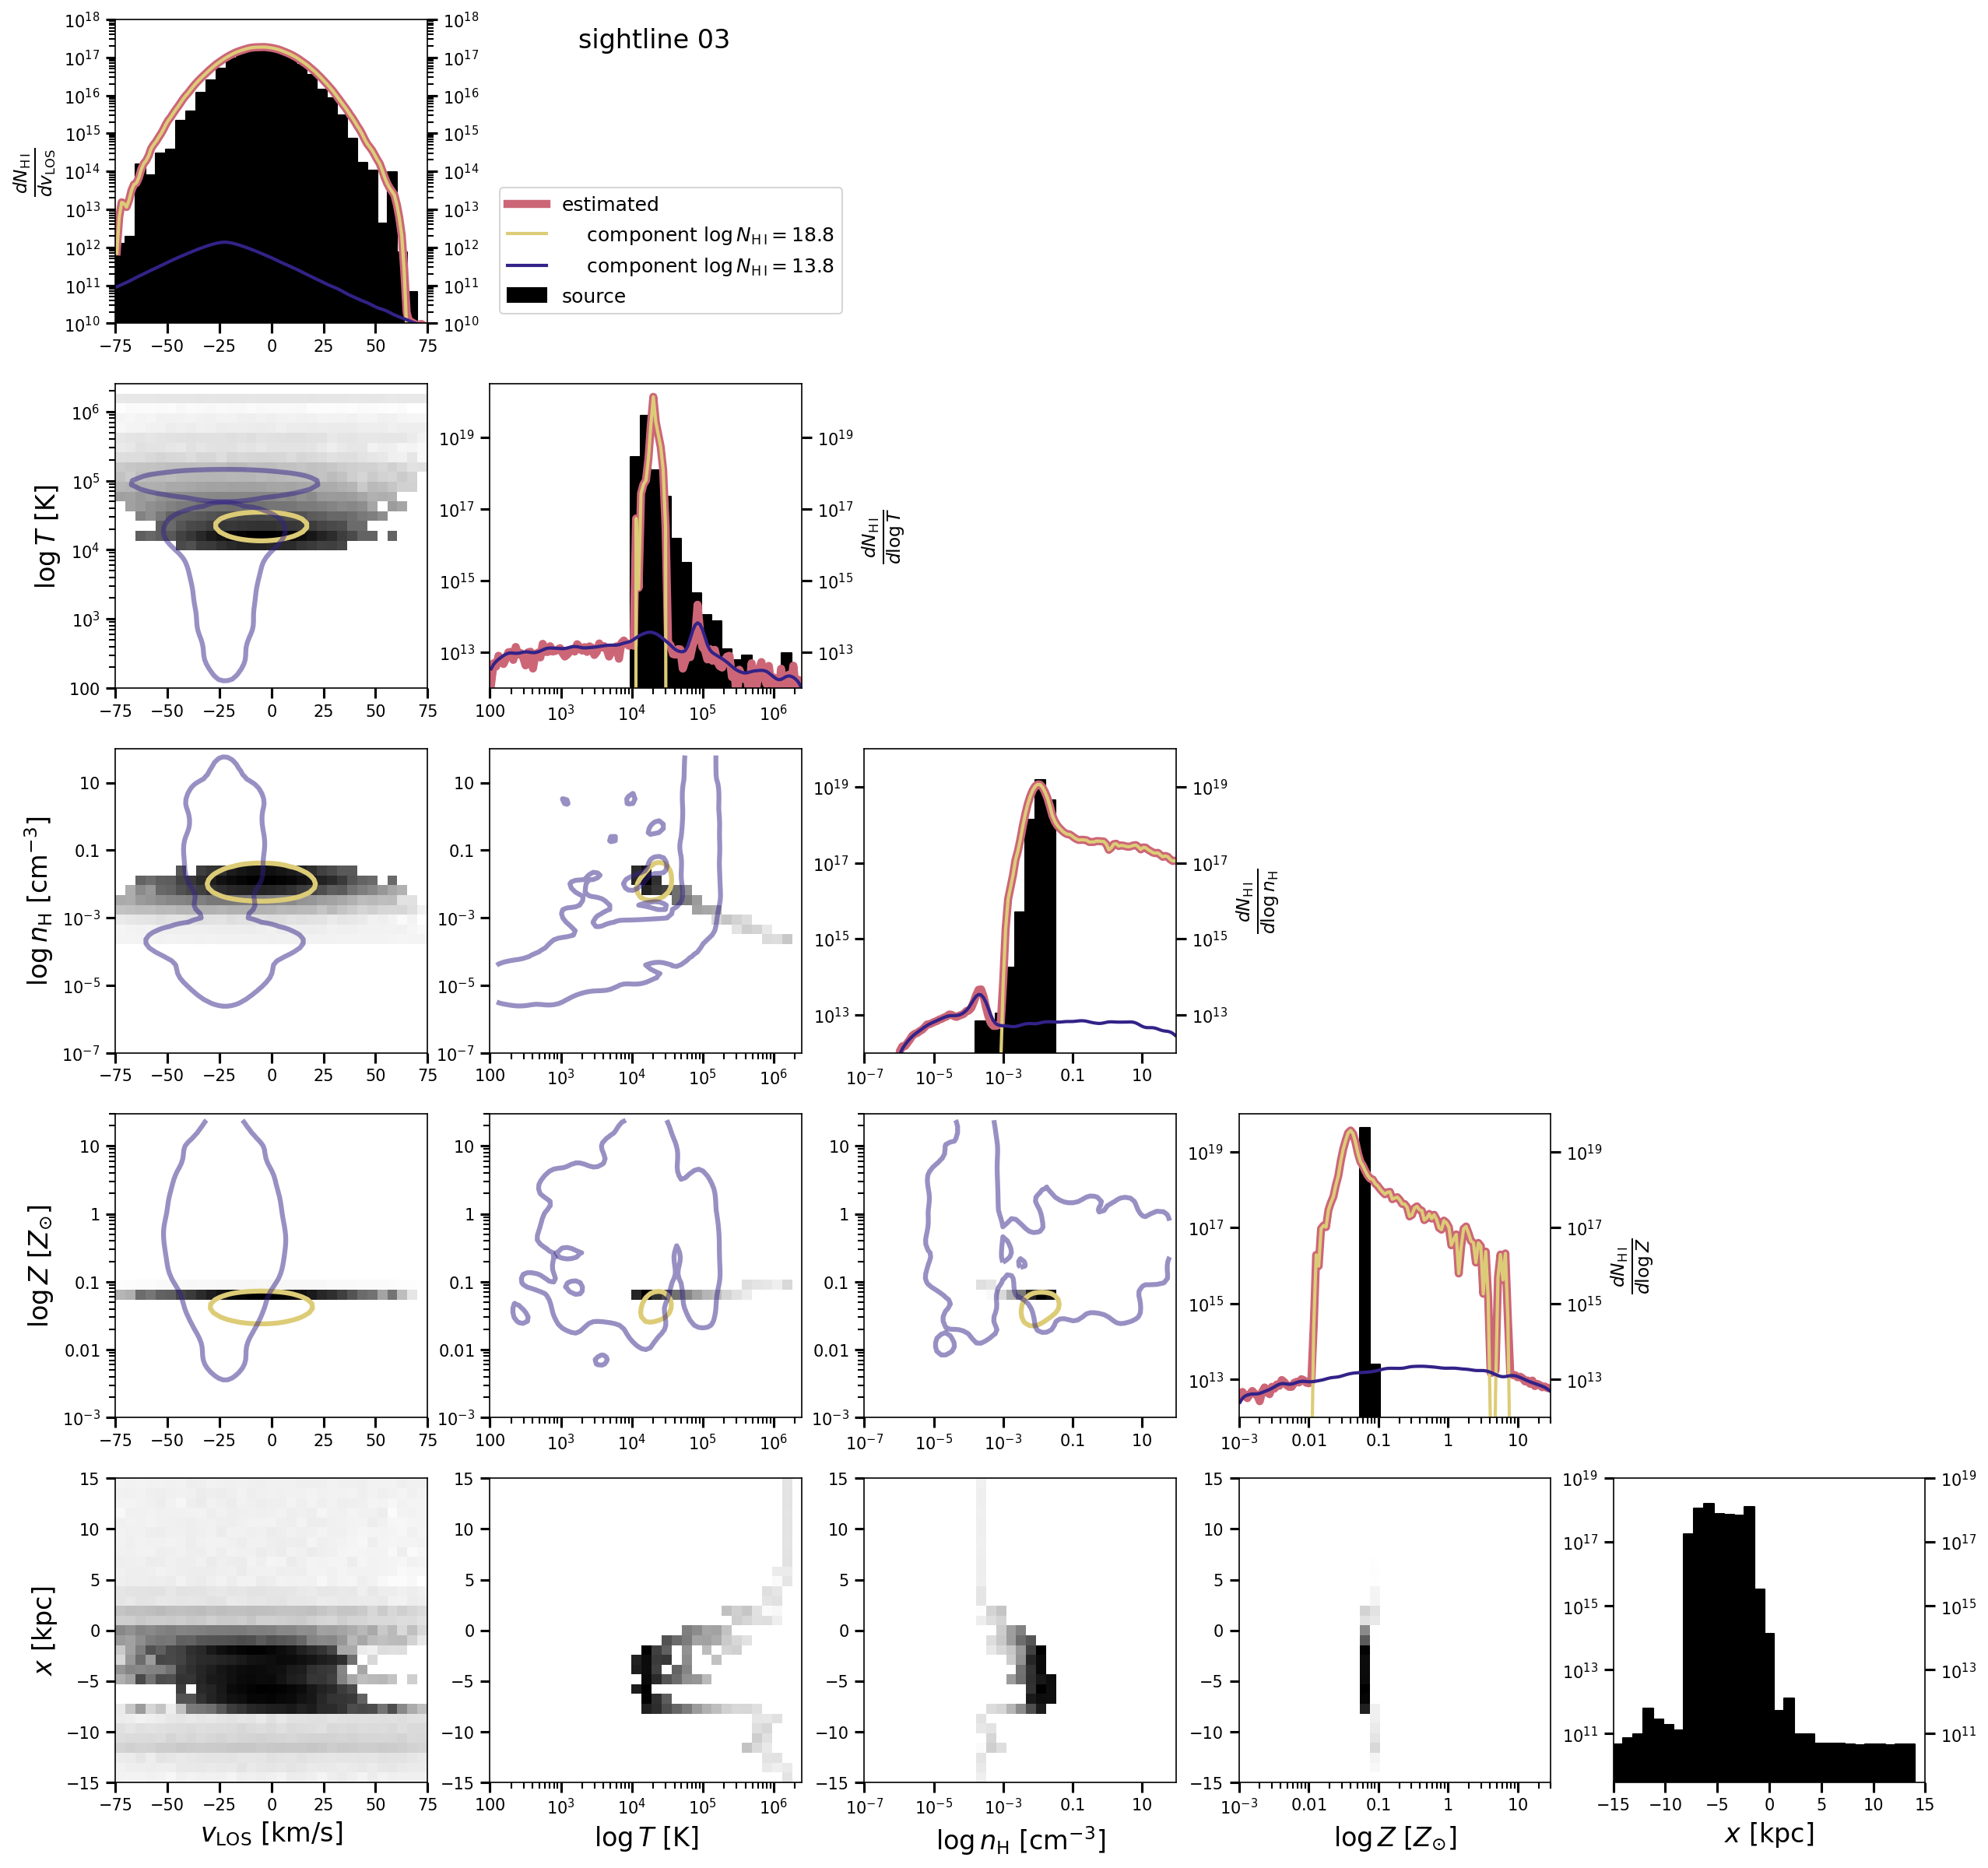
\includegraphics[height=0.45\textheight]{figures/sample2/original/sightline_0003.png}
    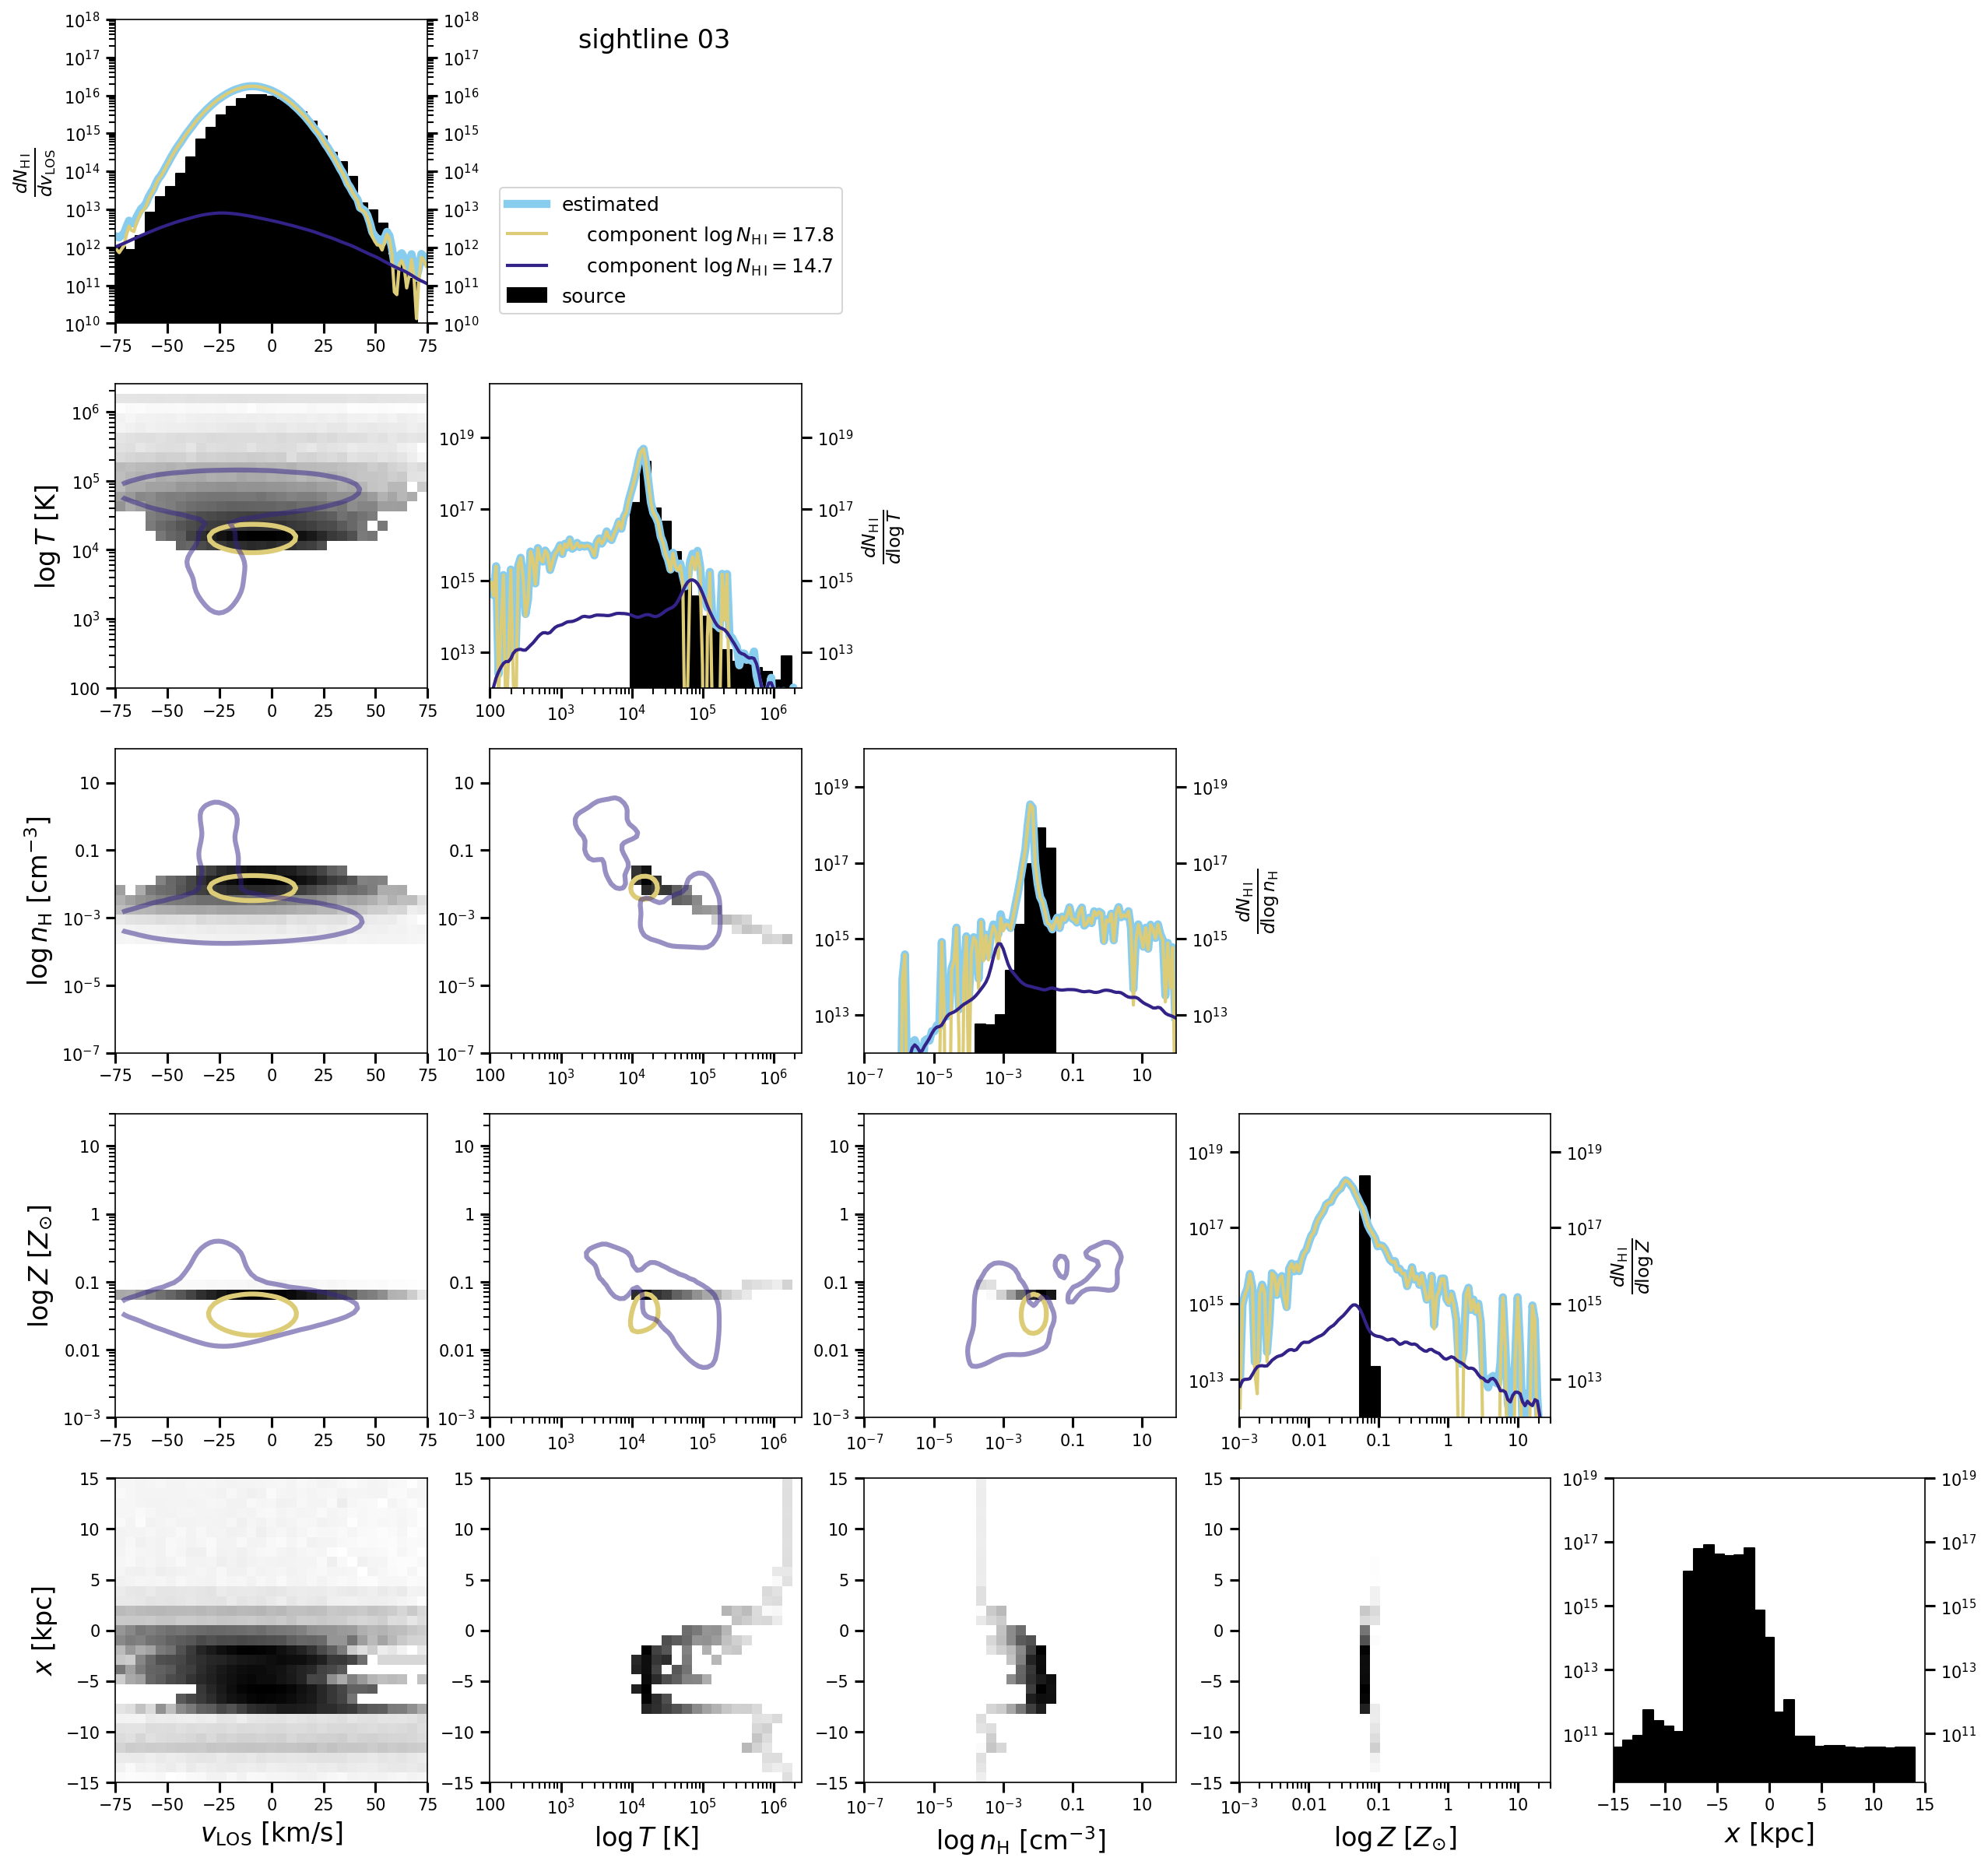
\includegraphics[height=0.45\textheight]{figures/sample2/high-z/sightline_0003.png}
    \caption{Corner plot for sightline 0003.}
    \label{f: sample2 03 corner}
\end{figure*}

\begin{figure*}
    \centering
    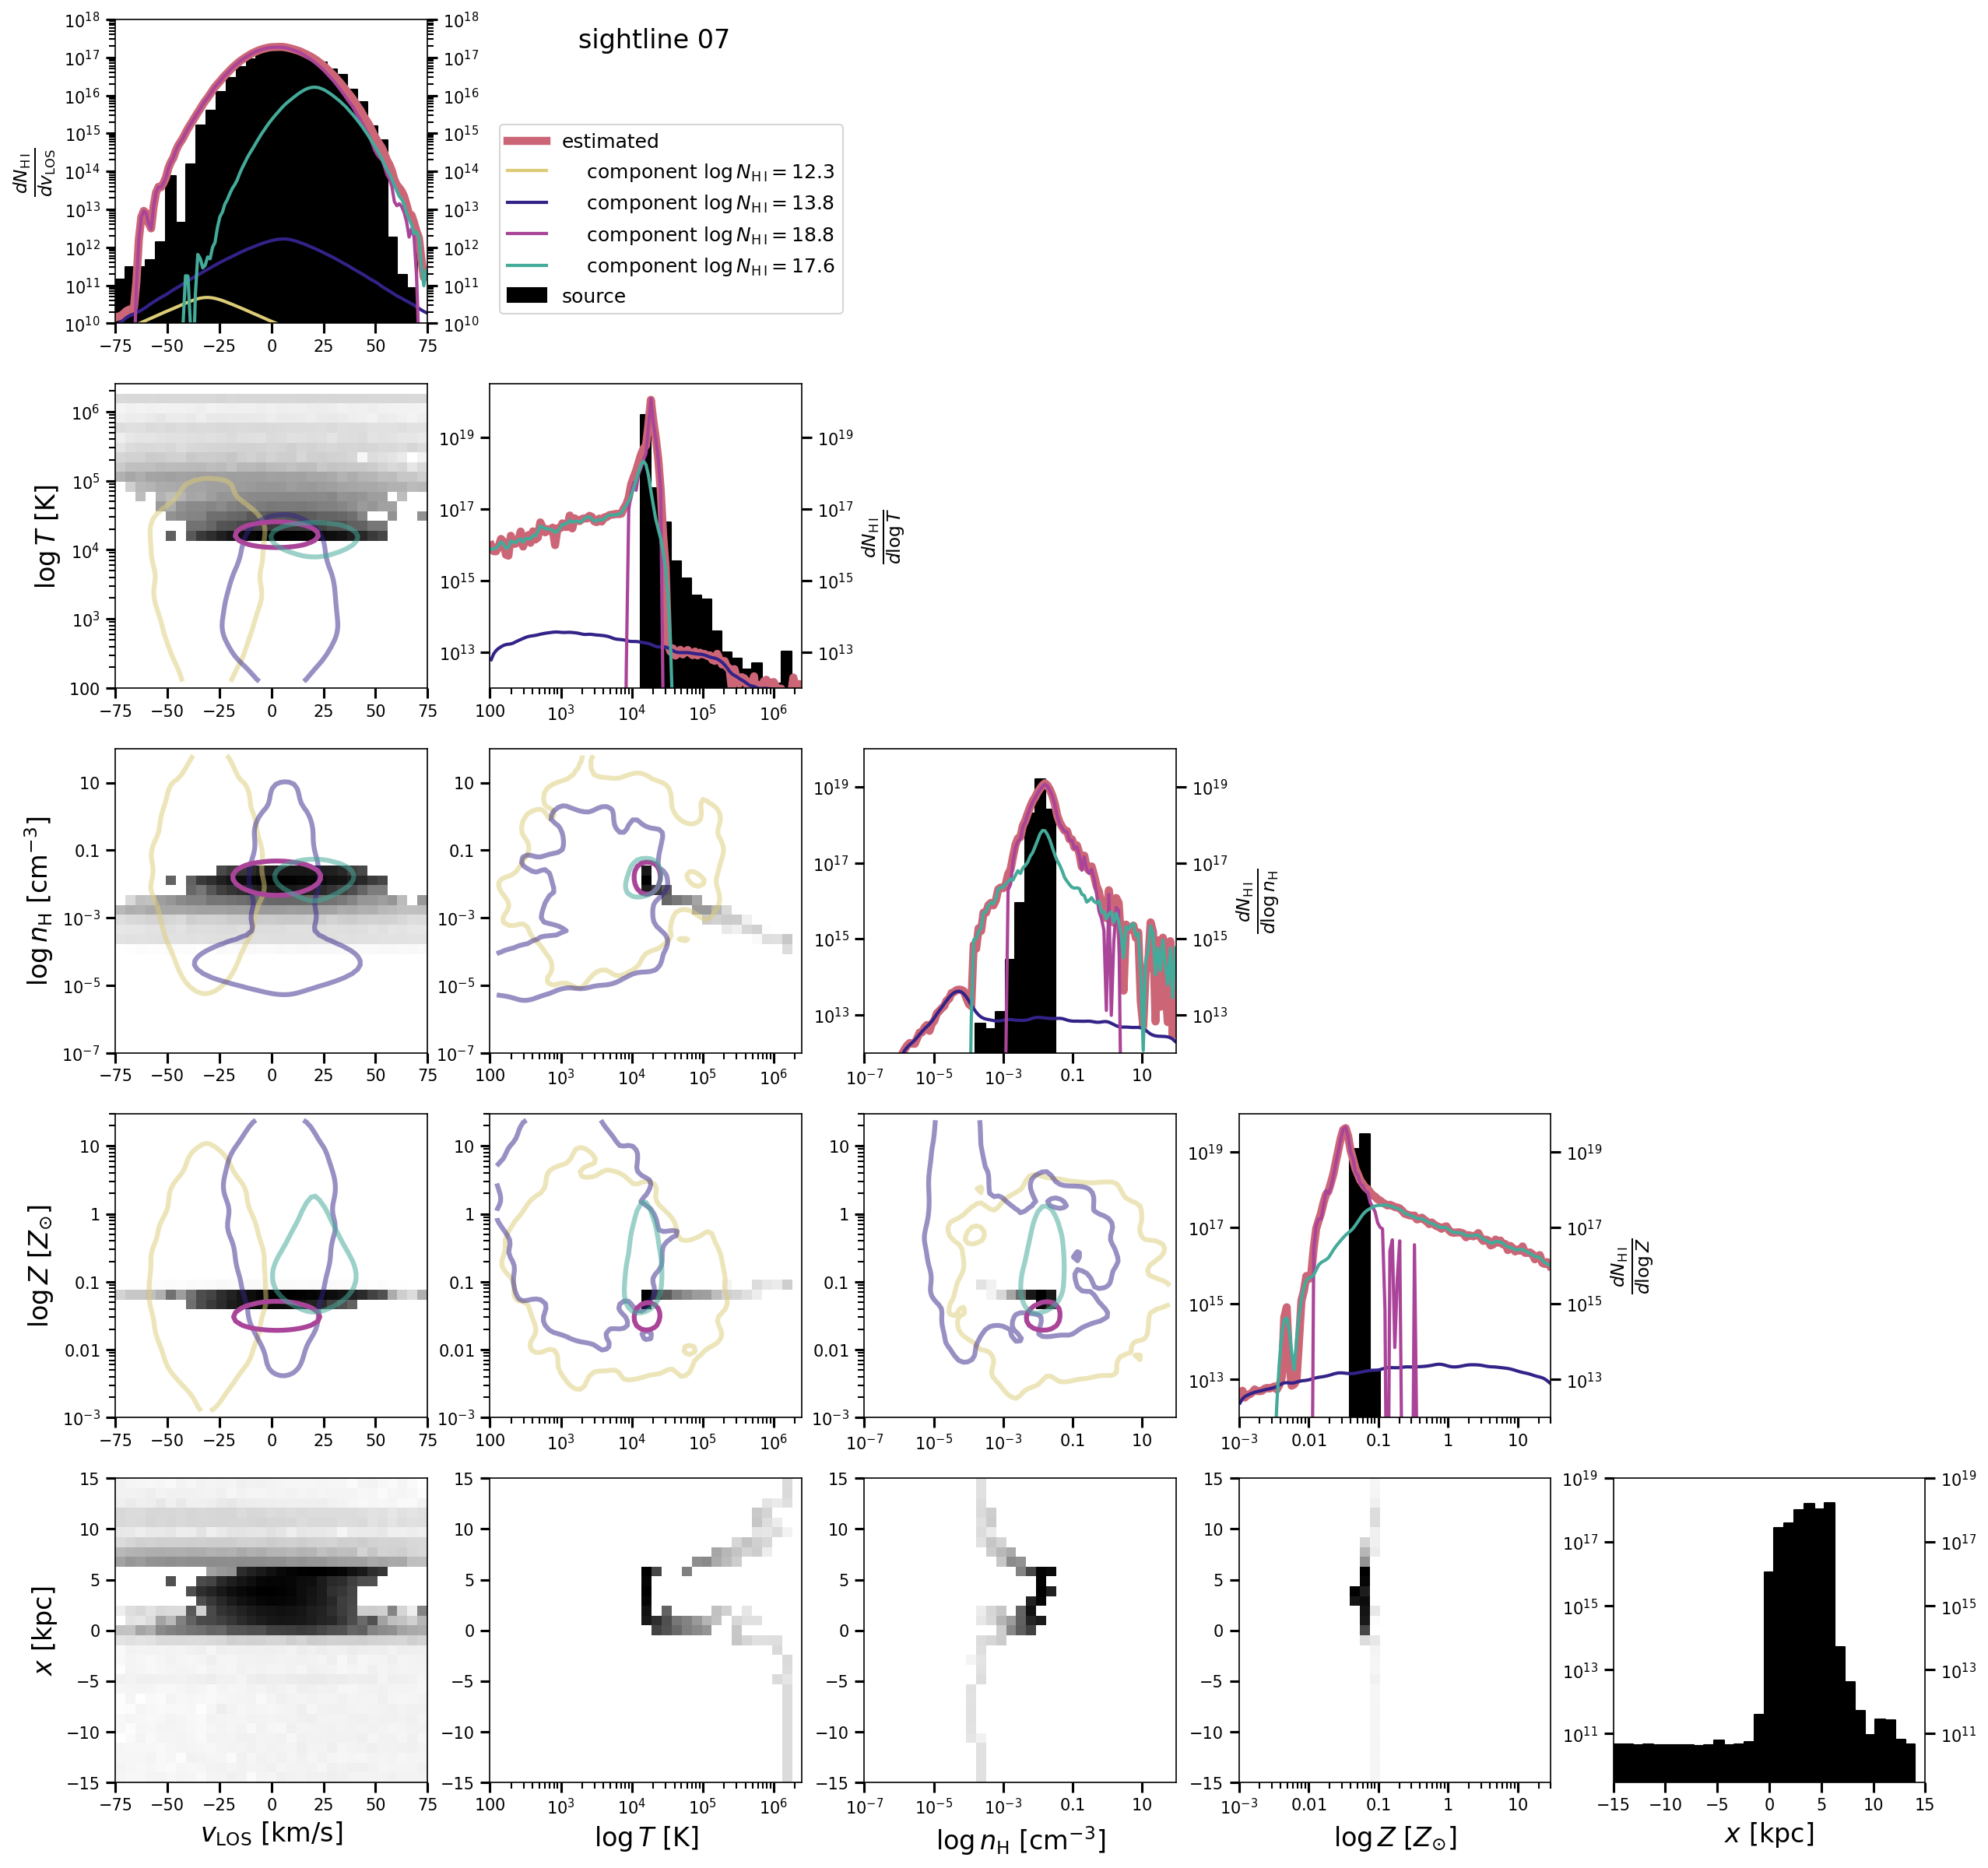
\includegraphics[height=0.45\textheight]{figures/sample2/original/sightline_0007.png}
    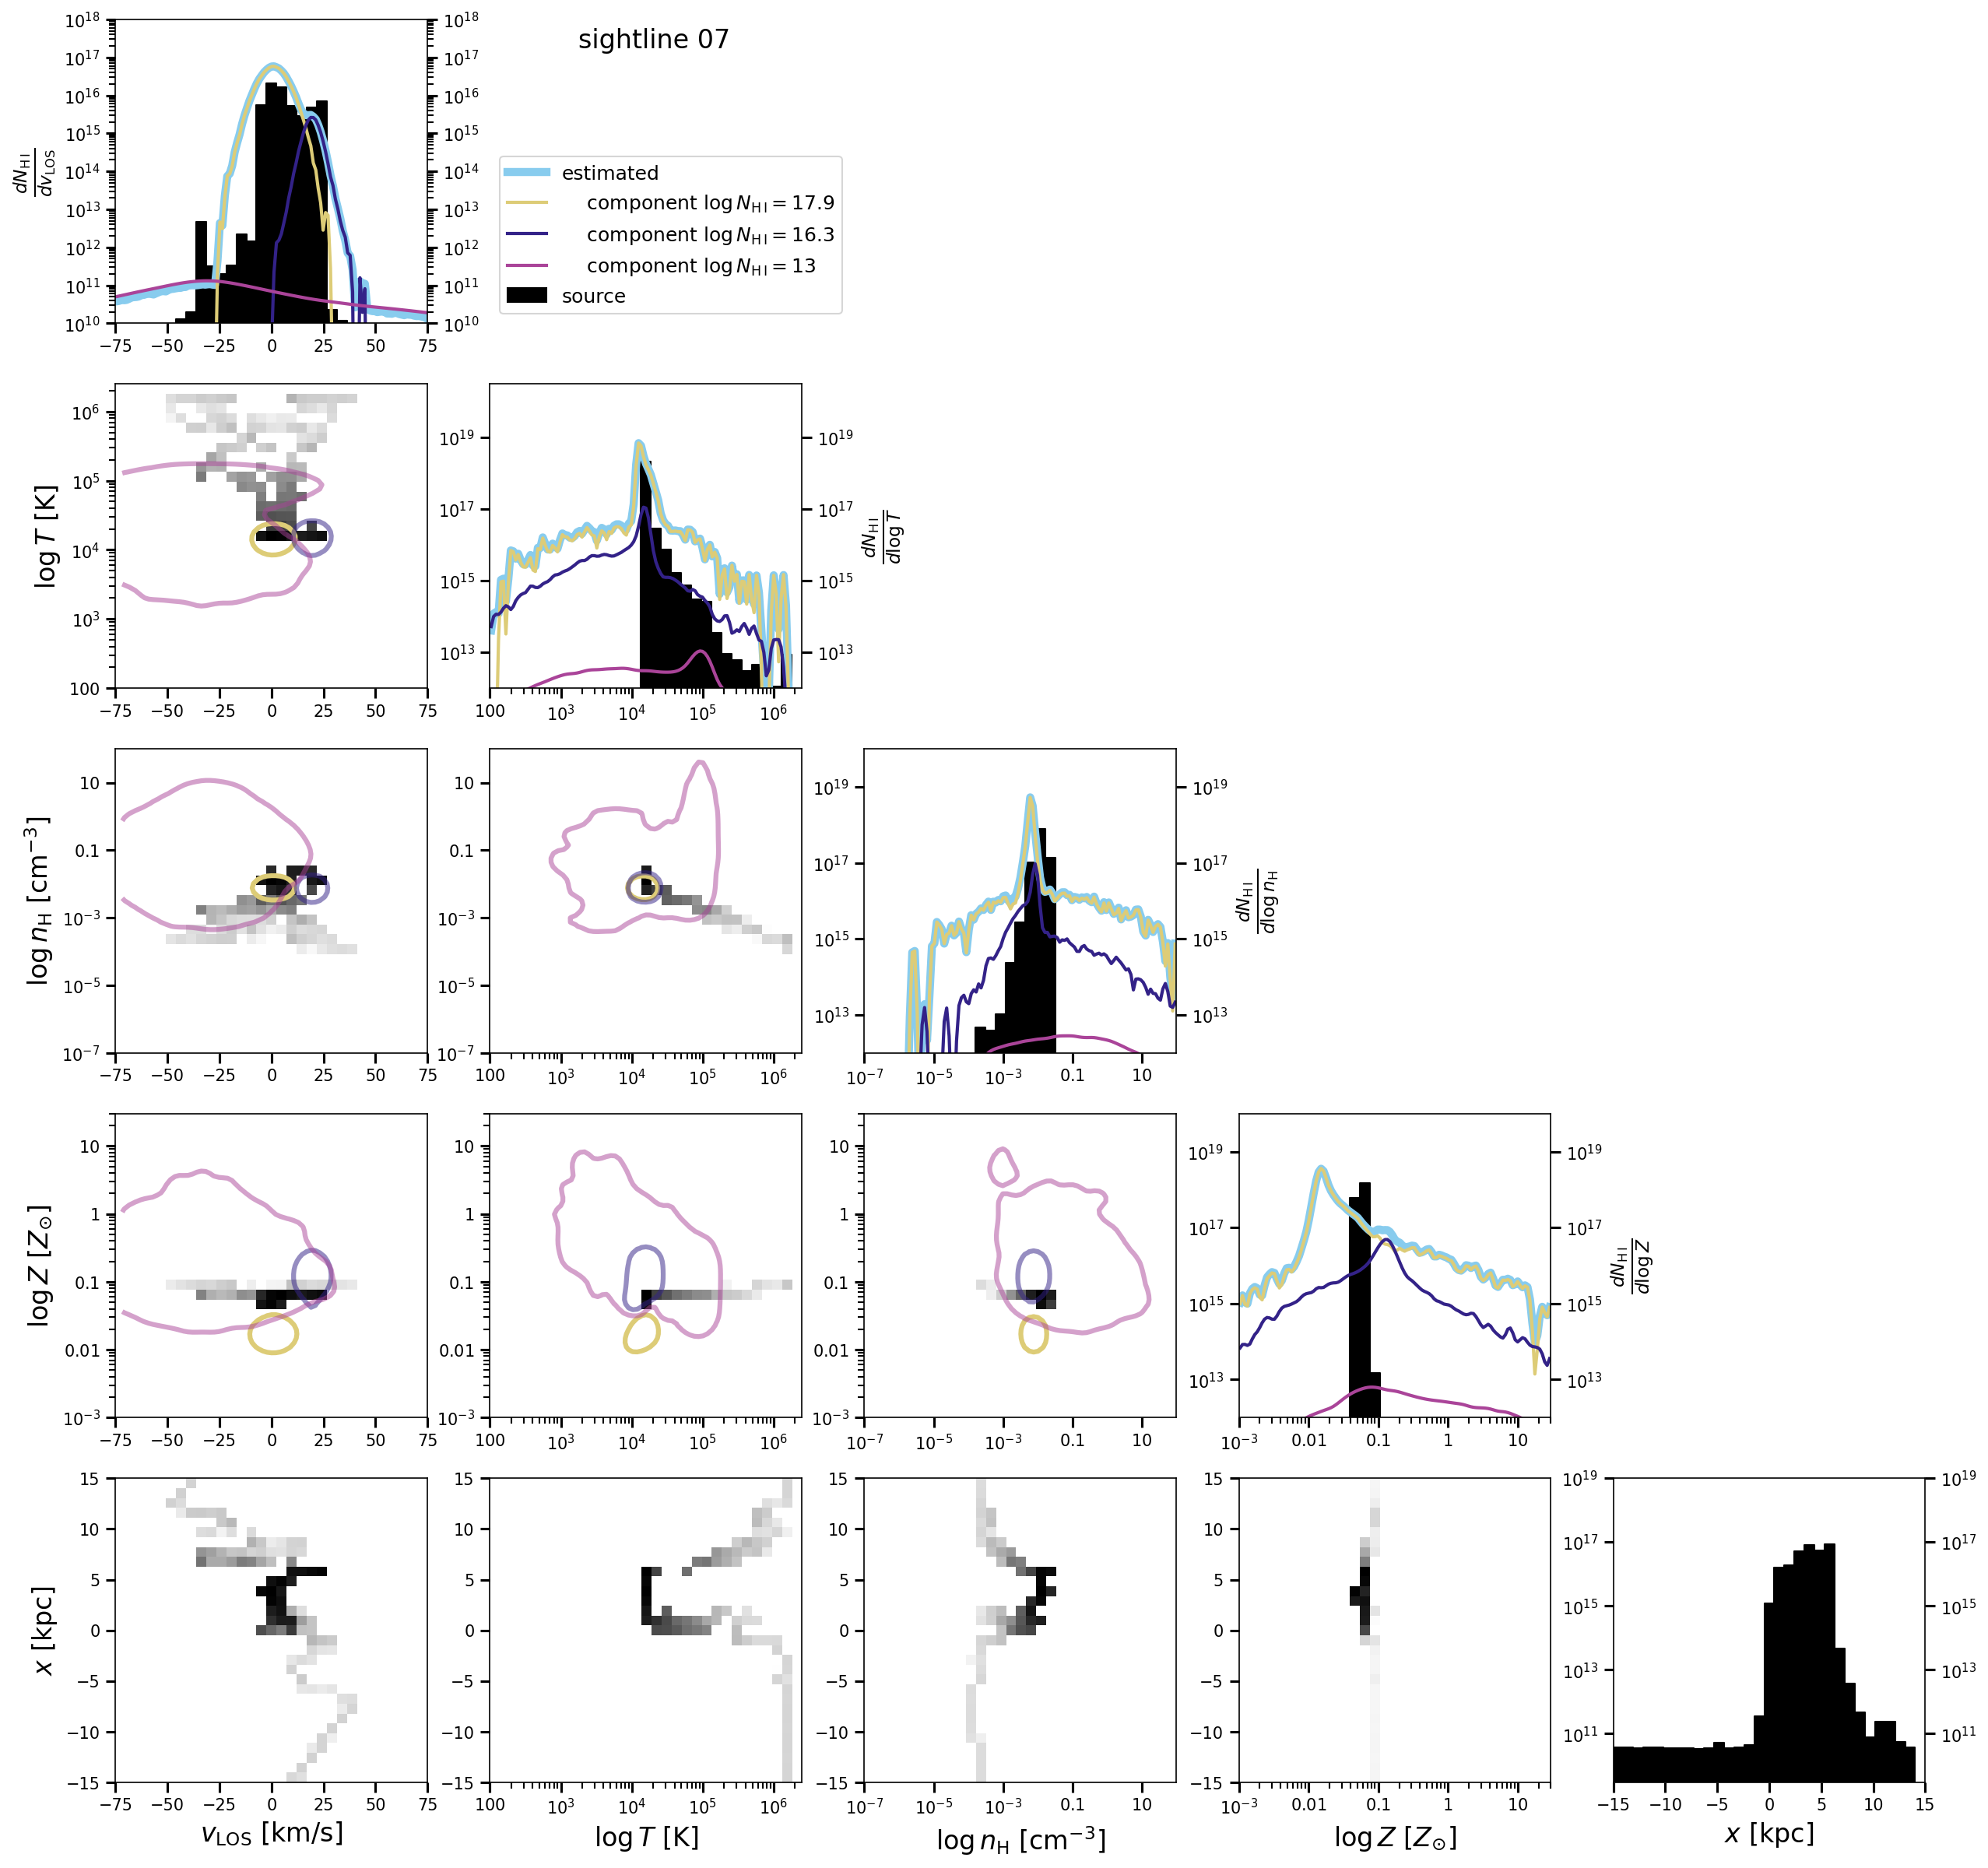
\includegraphics[height=0.45\textheight]{figures/sample2/high-z/sightline_0007.png}
    \label{f: sample2 07 corner}
    \caption{Same as Fig.~\ref{f: sample2 03}, but for sightline 07.}
\end{figure*}

\begin{figure*}
    \centering
    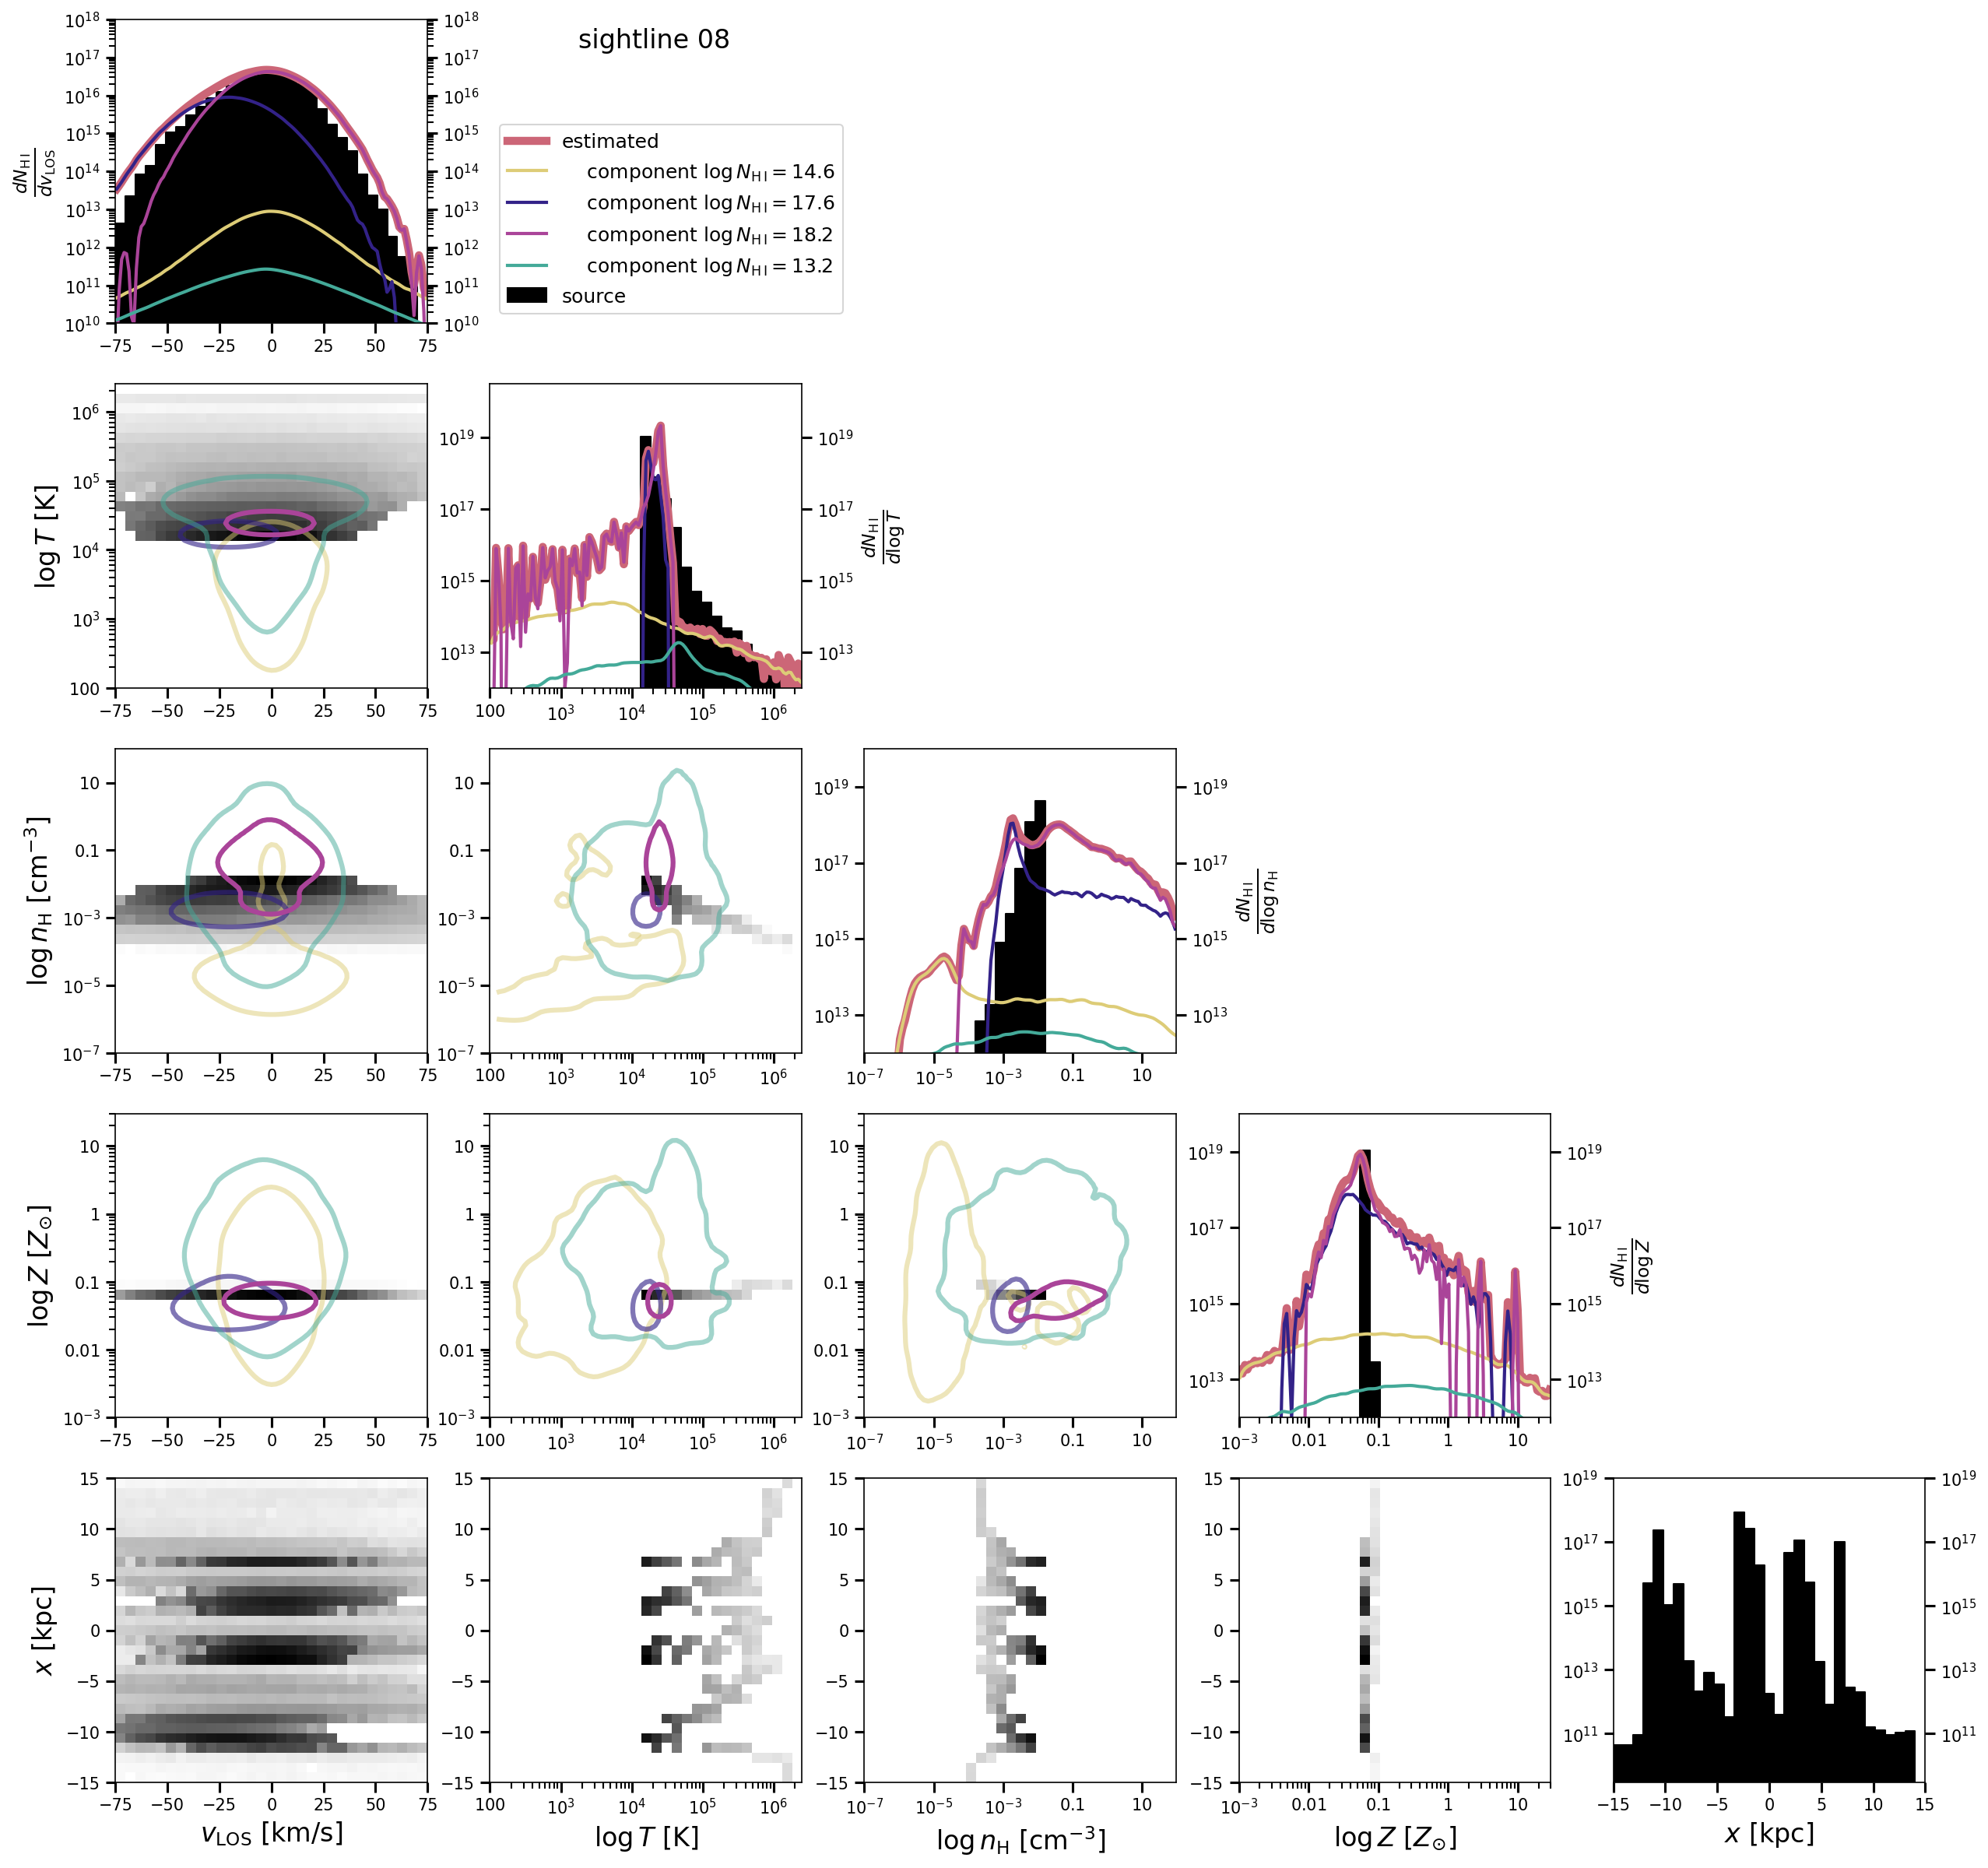
\includegraphics[height=0.45\textheight]{figures/sample2/original/sightline_0008.png}
    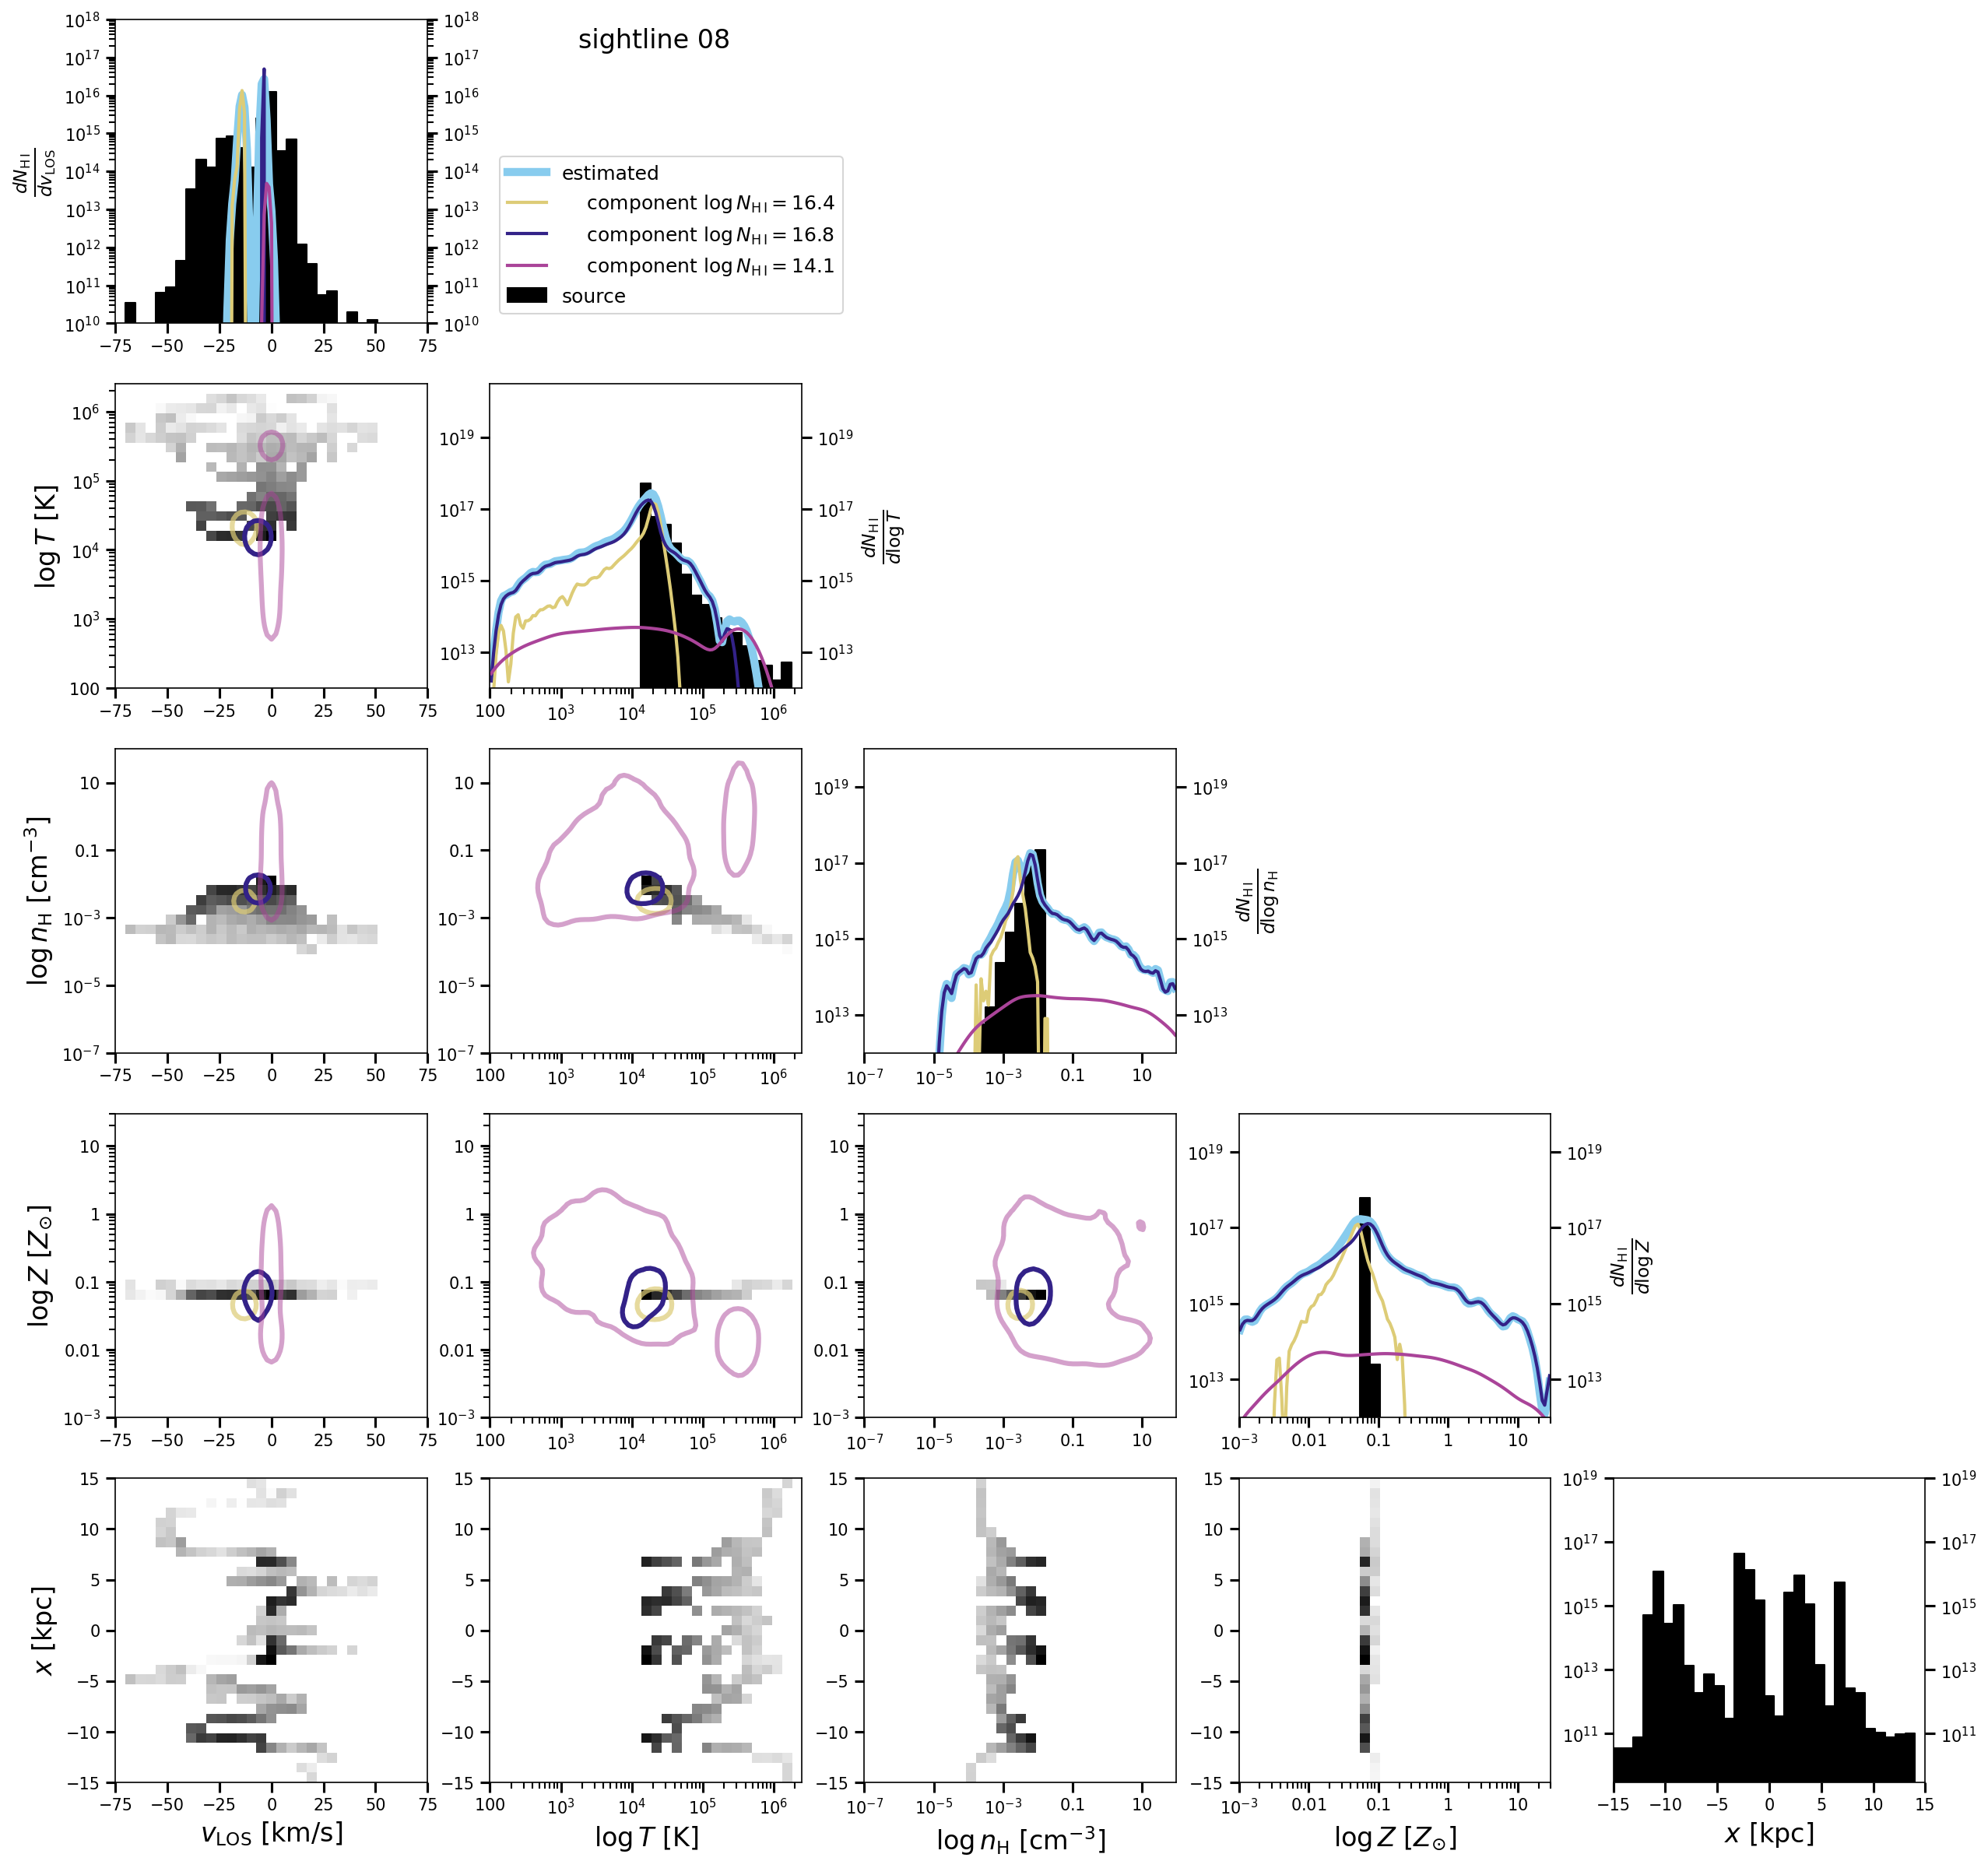
\includegraphics[height=0.45\textheight]{figures/sample2/high-z/sightline_0008.png}
    \label{f: sample2 08 corner}
    \caption{Same as Fig.~\ref{f: sample2 03}, but for sightline 08.}
\end{figure*}

\begin{figure*}
    \centering
    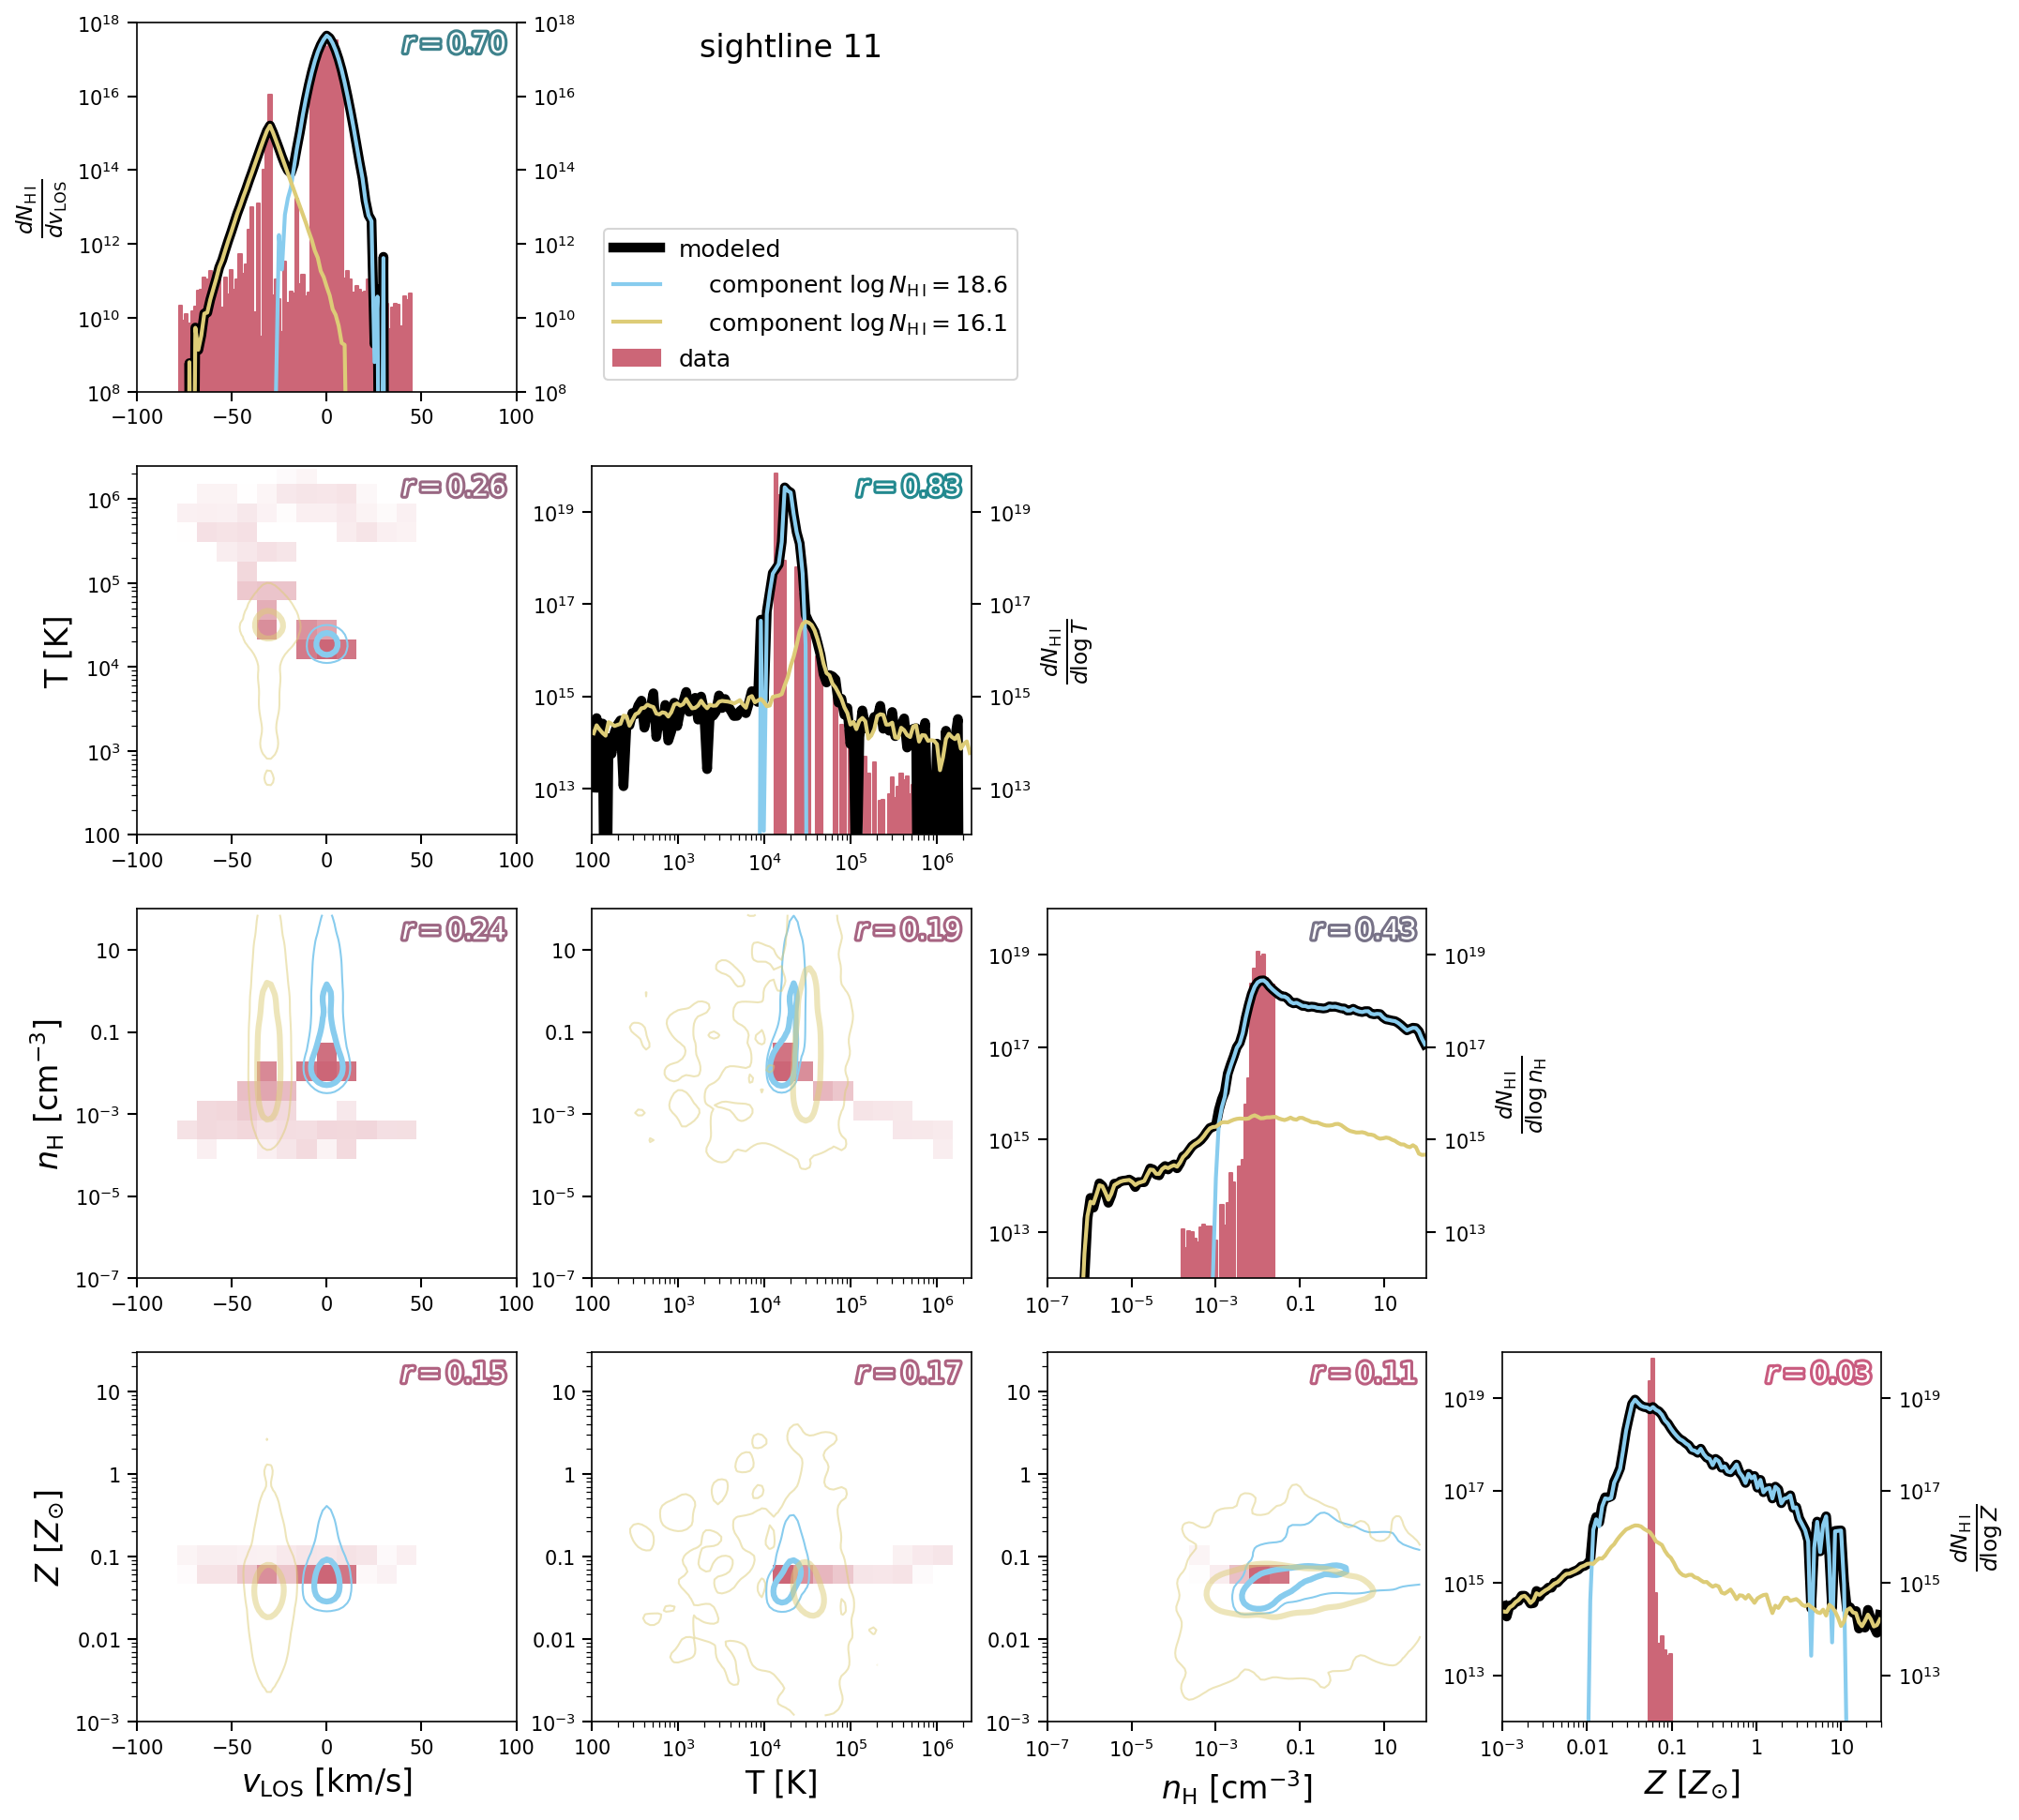
\includegraphics[height=0.45\textheight]{figures/sample2/original/sightline_0011.png}
    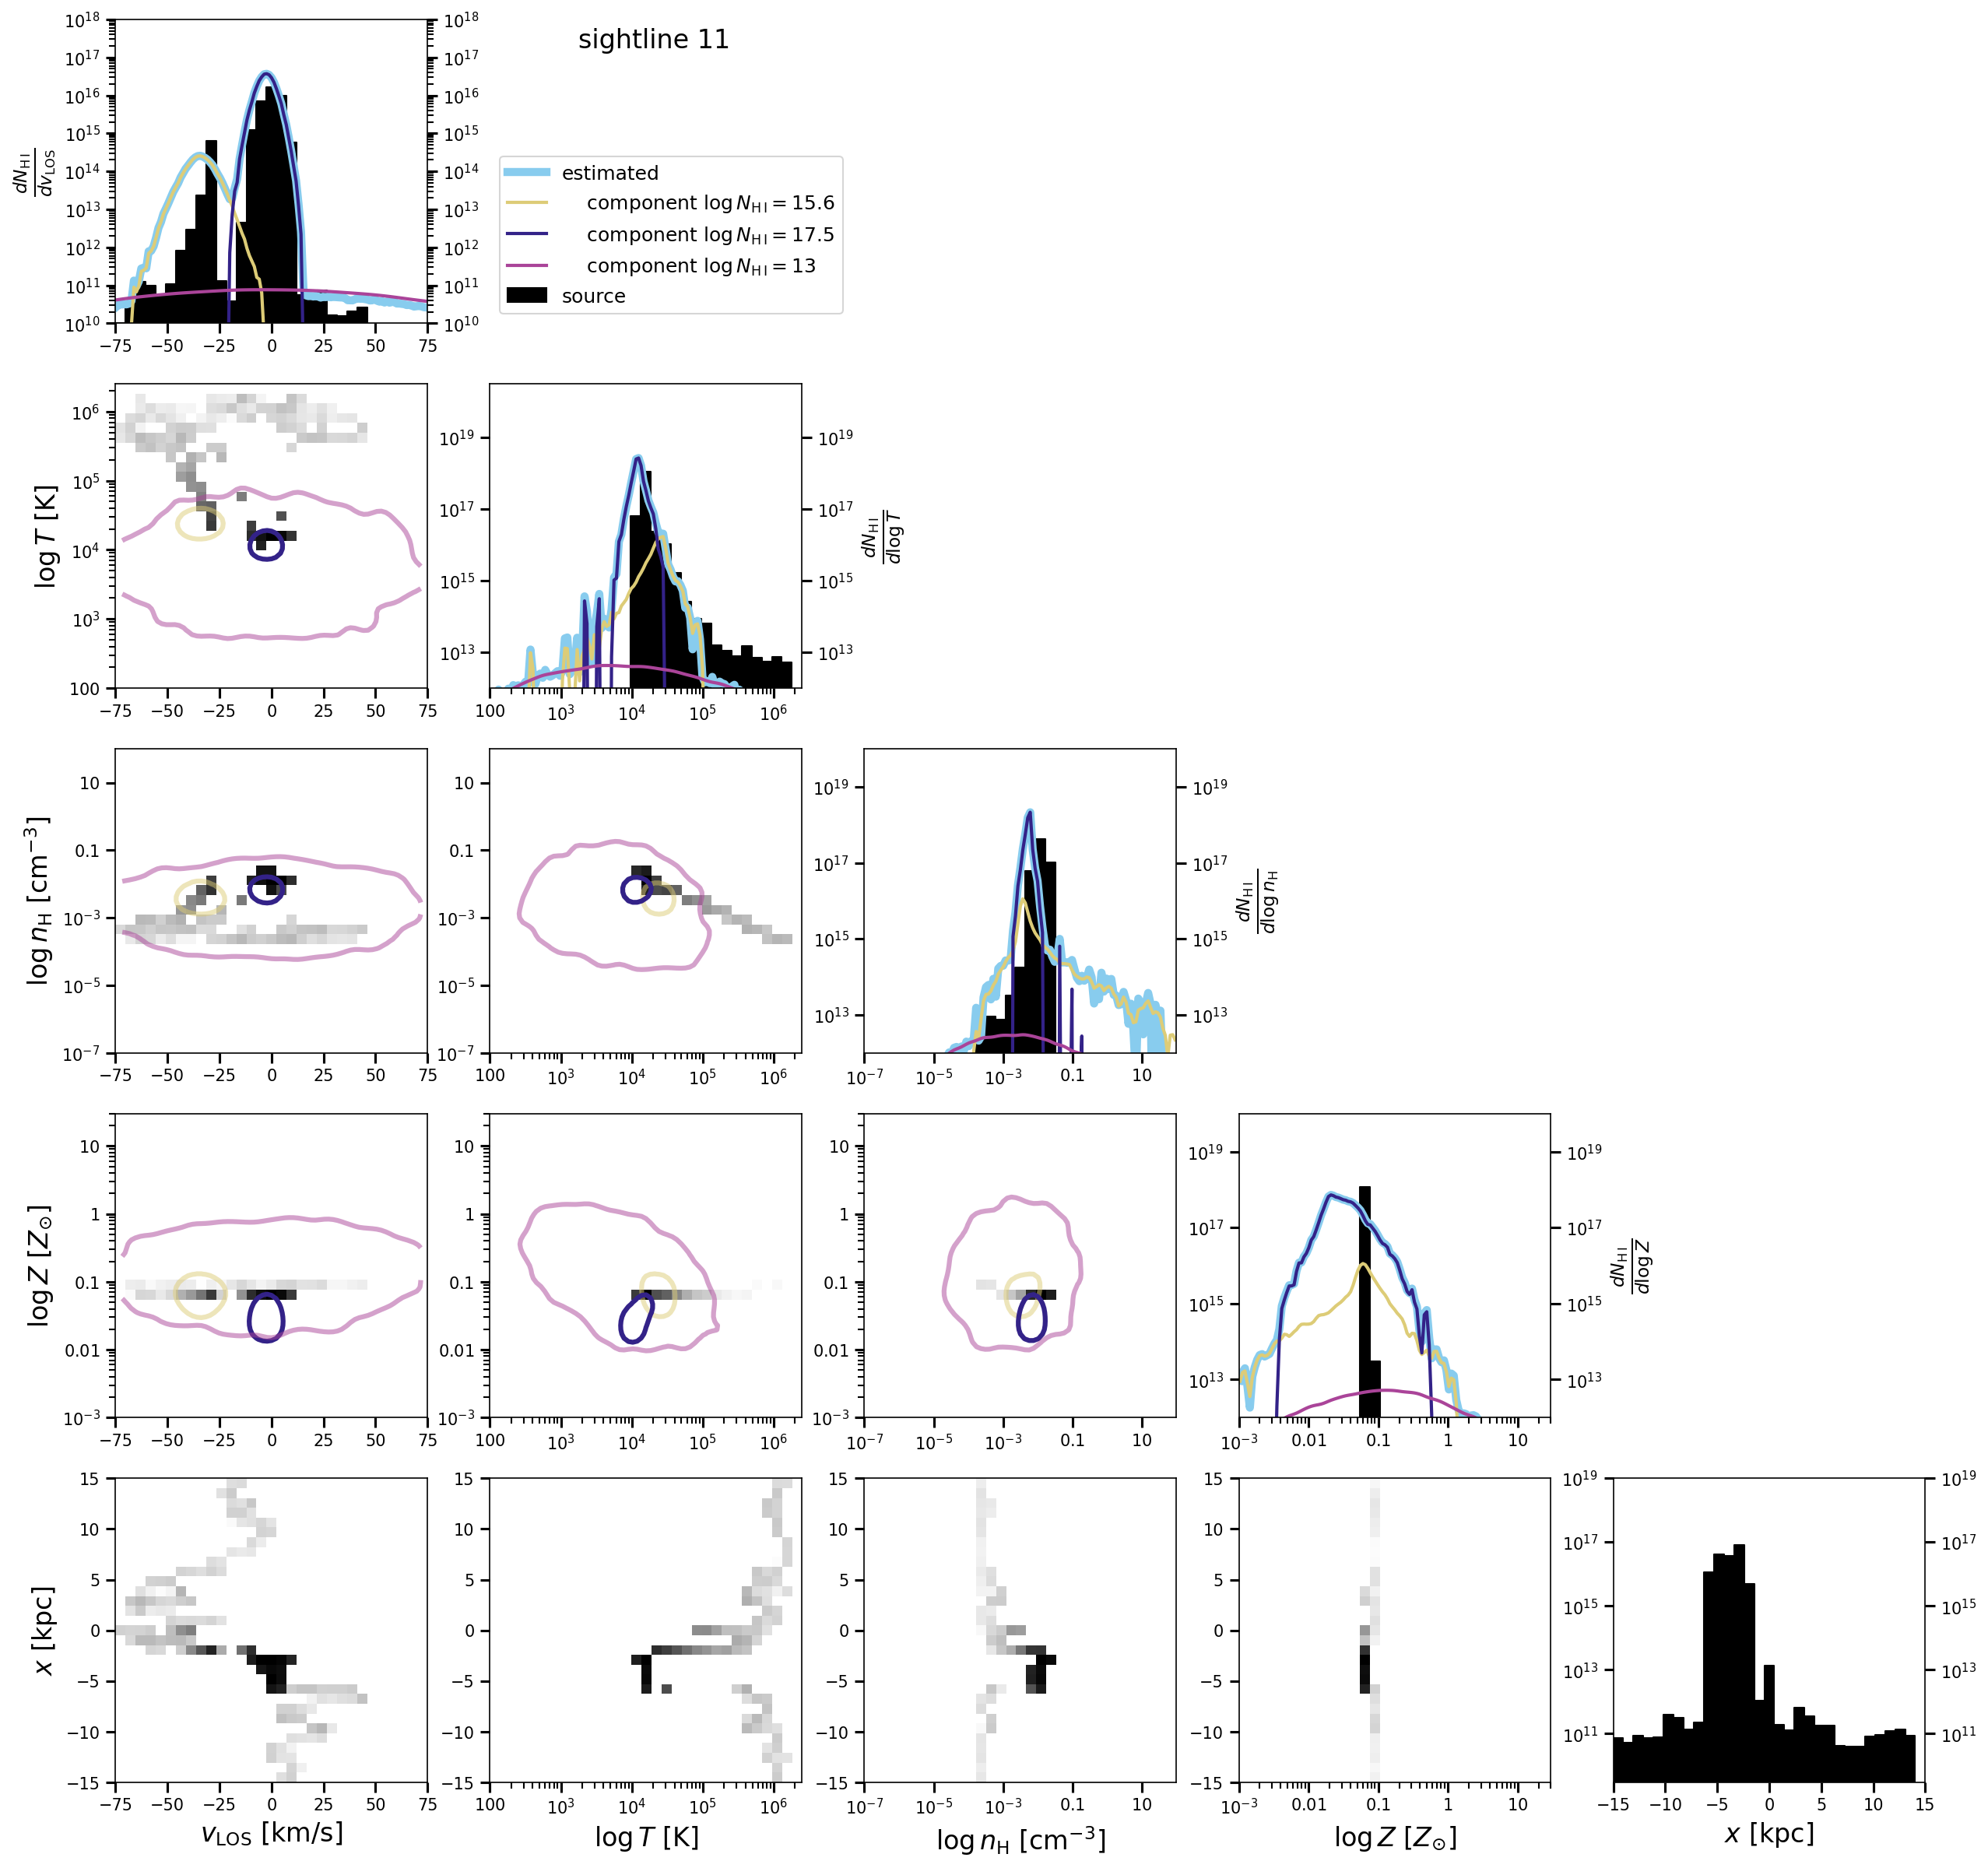
\includegraphics[height=0.45\textheight]{figures/sample2/high-z/sightline_0011.png}
    \label{f: sample2 11 corner}
    \caption{Same as Fig.~\ref{f: sample2 03}, but for sightline 11.}
\end{figure*}

\begin{figure*}
    \centering
    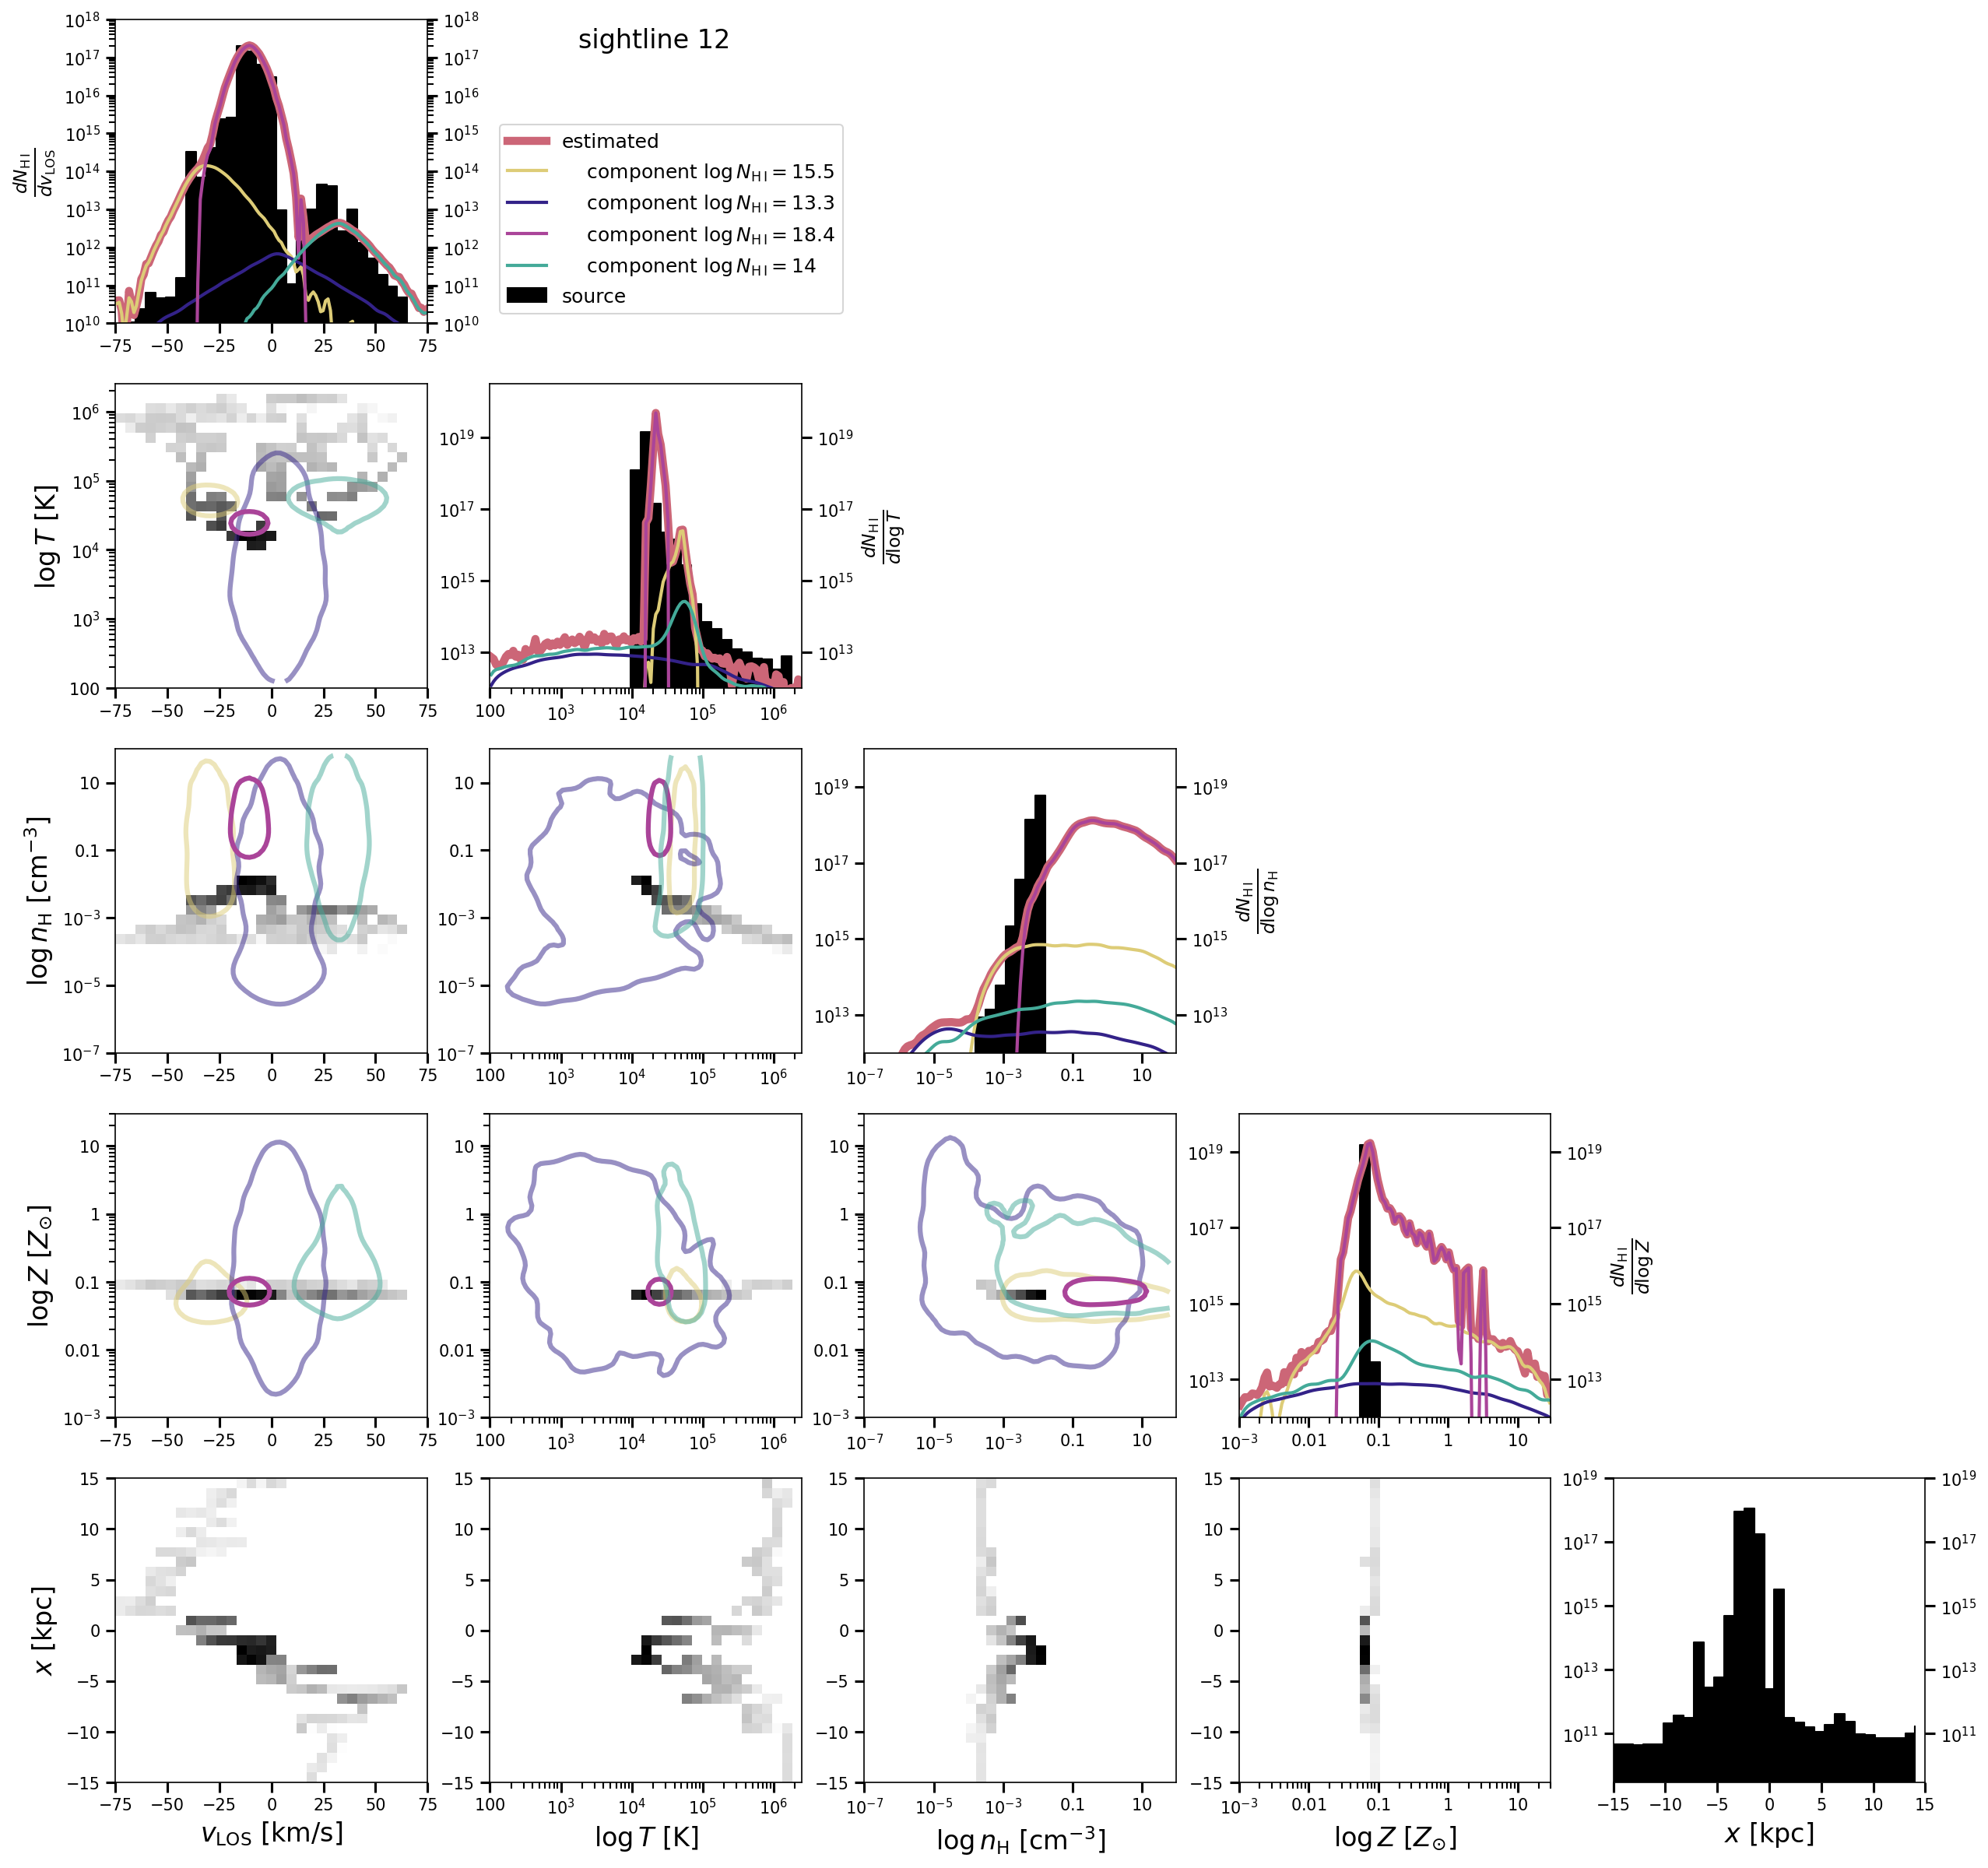
\includegraphics[height=0.45\textheight]{figures/sample2/original/sightline_0012.png}
    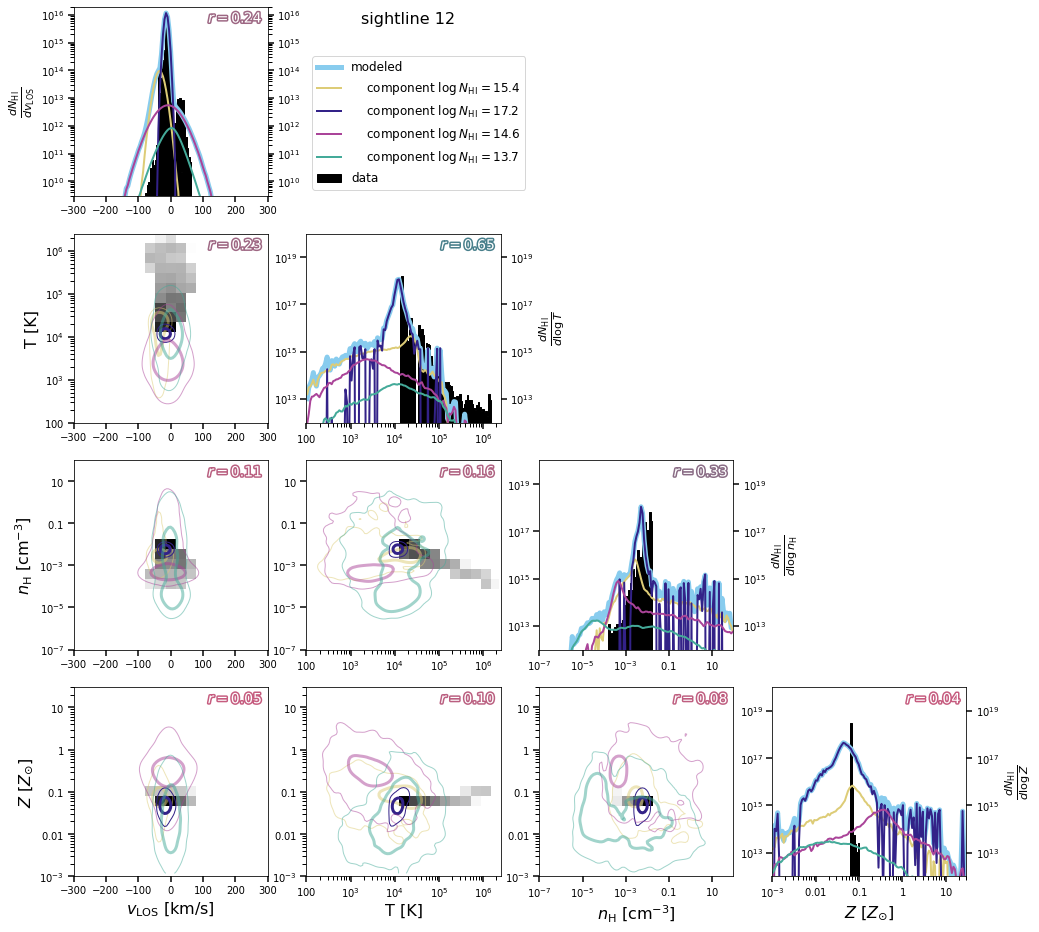
\includegraphics[height=0.45\textheight]{figures/sample2/high-z/sightline_0012.png}
    \label{f: sample2 12 corner}
    \caption{Same as Fig.~\ref{f: sample2 03}, but for sightline 12.}
\end{figure*}

\begin{figure*}
    \centering
    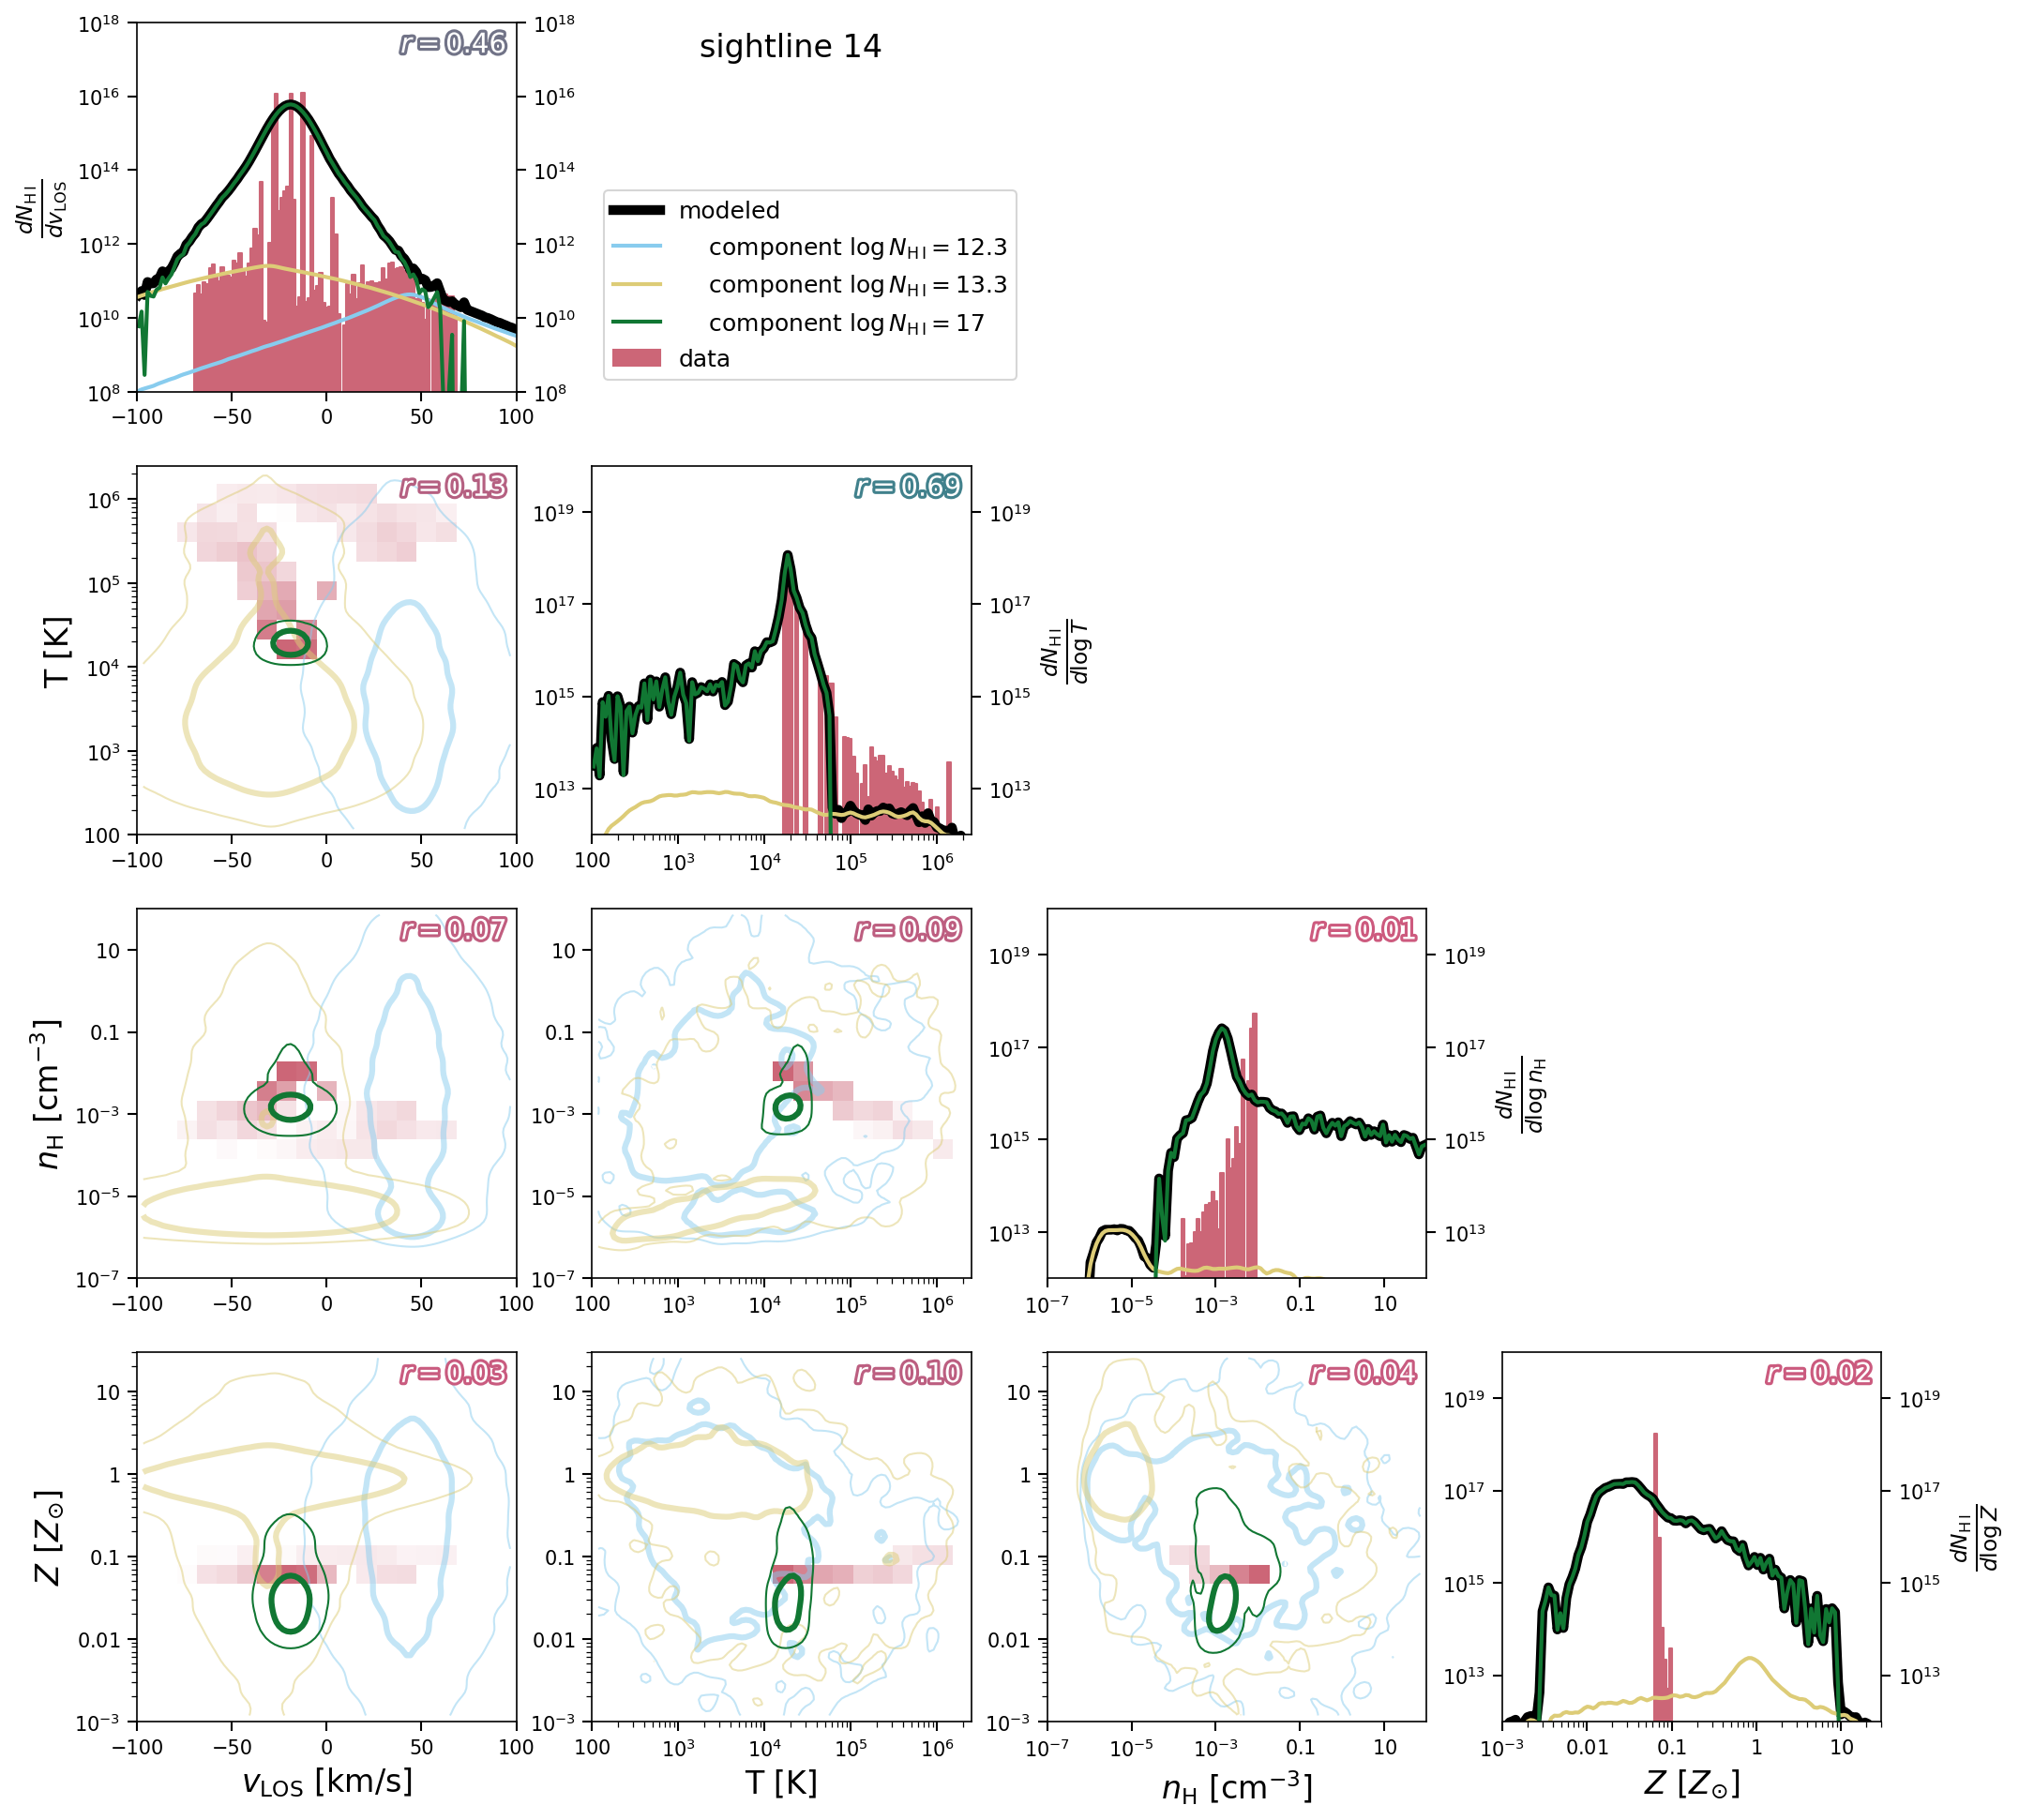
\includegraphics[height=0.45\textheight]{figures/sample2/original/sightline_0014.png}
    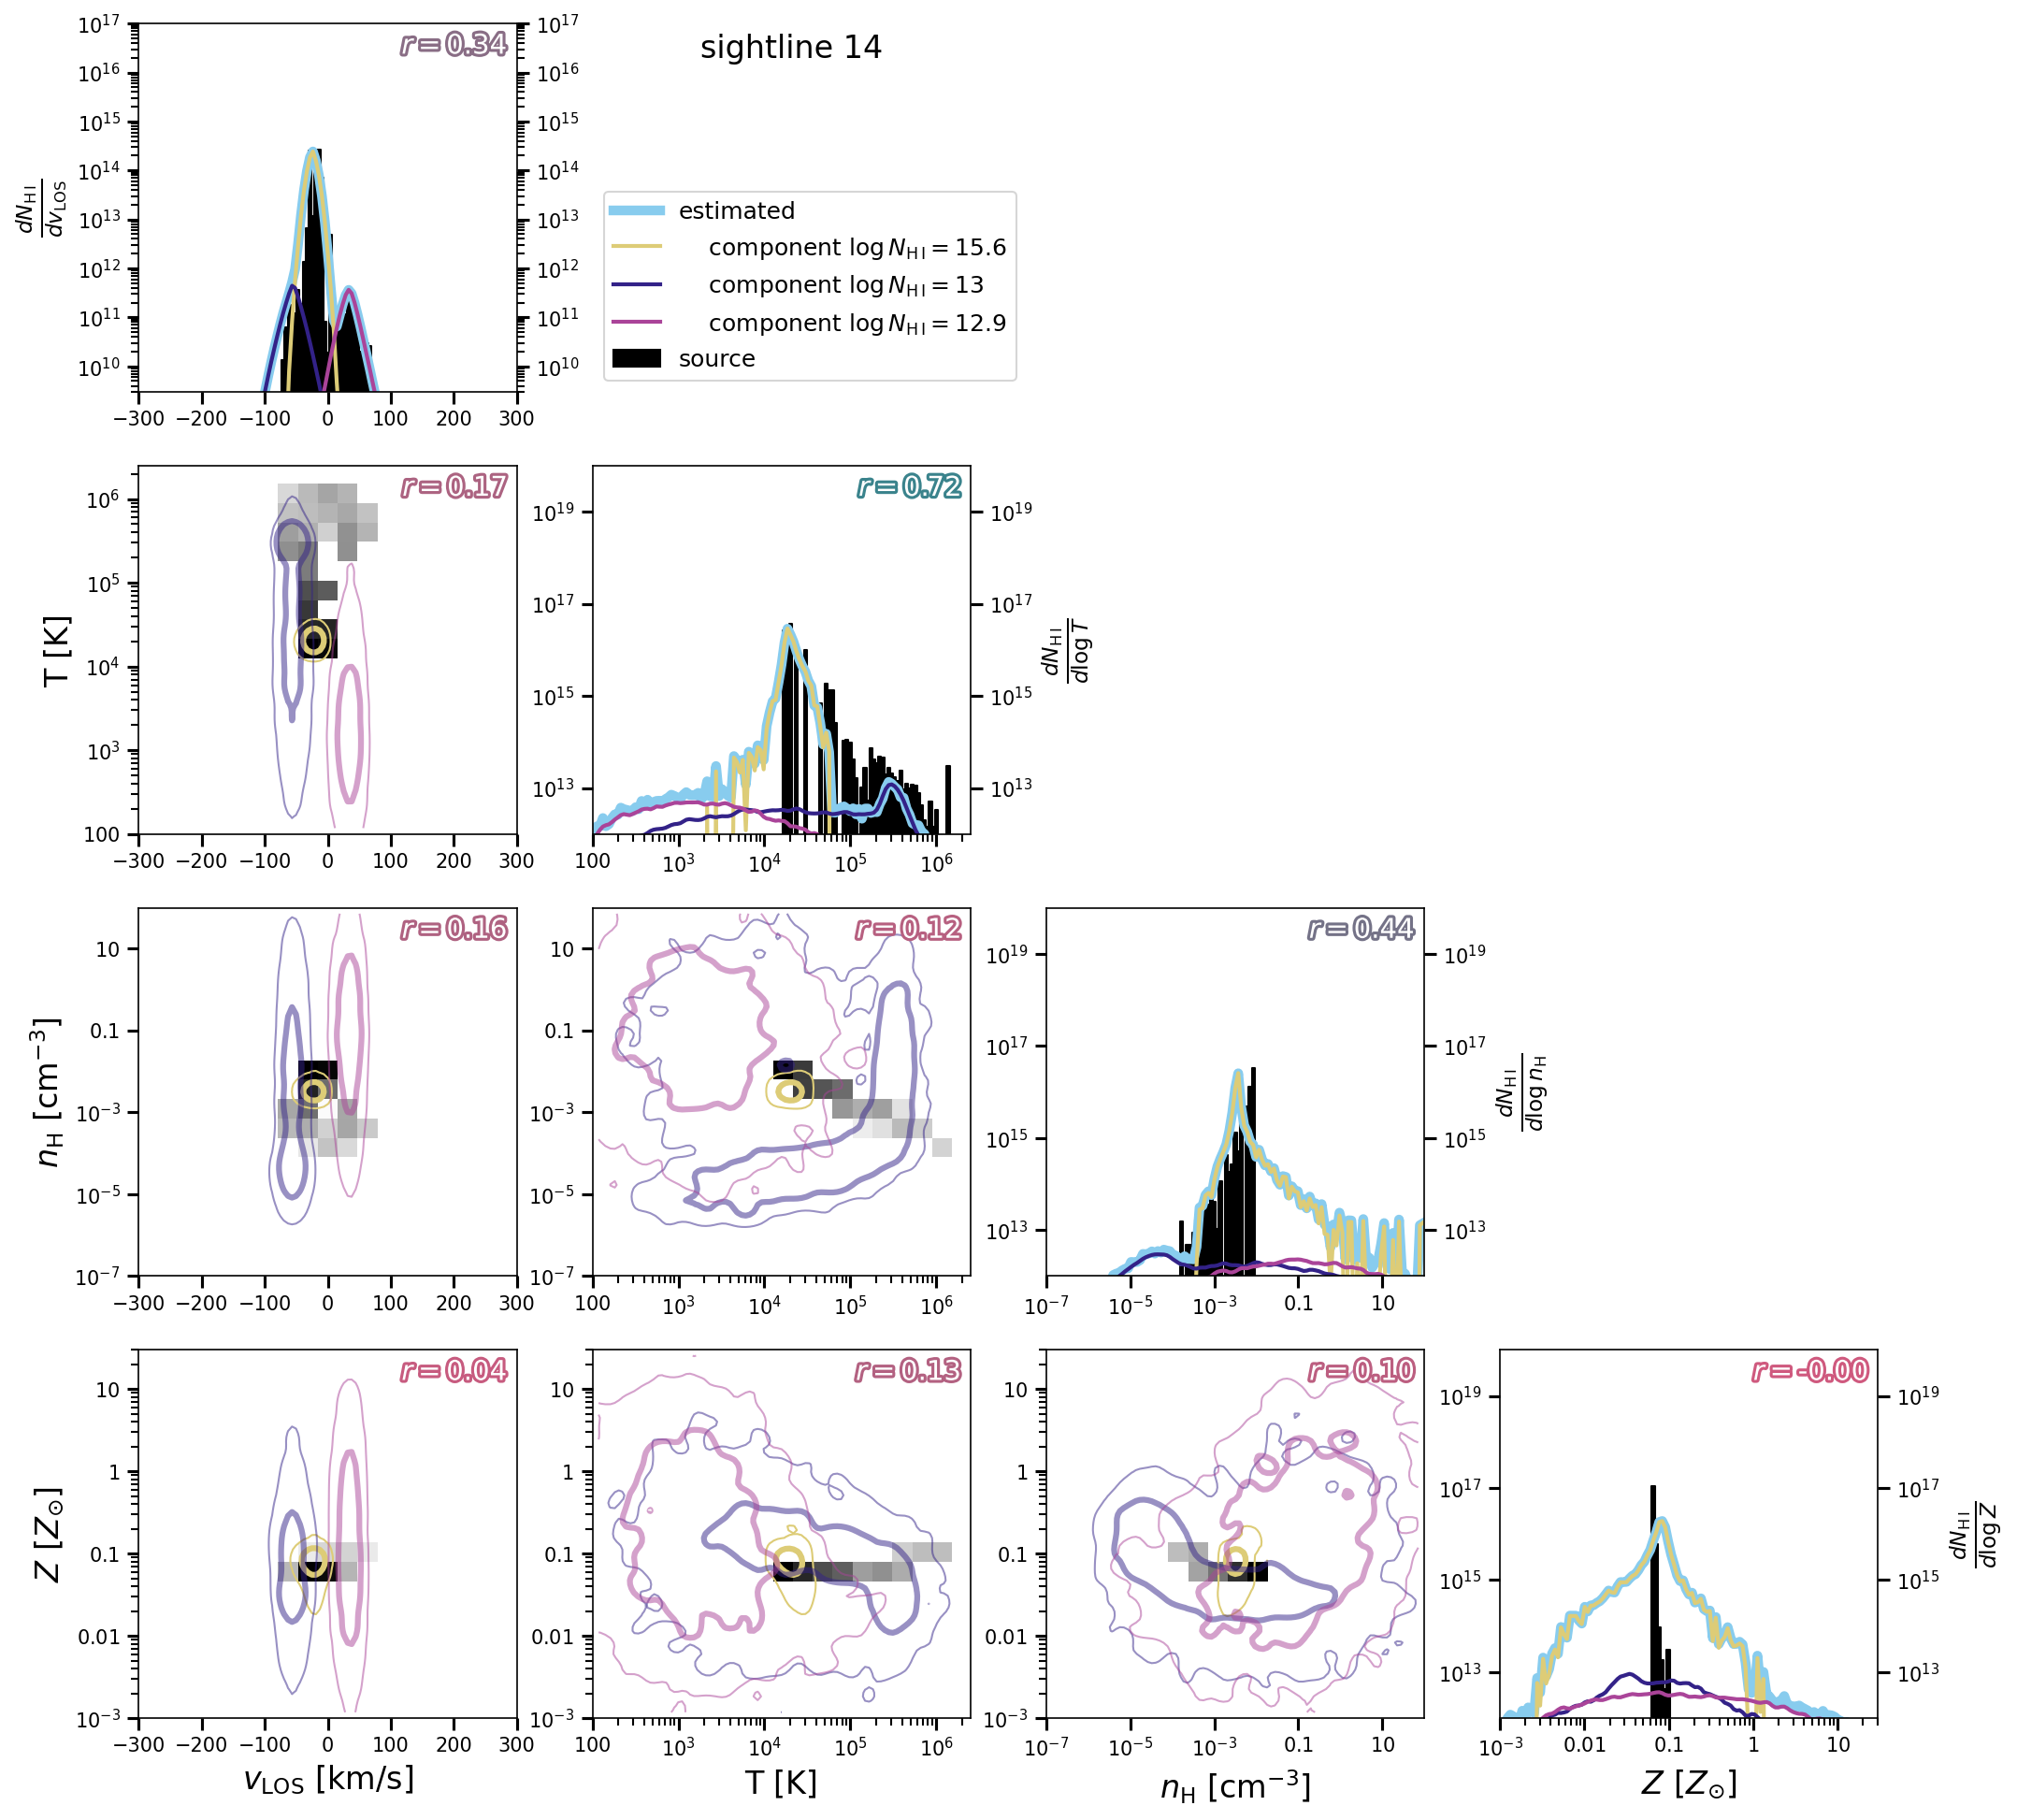
\includegraphics[height=0.45\textheight]{figures/sample2/high-z/sightline_0014.png}
    \label{f: sample2 14 corner}
    \caption{Same as Fig.~\ref{f: sample2 03}, but for sightline 14.}
\end{figure*}

\begin{figure*}
    \centering
    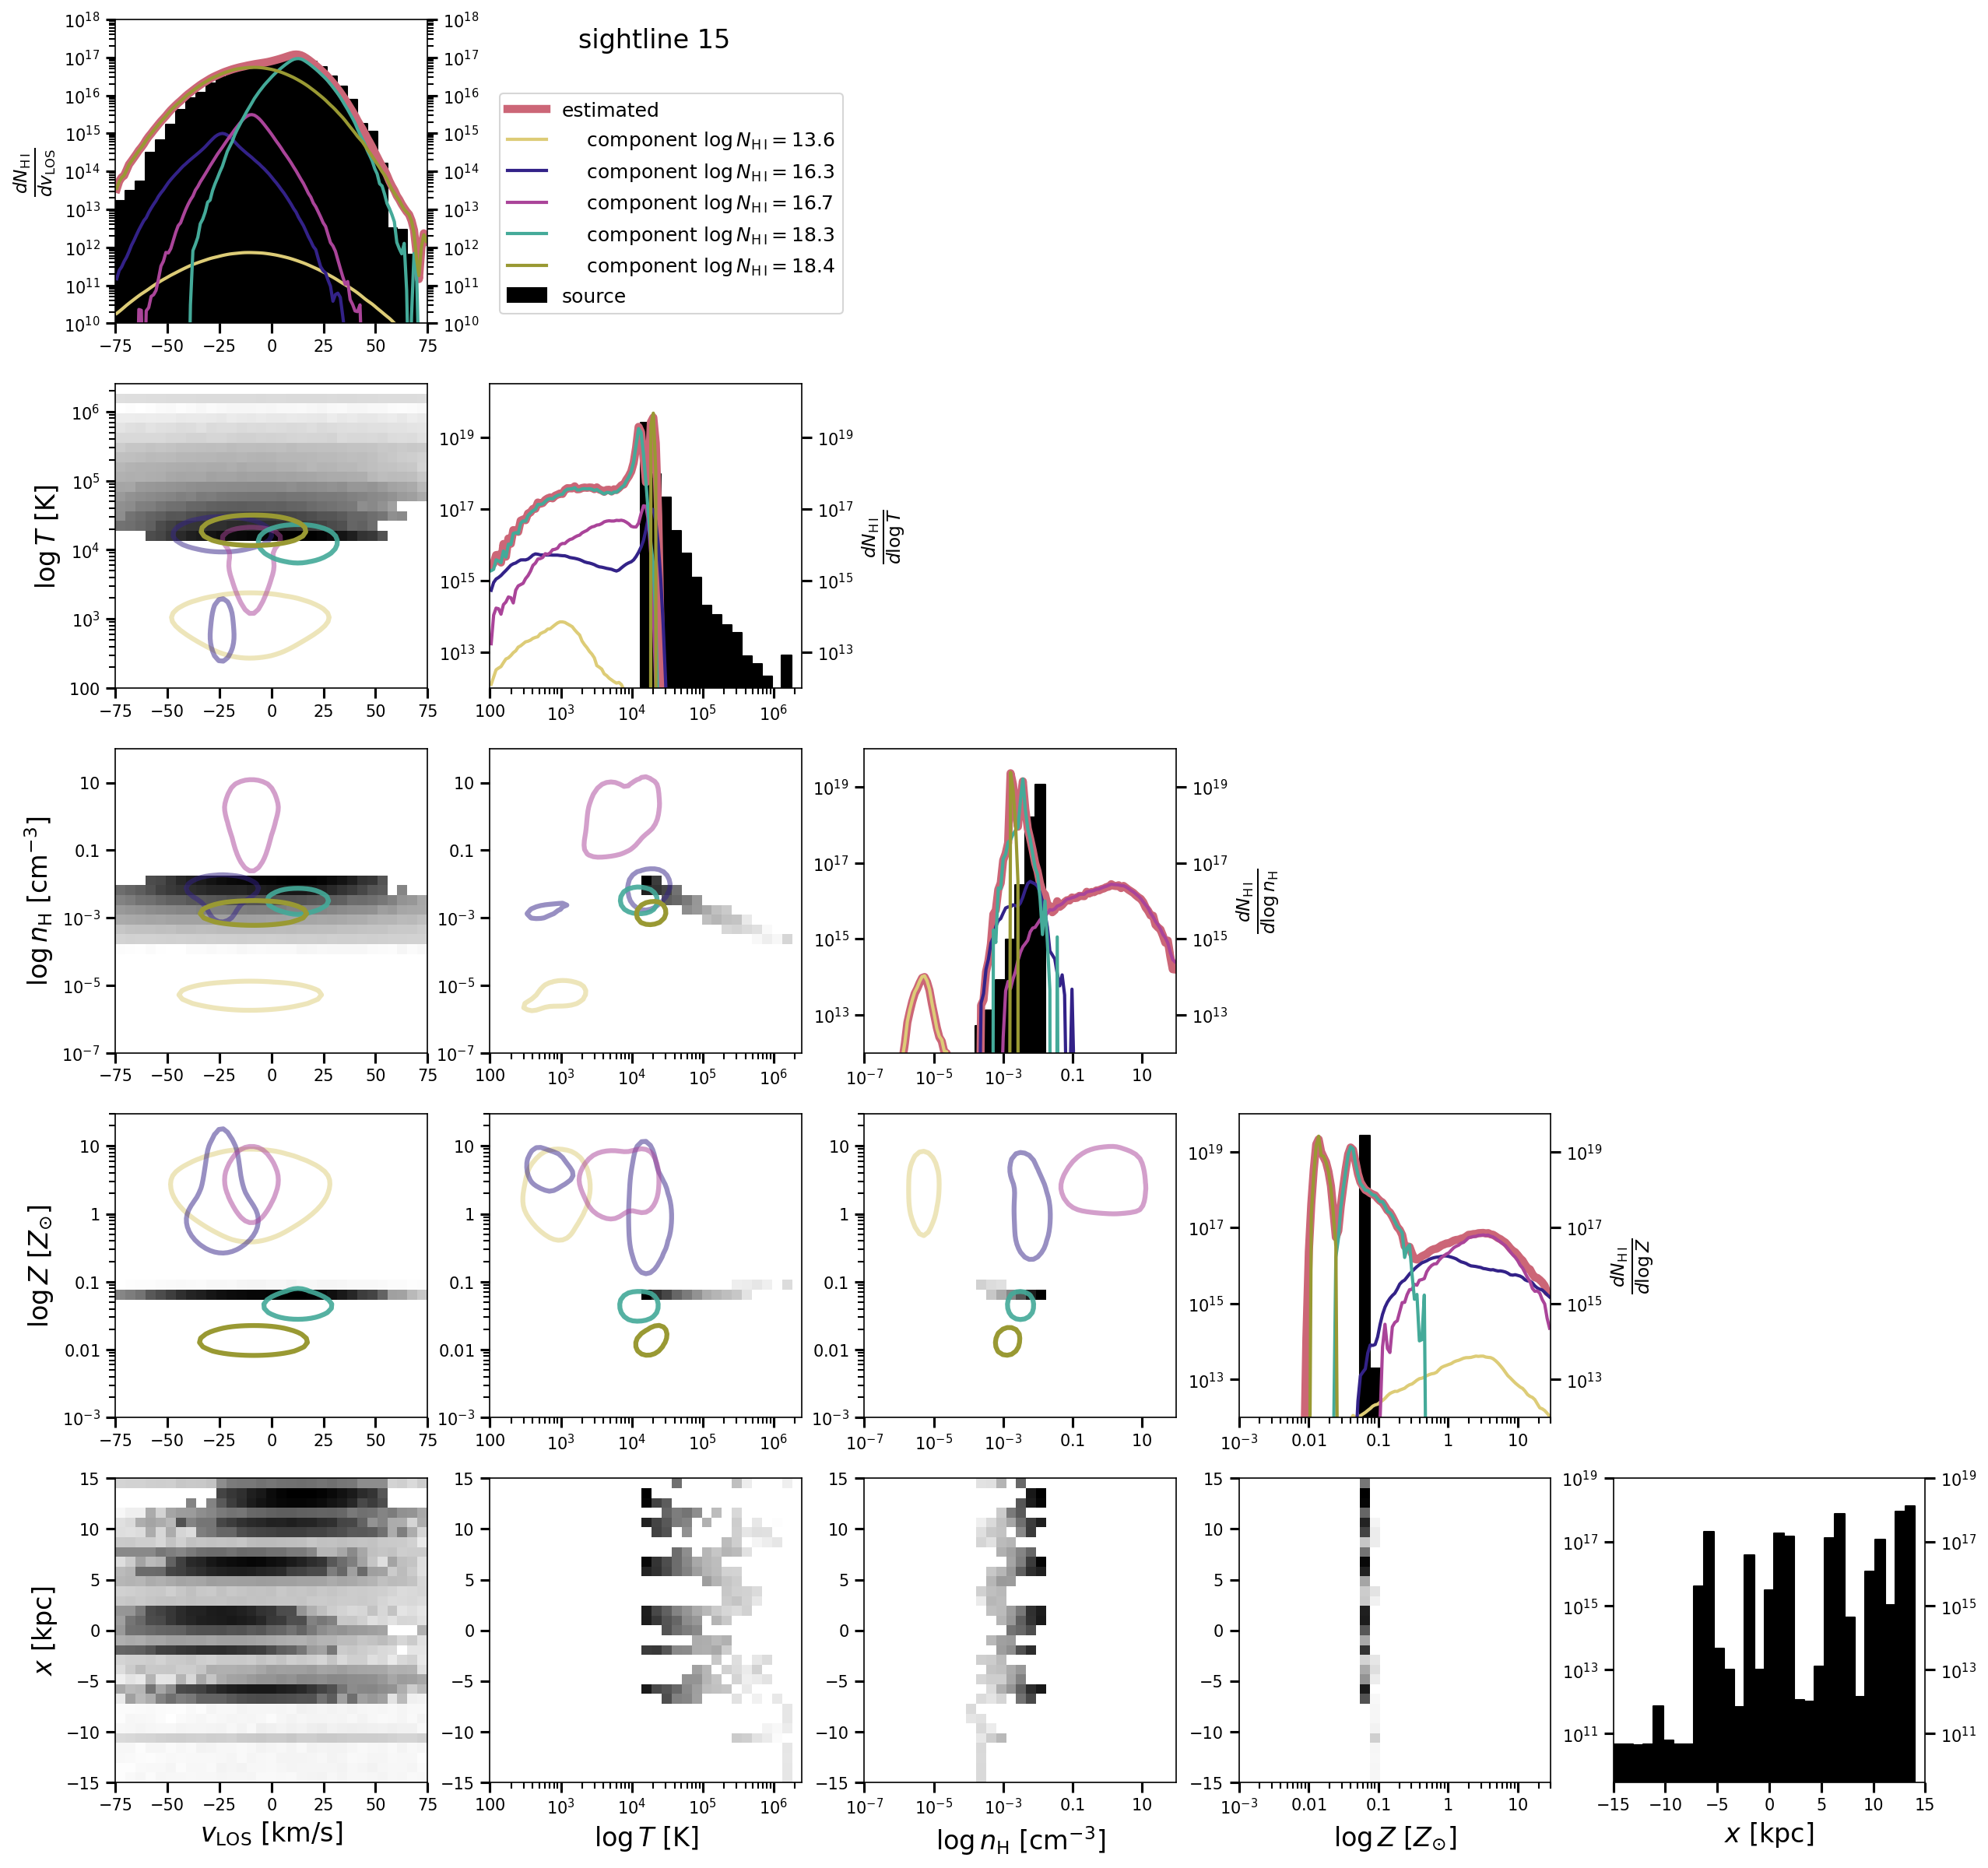
\includegraphics[height=0.45\textheight]{figures/sample2/original/sightline_0015.png}
    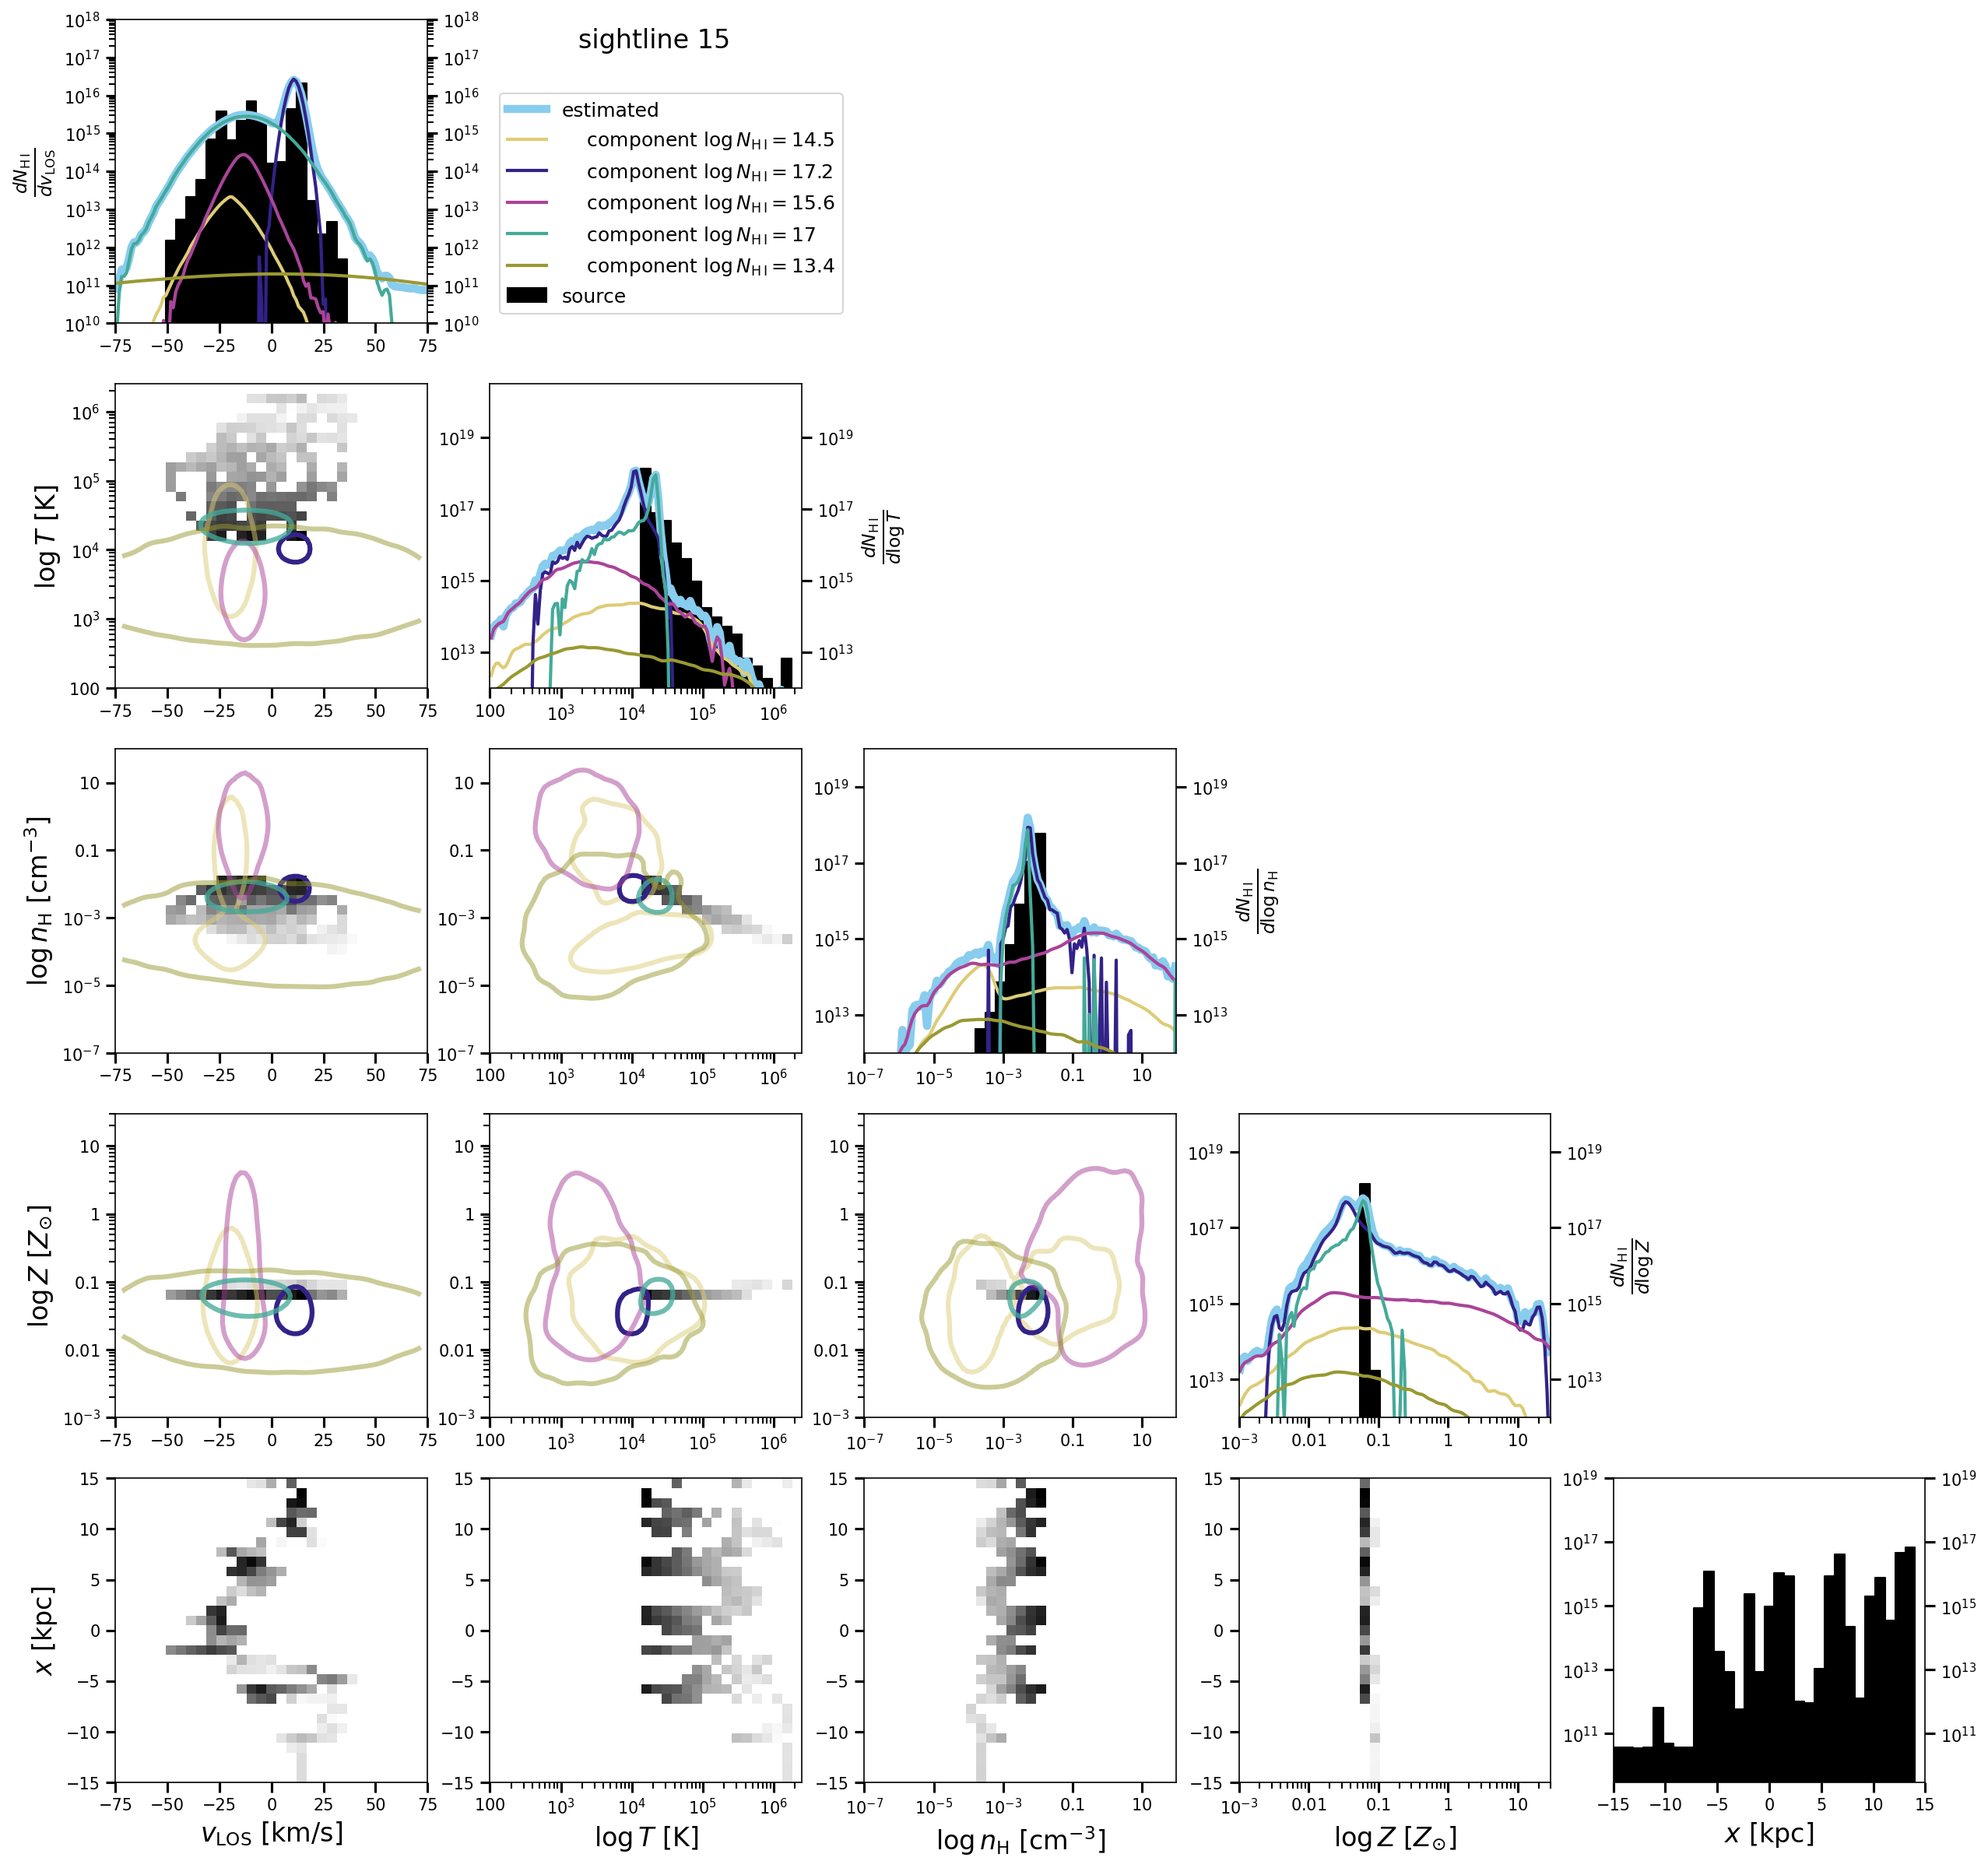
\includegraphics[height=0.45\textheight]{figures/sample2/high-z/sightline_0015.png}
    \label{f: sample2 15 corner}
    \caption{Same as Fig.~\ref{f: sample2 03}, but for sightline 15.}
\end{figure*}

\begin{figure*}
    \centering
    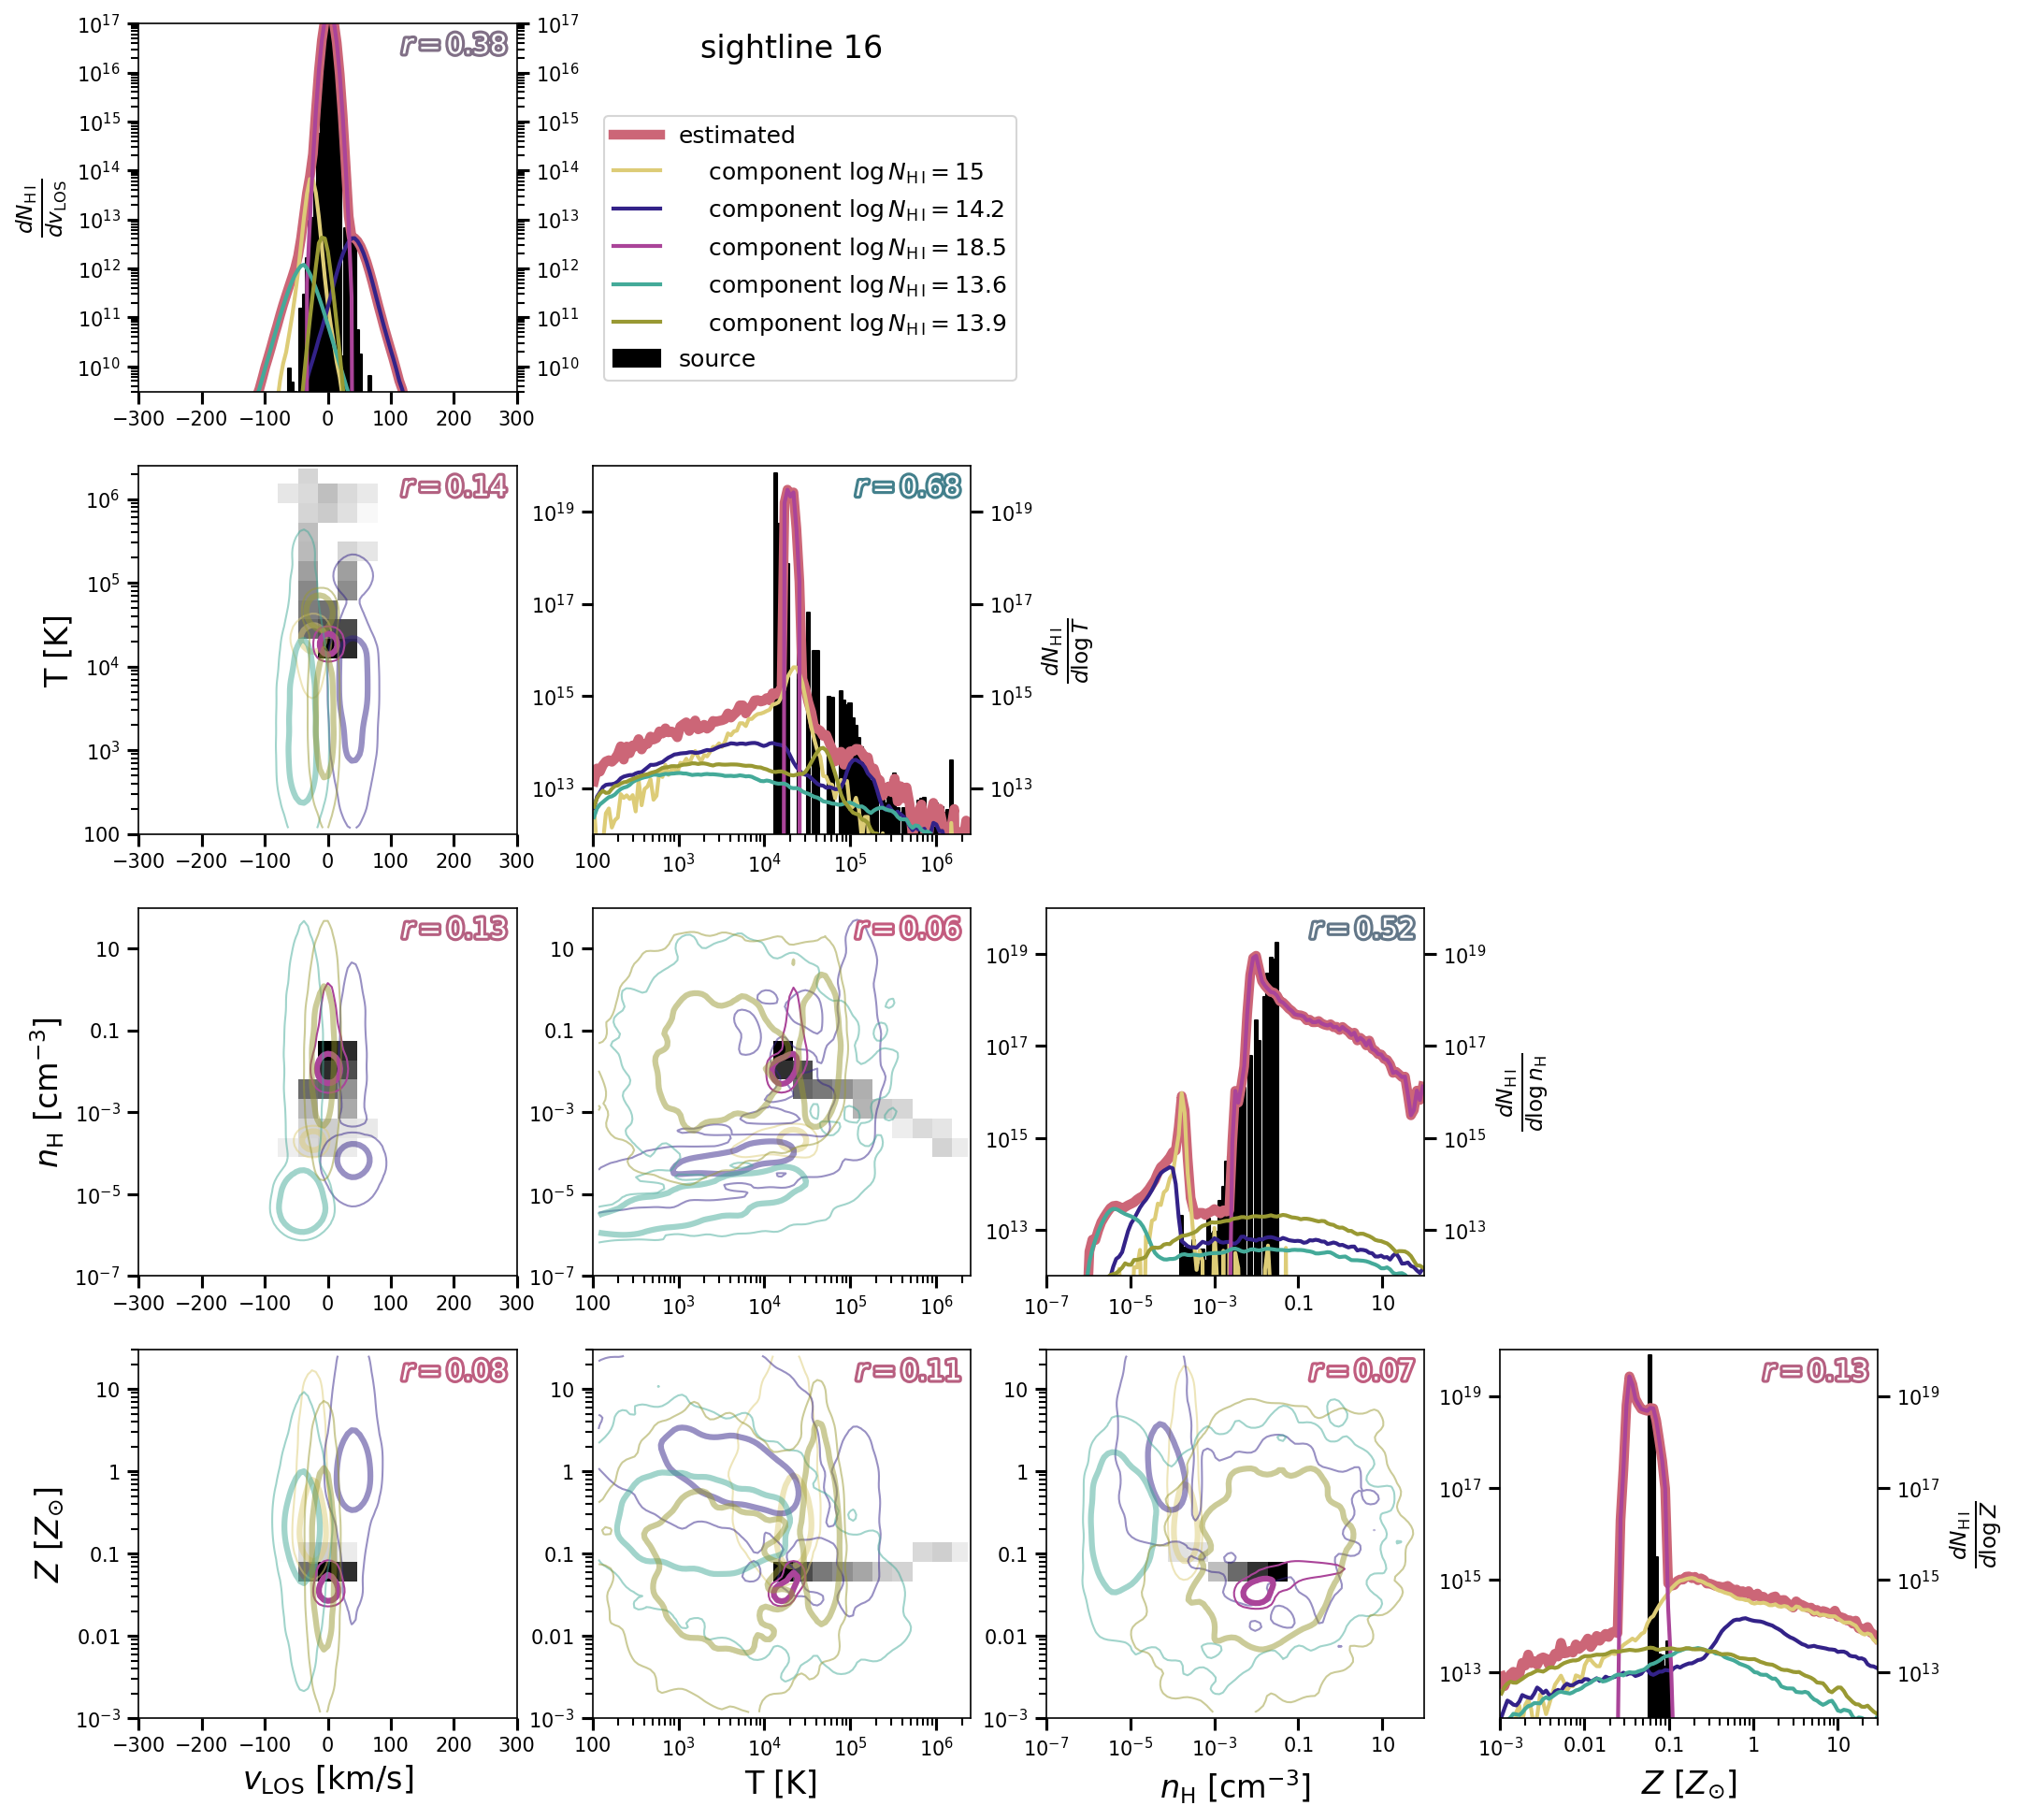
\includegraphics[height=0.45\textheight]{figures/sample2/original/sightline_0016.png}
    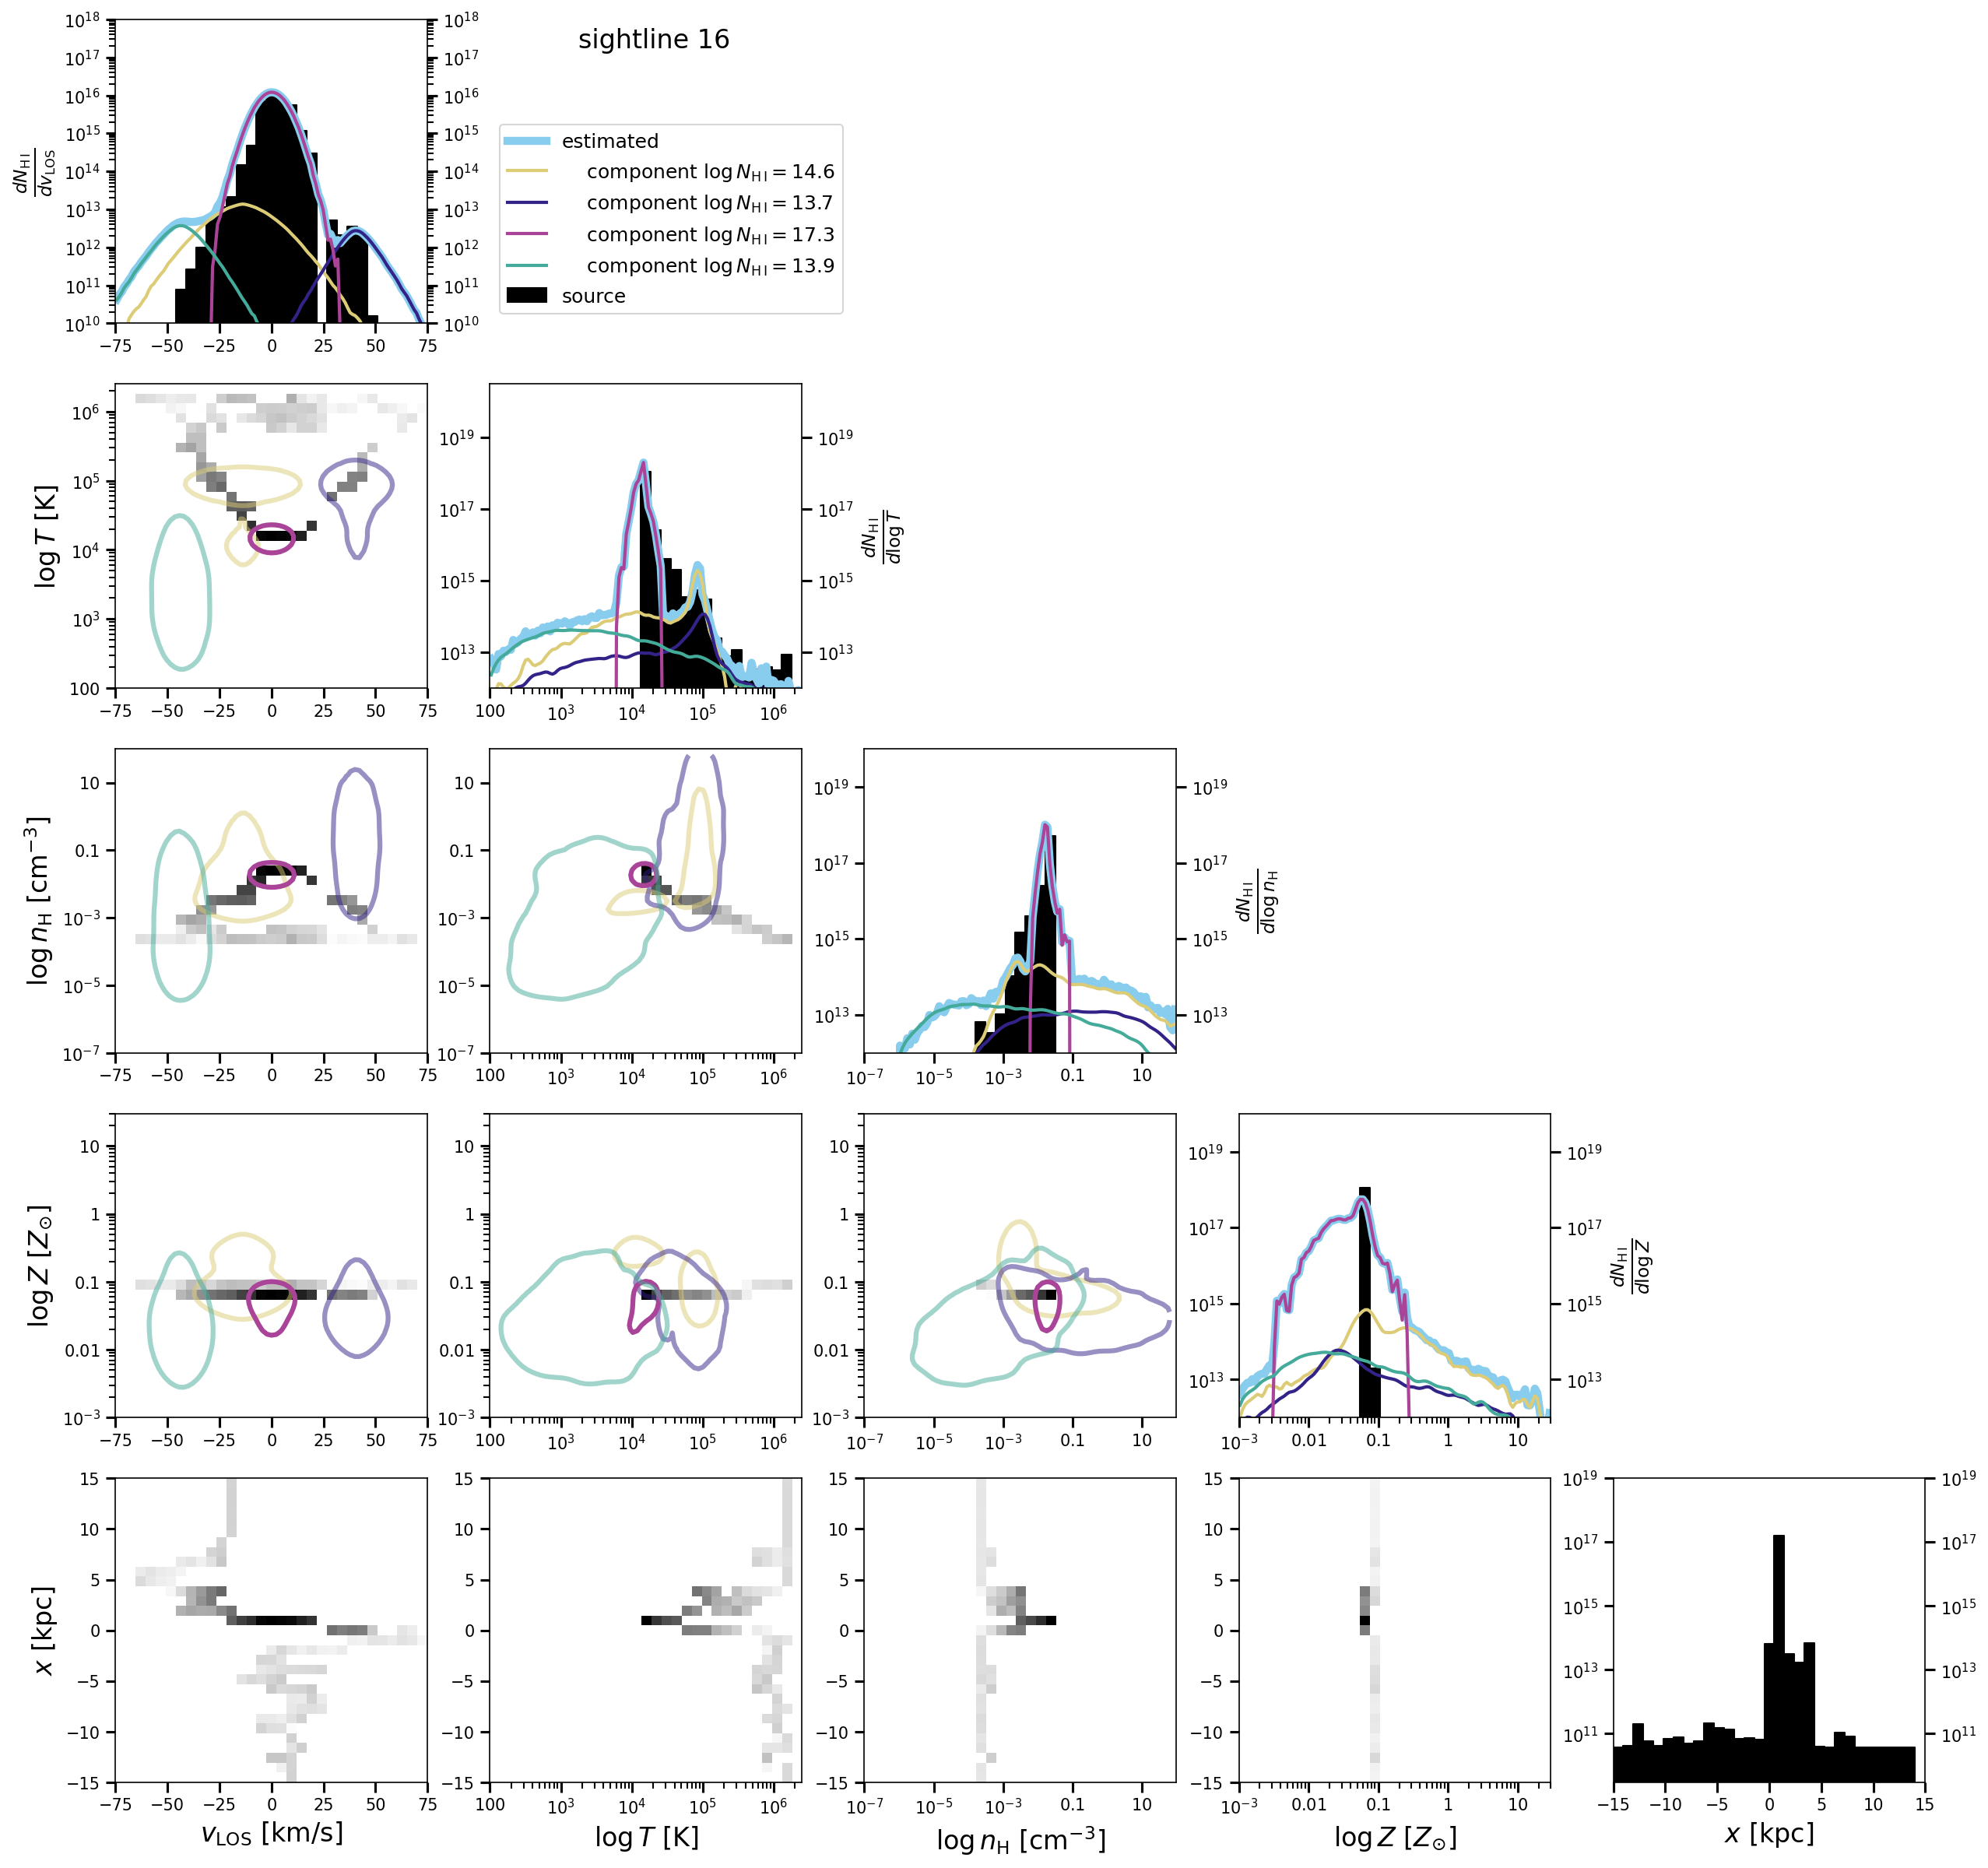
\includegraphics[height=0.45\textheight]{figures/sample2/high-z/sightline_0016.png}
    \label{f: sample2 16 corner}
    \caption{Same as Fig.~\ref{f: sample2 03}, but for sightline 16.}
\end{figure*}

\begin{figure*}
    \centering
    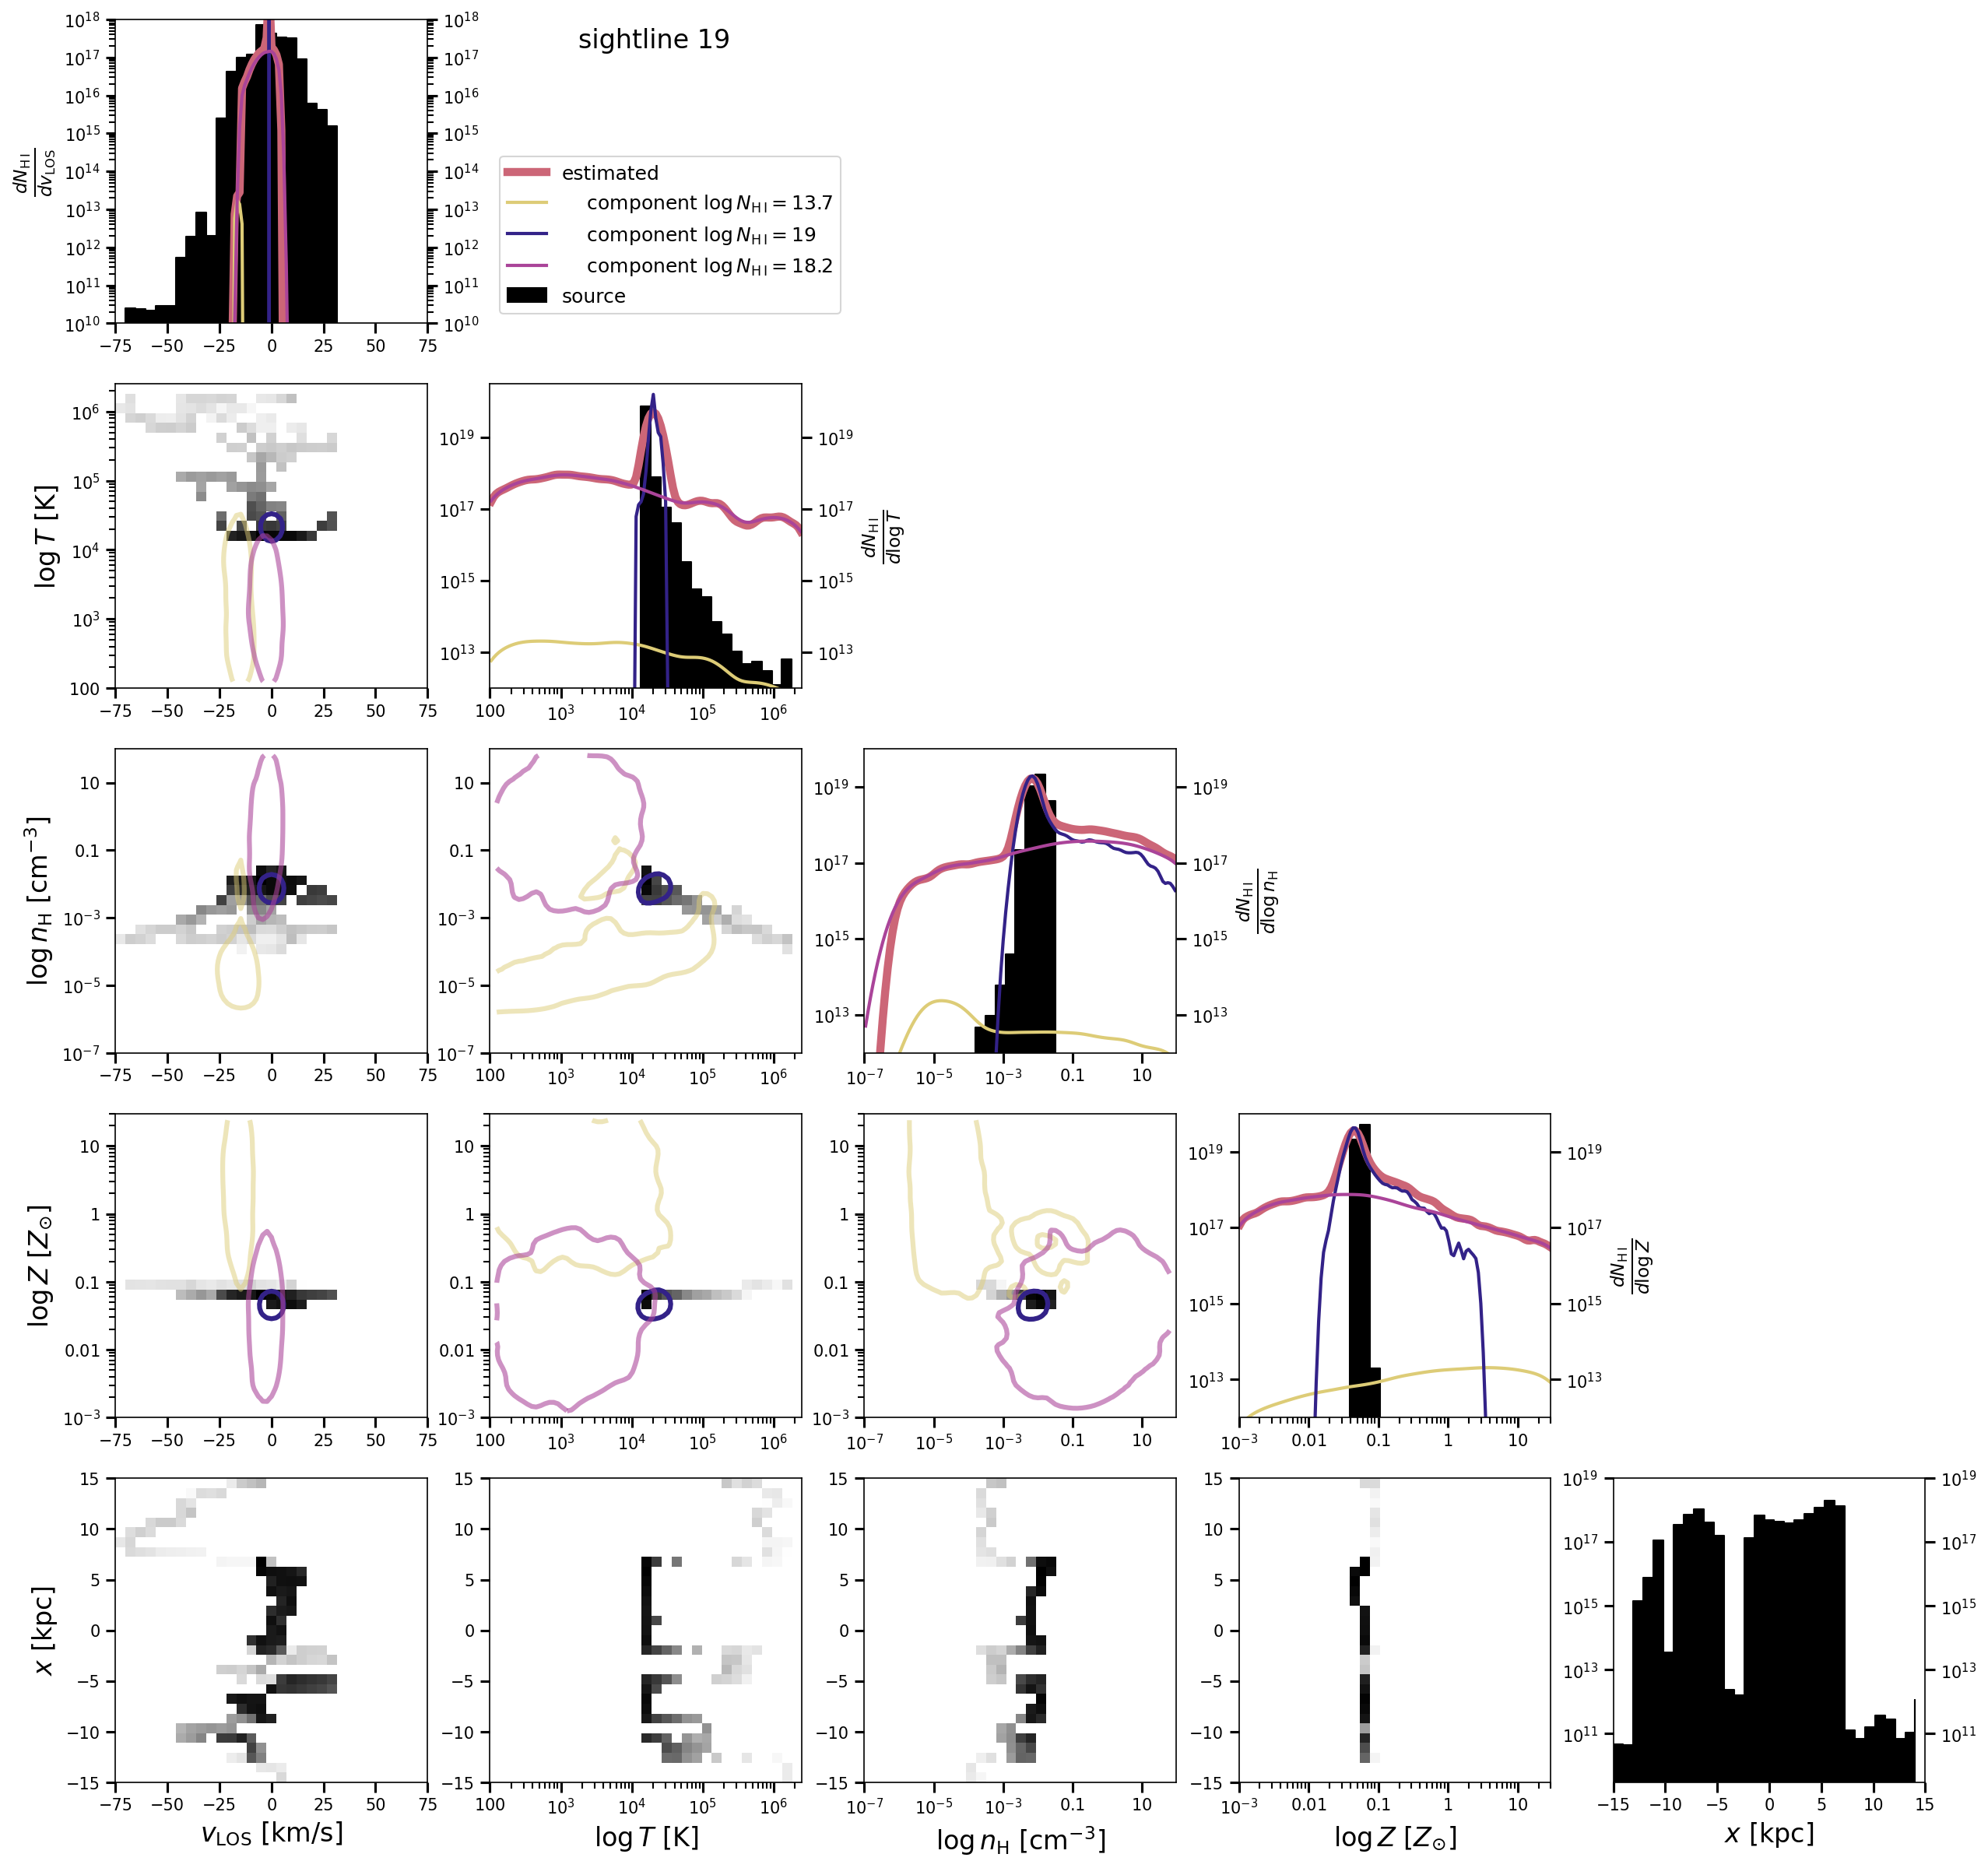
\includegraphics[height=0.45\textheight]{figures/sample2/original/sightline_0019.png}
    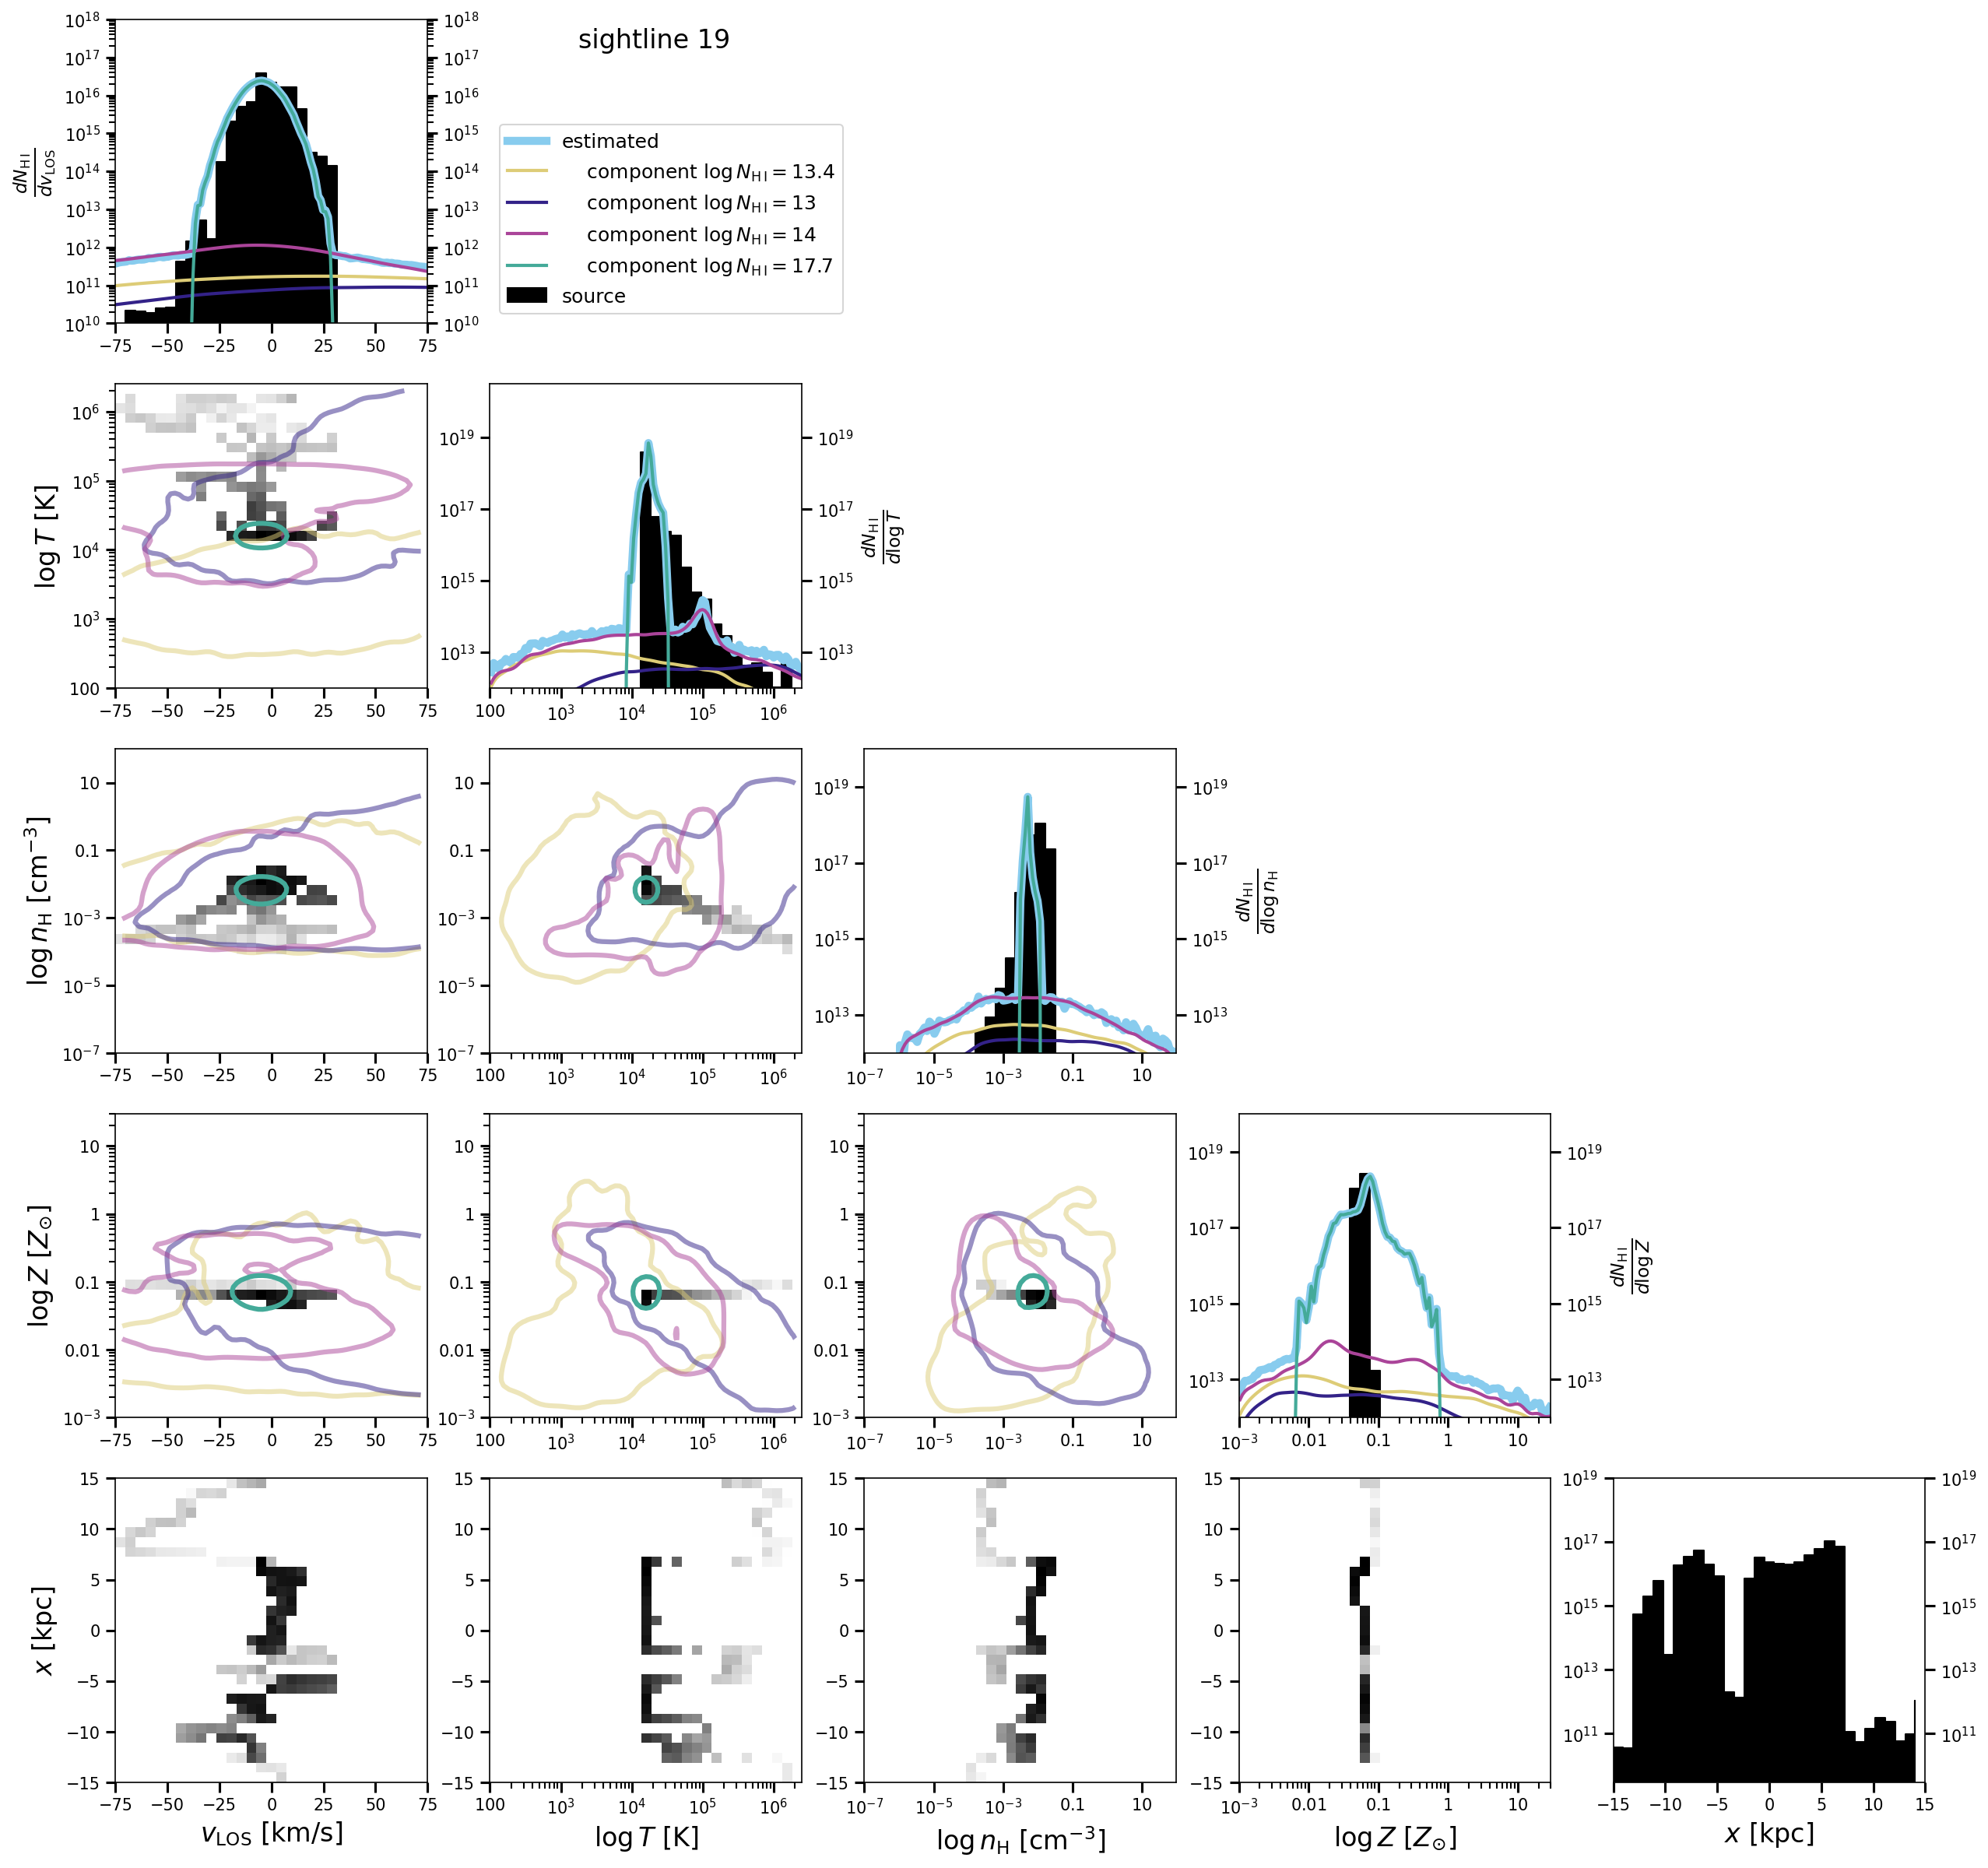
\includegraphics[height=0.45\textheight]{figures/sample2/high-z/sightline_0019.png}
    \label{f: sample2 19 corner}
    \caption{Same as Fig.~\ref{f: sample2 03}, but for sightline 19.}
\end{figure*}

This section includes additional figures for sample2.

%%%%%%%%%%%%%%%%%%%%%%%%%%%%%%%%%%%%%%%%%%%%%%%%%%


% Don't change these lines
\bsp	% typesetting comment
\label{lastpage}
\end{document}

% End of mnras_template.tex
